%\title{University of Bristol Thesis Template}
\RequirePackage[l2tabu]{nag}		% Warns for incorrect (obsolete) LaTeX usage
%
%
% File: memoirthesis.tex
% Author: Victor Brena
% Description: Contains the thesis template using memoir class,
% which is mainly based on book class but permits better control of 
% chapter styles for example. This template is an adaptation and 
% modification of Oscar's.
% 
% Memoir is a flexible class for typesetting poetry, fiction, 
% non-fiction and mathematical works as books, reports, articles or
% manuscripts. CTAN repository is found at:
% http://www.ctan.org/tex-archive/macros/latex/contrib/memoir/
%
%
% UoB guidelines for thesis presentation were found at:
% http://www.bris.ac.uk/esu/pg/pgrcop11-12topic.pdf#page=49
%
% UoB guidelines:
%
% The dissertation must be printed on A4 white paper. Paper up to A3 may be used
% for maps, plans, diagrams and illustrative material. Pages (apart from the
% preliminary pages) should normally be double-sided.
%
% Memoir class loads useful packages by default (see manual).
\documentclass[a4paper,11pt,leqno]{memoir} %add 'draft' to turn draft option on (see below)
%
%
% Adding metadata:
\usepackage{datetime}
\usepackage{ifpdf}
\ifpdf
\pdfinfo{
   /Author (Author's name)
   /Title (PhD Thesis)
   /Keywords (One; Two;Three)
   /CreationDate (D:\pdfdate)
}
\fi
% When draft option is on. 
\ifdraftdoc 
	\usepackage{draftwatermark}				%Sets watermarks up.
	\SetWatermarkScale{0.3}
	\SetWatermarkText{\bf Draft: \today}
\fi
%
% Declare figure/table as a subfloat.
\newsubfloat{figure}
\newsubfloat{table}
% Better page layout for A4 paper, see memoir manual.
\settrimmedsize{297mm}{210mm}{*}
\setlength{\trimtop}{0pt} 
\setlength{\trimedge}{\stockwidth} 
\addtolength{\trimedge}{-\paperwidth} 
\settypeblocksize{634pt}{448.13pt}{*} 
\setulmargins{4cm}{*}{*} 
\setlrmargins{*}{*}{1.5} 
\setmarginnotes{17pt}{51pt}{\onelineskip} 
\setheadfoot{\onelineskip}{2\onelineskip} 
\setheaderspaces{*}{2\onelineskip}{*} 
\checkandfixthelayout
%
\frenchspacing
% Font with math support: New Century Schoolbook
%
% UoB guidelines:
%
% Text should be in double or 1.5 line spacing, and font size should be
% chosen to ensure clarity and legibility for the main text and for any
% quotations and footnotes. Margins should allow for eventual hard binding.
%
% Note: This is automatically set by memoir class. Nevertheless \OnehalfSpacing 
% enables double spacing but leaves single spaced for captions for instance. 
\OnehalfSpacing 
%
% Sets numbering division level
\setsecnumdepth{subsection} 
%\maxsecnumdepth{subsubsection}
%
% Chapter style (taken and slightly modified from Lars Madsen Memoir Chapter 
% Styles document
\bibliographystyle{plain}
\usepackage{calc,soul,fourier}
\makeatletter 
\newlength\dlf@normtxtw 
\setlength\dlf@normtxtw{\textwidth} 
\newsavebox{\feline@chapter} 
\newcommand\feline@chapter@marker[1][4cm]{%
	\sbox\feline@chapter{% 
		\resizebox{!}{#1}{\fboxsep=1pt%
			\colorbox{gray}{\color{white}\thechapter}% 
		}}%
		\rotatebox{90}{% 
			\resizebox{%
				\heightof{\usebox{\feline@chapter}}+\depthof{\usebox{\feline@chapter}}}% 
			{!}{\scshape\so\@chapapp}}\quad%
		\raisebox{\depthof{\usebox{\feline@chapter}}}{\usebox{\feline@chapter}}%
} 
\newcommand\feline@chm[1][4cm]{%
	\sbox\feline@chapter{\feline@chapter@marker[#1]}% 
	\makebox[0pt][c]{% aka \rlap
		\makebox[1cm][r]{\usebox\feline@chapter}%
	}}
\makechapterstyle{daleifmodif}{
	\renewcommand\chapnamefont{\normalfont\Large\scshape\raggedleft\so} 
	\renewcommand\chaptitlefont{\normalfont\Large\bfseries\scshape} 
	\renewcommand\chapternamenum{} \renewcommand\printchaptername{} 
	\renewcommand\printchapternum{\null\hfill\feline@chm[2.5cm]\par} 
	\renewcommand\afterchapternum{\par\vskip\midchapskip} 
	\renewcommand\printchaptertitle[1]{\color{gray}\chaptitlefont\raggedleft ##1\par}
} 
\makeatother 
\chapterstyle{daleifmodif}
%
% UoB guidelines:
%
% The pages should be numbered consecutively at the bottom centre of the
% page.
\makepagestyle{myvf} 
\makeoddfoot{myvf}{}{\thepage}{} 
\makeevenfoot{myvf}{}{\thepage}{} 
\makeheadrule{myvf}{\textwidth}{\normalrulethickness} 
\makeevenhead{myvf}{\small\textsc{\leftmark}}{}{} 
\makeoddhead{myvf}{}{}{\small\textsc{\rightmark}}
\pagestyle{myvf}
%
% Oscar's command (it works):
% Fills blank pages until next odd-numbered page. Used to emulate single-sided
% frontmatter. This will work for title, abstract and declaration. Though the
% contents sections will each start on an odd-numbered page they will
% spill over onto the even-numbered pages if extending beyond one page
% (hopefully, this is ok).
\newcommand{\clearemptydoublepage}{\newpage{\thispagestyle{empty}\cleardoublepage}}
%
%
% Creates indexes for Table of Contents, List of Figures, List of Tables and Index
\makeindex
% \printglossaries below creates a list of abbreviations. \gls and related
% commands are then used throughout the text, so that latex can automatically
% keep track of which abbreviations have already been defined in the text.
%
% The import command enables each chapter tex file to use relative paths when
% accessing supplementary files. For example, to include
% chapters/brewing/images/figure1.png from chapters/brewing/brewing.tex we can
% use
% \includegraphics{images/figure1}
% instead of
% \includegraphics{chapters/brewing/images/figure1}
\usepackage{import}

% Add other packages needed for chapters here. For example:
\usepackage{lipsum}					%Needed to create dummy text
\usepackage{newlfont}					%Helpful package for fonts and symbols
\usepackage{layouts}					%Layout diagrams
\usepackage{graphicx}					%Calls figure environment
\usepackage{longtable,rotating}			%Long tab environments including rotation. 	%Needed to encode non-english characters 
									%directly for mac
\usepackage{colortbl}					%Makes coloured tables			%Even more math symbols
\usepackage{float}						%Helps to place figures, tables, etc. 
\usepackage{verbatim}					%Permits pre-formated text insertion
\usepackage{upgreek }					%Calls other kind of greek alphabet
\usepackage{latexsym}					%Extra symbols
\usepackage[square,numbers,
		     sort&compress]{natbib}		%Calls bibliography commands 
\usepackage{url}						%Supports url commands
\usepackage{etex}						%eTeXÕs extended support for counters
\usepackage{fixltx2e}					%Eliminates some in felicities of the 
									%original LaTeX kernel	%For languages characters and hyphenation
\usepackage{color}                    				%Creates coloured text and background
\usepackage[colorlinks=true,
		     allcolors=black]{hyperref}              %Creates hyperlinks in cross references
\usepackage{memhfixc}					%Must be used on memoir document 
									%class after hyperref
\usepackage{enumerate}					%For enumeration counter
\usepackage{footnote}					%For footnotes
\usepackage{microtype}					%Makes pdf look better.
\usepackage{rotfloat}					%For rotating and float environments as tables, 
									%figures, etc. 
\usepackage{alltt}						%LaTeX commands are not disabled in 
									%verbatim-like environment
\usepackage[version=0.96]{pgf}			%PGF/TikZ is a tandem of languages for producing vector graphics from a 
\usepackage{tikz}						%geometric/algebraic description.
\usetikzlibrary{arrows,shapes,snakes,
		       automata,backgrounds,
		       petri,topaths}				%To use diverse features from tikz		
%							
%Reduce widows  (the last line of a paragraph at the start of a page) and orphans 
% (the first line of paragraph at the end of a page)
\widowpenalty=1000
\clubpenalty=1000
%
% New command definitions for my thesis
%
\newcommand{\keywords}[1]{\par\noindent{\small{\bf Keywords:} #1}} %Defines keywords small section
\newcommand{\parcial}[2]{\frac{\partial#1}{\partial#2}}                             %Defines a partial operator
\newcommand{\vectorr}[1]{\mathbf{#1}}                                                        %Defines a bold vector
\newcommand{\vecol}[2]{\left(                                                                         %Defines a column vector
	\begin{array}{c} 
		\displaystyle#1 \\
		\displaystyle#2
	\end{array}\right)}
\newcommand{\mados}[4]{\left(                                                                       %Defines a 2x2 matrix
	\begin{array}{cc}
		\displaystyle#1 &\displaystyle #2 \\
		\displaystyle#3 & \displaystyle#4
	\end{array}\right)}
\newcommand{\pgftextcircled}[1]{                                                                    %Defines encircled text
    \setbox0=\hbox{#1}%
    \dimen0\wd0%
    \divide\dimen0 by 2%
    \begin{tikzpicture}[baseline=(a.base)]%
        \useasboundingbox (-\the\dimen0,0pt) rectangle (\the\dimen0,1pt);
        \node[circle,draw,outer sep=0pt,inner sep=0.1ex] (a) {#1};
    \end{tikzpicture}
}
\newcommand{\range}[1]{\textnormal{range }#1}                                             %Defines range operator
\newcommand{\innerp}[2]{\left\langle#1,#2\right\rangle}                                 %Defines inner product
\newcommand{\prom}[1]{\left\langle#1\right\rangle}                                         %Defines average operator
\newcommand{\tra}[1]{\textnormal{tra} \: #1}                                                       %Defines trace operator
\newcommand{\sign}[1]{\textnormal{sign\,}#1}                                                   %Defines sign operator
\newcommand{\sech}[1]{\textnormal{sech} #1}                                                  %Defines sech
\newcommand{\diag}[1]{\textnormal{diag} #1}                                                    %Defines diag operator
\newcommand{\arcsech}[1]{\textnormal{arcsech} #1}                                       %Defines arcsech
\newcommand{\arctanh}[1]{\textnormal{arctanh} #1}                                         %Defines arctanh
%Change tombstone symbol
\newcommand{\blackged}{\hfill$\blacksquare$}
\newcommand{\whiteged}{\hfill$\square$}

%
%
% New definition of square root:
% it renames \sqrt as \oldsqrt
\let\oldsqrt\sqrt
% it defines the new \sqrt in terms of the old one
\def\sqrt{\mathpalette\DHLhksqrt}
\def\DHLhksqrt#1#2{%
\setbox0=\hbox{$#1\oldsqrt{#2\,}$}\dimen0=\ht0
\advance\dimen0-0.2\ht0
\setbox2=\hbox{\vrule height\ht0 depth -\dimen0}%
{\box0\lower0.4pt\box2}}
%
% My caption style
\newcommand{\mycaption}[2][\@empty]{
	\captionnamefont{\scshape} 
	\changecaptionwidth
	\captionwidth{0.9\linewidth}
	\captiondelim{.\:} 
	\indentcaption{0.75cm}
	\captionstyle[\centering]{}
	\setlength{\belowcaptionskip}{10pt}
	\ifx \@empty#1 \caption{#2}\else \caption[#1]{#2}
}
%
% My subcaption style
\newcommand{\mysubcaption}[2][\@empty]{
	\subcaptionsize{\small}
	\hangsubcaption
	\subcaptionlabelfont{\rmfamily}
	\sidecapstyle{\raggedright}
	\setlength{\belowcaptionskip}{10pt}
	\ifx \@empty#1 \subcaption{#2}\else \subcaption[#1]{#2}
}
%
%An initial of the very first character of the content
\usepackage{lettrine}
\newcommand{\initial}[1]{%
	\lettrine[lines=3,lhang=0.33,nindent=0em]{
		\color{gray}
     		{\textsc{#1}}}{}}
%
%
% Hyphenation for some words
%
\hyphenation{res-pec-tively}
\hyphenation{mono-ti-ca-lly}
\hyphenation{hypo-the-sis}
\hyphenation{para-me-ters}
\hyphenation{sol-va-bi-li-ty}
%
%
\graphicspath{{images/}}
\linespread{1}
\usepackage{wrapfig}
\usepackage{amsfonts}
\usepackage{amsmath}
\usepackage[utf8]{inputenc}
\usepackage[T1]{fontenc}
\usepackage{graphicx}
\usepackage[english]{babel}
\usepackage[algoruled]{algorithm2e}

\renewcommand{\theequation}{\thesection.arabic{equation}}

\renewcommand{\thefigure}{\thesection.\arabic{figure}}



\renewcommand{\vec}[1]{\mathbf{#1}}
\renewcommand{\theequation}{\thesubsection.\arabic{equation}}
\DeclareGraphicsExtensions{.pdf,.png,.jpg, .gif}

\usepackage{amsthm}

\usepackage[english]{babel}
\usepackage{mathtools}

%\usepackage[OT2,T1]{fontenc}
%\DeclareSymbolFont{cyrletters}{OT2}{wncyr}{m}{n}
%\DeclareMathSymbol{\sha}{\mathalpha}{cyrletters}{"58}

\DeclareFontFamily{U}{wncy}{}
\DeclareFontShape{U}{wncy}{m}{n}{<->wncyr10}{}
\DeclareSymbolFont{mcy}{U}{wncy}{m}{n}
\DeclareMathSymbol{\Sh}{\mathord}{mcy}{"58} 
\DeclareMathOperator*{\argmin}{arg\,min}

\newcounter{eqn}
\renewcommand*{\theeqn}{\alph{eqn})}
\newcommand{\num}{\refstepcounter{eqn}\text{\theeqn}\;}

\makeatother
\newcommand{\vectornorm}[1]{\left|\left|#1\right|\right|}
\newcommand*\conjugate[1]{\bar{#1}}


\newtheorem{thm}{Theorem}
\newtheorem{defn}{Definition}
 %\theoremstyle{plain}
  \newtheorem{theorem}{Theorem}[section]
  \newtheorem{corollary}[theorem]{Corollary}
  \newtheorem{proposition}[theorem]{Proposition}
  \newtheorem{lemma}[theorem]{Lemma}
\newtheorem{example}[theorem]{Example}
  \newtheorem{definition}[theorem]{Definition}
  \newtheorem{conj}[theorem]{Conjecture}
 \newtheorem{condition}{Condition}
 \newtheorem{remark}[theorem]{Remark}

\newcommand{\supp}{\operatorname{supp}} 
\newcommand{\vc}[1]{{\mathbf{ #1}}}
\newcommand{\tn}{\widetilde{\nabla}_{n} }
\newcommand{\Z}{{\mathbb{Z}}}
\newcommand{\re}{{\mathbb{R}}}
\newcommand{\II}{{\mathbb{I}}}
\newcommand{\ep}{{\mathbb{E}}}
\newcommand{\pr}{{\mathbb{P}}}
\newcommand{\FF}{{\mathcal{F}}}
\newcommand{\TT}{{\mathcal{T}}}
\newcommand{\phin}{\phig{n}}
\newcommand{\phig}[1]{\phi^{(#1)}}
\newcommand{\ol}[1]{\overline{#1}}
\newcommand{\eff}{{\rm eff}}
\newcommand{\suc}{{\rm suc}}
\newcommand{\tends}{\rightarrow \infty}
\newcommand{\setS}{{\mathcal{S}}}
\newcommand{\setP}{{\mathcal{P}}}
\newcommand{\setX}{{\mathcal{X}}}
\newcommand{\nec}{{\rm nec}}
\newcommand{\bd}{{\rm bd}}
\usepackage{glossaries}
\newacronym{cmux}{CMUX}{Compressive Multiplexer}
\newacronym{rd}{RD}{Random Demodulator}
\newacronym{mwc}{MWC}{Modulated Wideband Converter}
\newacronym{pu}{PU}{Primary User}
\newacronym{fc}{FC}{Fusion Centre}
\newacronym{cr}{CR}{Cognitie Radio}
\newacronym{mmv}{MMV}{Multiple Measurement Vector}
\newacronym{cs}{CS}{Compressive Sensing}
\numberwithin{equation}{chapter}
\begin{document}

% UoB guidlines:
%
% Preliminary pages
% 
% The five preliminary pages must be the Title Page, Abstract, Dedication
% and Acknowledgements, Author's Declaration and Table of Contents.
% These should be single-sided.
% 
% Table of contents, list of tables and illustrative material
% 
% The table of contents must list, with page numbers, all chapters,
 % sections and subsections, the list of references, bibliography, list of
% abbreviations and appendices. The list of tables and illustrations
% should follow the table of contents, listing with page numbers the
% tables, photographs, diagrams, etc., in the order in which they appear
% in the text.
% 
\frontmatter
\pagenumbering{roman}
%
%\input{frontmatter/title}
%\clearemptydoublepage
%
%\input{frontmatter/abstract}
%\clearemptydoublepage
%
%\input{frontmatter/dedication}
%\clearemptydoublepage
%
%\input{frontmatter/declaration}
%\clearemptydoublepage
%
\renewcommand{\contentsname}{Table of Contents}
\maxtocdepth{subsection}
\tableofcontents*
\addtocontents{toc}{\par\nobreak \mbox{}\hfill{\bf Page}\par\nobreak}
\clearemptydoublepage
%
%\listoftables
%\addtocontents{lot}{\par\nobreak\textbf{{\scshape Table} \hfill Page}\par\nobreak}
%\clearemptydoublepage
%
\listoffigures
\addtocontents{lof}{\par\nobreak\textbf{{\scshape Figure} \hfill Page}\par\nobreak}
\clearemptydoublepage
%
%
% The bulk of the document is delegated to these chapter files in
% subdirectories.
\mainmatter
%
%\import{chapters/chapter01/}{chap01.tex}
%\clearemptydoublepage
%

\chapter{Introduction}
\section{Introduction}

In order to meet exponentially growing consumer demand for wireless data, radio spectrum regulators considering opportunistic spectrum access policies. Historic spectrum regulation focussed on exclusive frequency assignments (licensing), with spatial and frequency separation to mitigate interference between users. However, this approach leads to considerable underutilisation in both space and time. Thus, faced with a need to provide 1000 times the bandwidth in 10 years, regulators are considering agile access technologies on a licence exempt basis.

Before opportunistic access is a reality, speedy, robust, and accurate estimation of frequency spectra must be made. This is a challenging statistical and engineering problem, limited by characteristics of wireless channels such as multipath fading, and shadowing. The proposed bands have a large bandwidth, containing sub-channels which are not contiguous but statistically correlated, and radio-wave fading environment which can mask high-powered transmissions. Traditional methods are un-viable in these conditions; either requiring expensive hardware to meet the data rate required to perform the sampling, or a large number of RF components to turn a single wideband channel into many narrowband ones.

This project addresses the issue of estimating available frequencies for opportunistic transmission, from a set of underdetermined measurements. The compete set of measurements may be available to a particular sensor. Or, the measurements may be distributed over a network of sensors, improving estimation accuracy, and 

The growing number of wireless devices is placing increasing demand on radio spectrum. Consumers are demanding faster speeds and better quality connections in more places. However, there is a limited amount of frequencies to transmit on. Consequently, demand for frequencies which provide sufficient bandwidth, good range and in-building penetration is high.

Not all frequencies are used at all times and in all places. Judicious spectrum management could alleviate the issue of too few frequencies being available to devices by developing approaches to interleaving opportunistic transmissions within established bands. 

There are benefits to spectrum sharing beyond simply satisfying consumer demand. Innovative wireless applications such as wireless rural broadband, remote monitoring, and machine-to-machine applications will be made viable without the need to purchase exclusive access to a specific frequency. 

The historic allocation process has placed unused spectrum between adjacent radio channels, in an attempt to avoid interference between consecutive users. However, technical changes in transmission standards are making some bands available as modern coding and modulation techniques are more spectrally efficient. In particular, in the UK, the switchover from analogue to digital terrestrial broadcast has freed many previously used bands.

Recent regulatory focus has been on frequencies in the TV broadcast bands 470-790MHz. In the UK, TV channels are broadcast using up to six multiplexes, each requiring an 8MHz channel. A total of 32 of these channels are allocated for TV broadcast, whilst only 6 of these channels are required to receive the 6 multiplexes at any given location. This is because TV broadcast is high powered and needs spatial separation between coverage areas to avoid interference. As such, the majority of TV frequencies reserved for TV broadcast are unused in any given place. These white spaces are spectrum which has been left over to prevent interference between primary users (such as TV broadcast). These frequencies can be used on an opportunistic basis by relatively low-powered devices. Whilst current focus is on the TVWS bands, the work presented in this thesis can be used in other, as yet unrealised frequencies.

Currently access to spectrum is managed in two ways: licensed and license exempt access. Licensing authorises a particular user/users to exclusive use of a specific frequency band. License exempt access allows any user to access a band, provided they meet technical requirements intended to limit interference in on other users. This is a particularly pressing issue for the co-existence of licensed users and licence exempt users in the same band.

Devices seeking to access white spaces need a robust mechanism for learning which frequencies can be used at a particular time and location. The approach currently being taken by OFCOM and the FCC is to maintain a set of databases, which map the location of white spaces based on knowledge of existing spectrum users. An alternative approach is for devices to monitor the use of spectrum individually.

One approach to white-space access is to maintain a database of currently available frequencies. The database would contain up to date information about incumbents, including television transmitters and wireless microphones. It would also need to maintain information about currently operative secondary users. Devices would register with the database, based on their geo-location and the service would determine availability for the device, either based on in situ measurements, or from a propagation model.

Location based measurements are a costly approach, as they need to be redone every time primary user transmission characteristics change, and they cannot be done economically in difficult to reach places. Propagation models can achieve good accuracy, but at the cost of being complex and computationally intensive. Simplistic models do not agree with ground truth measurements. 

Devices must also supply geographic information to a database service. How this is done has yet to be codified, but current methodologies all have drawbacks. GPS positioning works well outdoors, but is inaccurate indoors. Cellular location can yield errors of up to a mile. Using the base-station location as a proxy for the device location results in an unacceptably high loss of whitespaces, as decisions would have to be needlessly conservative.

An alternative to maintaining a database of available frequencies, is for secondary users to independently sense spectrum. This method is subject to a number of technical limitations. The proposed bands have an ultra-wide bandwidth. Traditional sensing approaches to this have been either to divide the band into a number of contiguous narrow bands, or to simply use a high rate processing device to capture the necessary samples. Both methods are prohibitively expensive, and require dedicated and energy hungry hardware. Further, traditional statistical spectral detection and estimation techniques make assumptions about the primary users signal. Such assumptions include cyclo-stationarity, the presence of specific waveform patters, the use of known pilot sequences, and sufficiently high powered transmissions that energy detection is viable. In practice, some (or all) of these assumptions are violated; either because assumed patterns are not present in the  transmission, or because the radio environment has a deep fade between the primary and secondary user masking high powered transmissions.

The biggest issues for single node sensing are multipath fading, shadowing, and PU receiver uncertainty. Cooperation between a network of nodes can improve sensing performance through spatial diversity. In cooperative sensing information from geographically diverse nodes is aggregated in the decision making process. Combining observations can overcome the deficiencies of observations unique to individual cognitive radios. Spatial diversity makes it unlikely that all radios will experience the same fading and receiver uncertainty. Approaches to cooperative sensing based on Nyquist sensing typically involve energy detection at each node, along with a gain combining procedure (which is either performed at a fusion node, or via a decentralised algorithm). Cooperative sensing can use such simple methods at each node as receiver sensitivity can be mitigated by using multiple statistically independent observations. This reduces the complexity and cost of the individual cognitive radios.

Cooperative sensing has drawbacks however. Spatial diversity does not necessarily mean statistically independent observations. A subset of nodes all blocked by the same object will make measurements which are correlated and corrupted by the same shadowing for example. Cooperative sensing also involves an overhead with the being part of a network. This is any extra time, energy and processing when compared to sensing individually. 

An alternative sensing strategy is compressive sampling (CS). This is a new paradigm in signal processing which has emerged over the last decade, and has had significant success in imaging problems. In particular compressive sampling strategies have reduced the time needed for an MRI scan from 2 minutes to 30 seconds. Patients previously had to hold their breath for the entire duration. The central innovation in compressive sensing is that randomness is an effective strategy for sensing sparse signals. In practice much of the TVWS spectrum is unoccupied, and CS can leverage this sparsity to reduced the sampling rate of the CRS.

Group Testing is a model sparse inference problem, first introduced by Dorfmann in the context of testing for rare disease. Given a population of items, some small fraction of which has an interesting property (labelled defective), Group Testing proposes algorithms to find those items efficiently. What allows these items to be discovered, in fewer tests than the total number of items, is testing pools of items. That is, items aren't tested individually, but several together. In testing for rare diseases the blood samples are mixed and the mixture is tested. This allows fast elimination of non-defective items. Popular pooling designs are randomised - items are included in a test with independent probabilities. We consider probabilistic algorithms with non uniform probabilities of each item's defectivity. These non-uniform priors could come from a TVWS database of possibly occupied spectrum, or from summarising risk and family history in disease testing.

In this thesis, we argue that in order to perform spectrum sensing n the TVWS band, at reasonable sampling rates we must exploit the new sensing paridigm of compressive sensing. We show how we can quantify the reduction in absolute number of samples needed to accuractely reconstruct a signal using this methodology. We diwcuss how the sample rate at a single node may still be too high even with the reduced rate, and we provide two approaches to reducing it even further. We also  discuss how with use the TVWS band may no longer be sparse, in the frequency basis. To recify this, we propose a distributed model of the spectral gradient, which allows us to accurately reconstruct the frequency bamd. We do this via an improved version of distributed ADMM. To reduce the smapling rate at a single device, we propose to aviod reconstruction altogether. We show it is possible to determine whether a frequency range is occupied with as little as 5% of the samples required by Nyquist sampling.  

The structure of this thesis is as follows. Chapter 2 covers the relevant material on Nyquist sensing theory and Nyquist approaches to the spectrum sensing problem. Nyqusit sensing is introuduced, and how to reconstruct the signal from its samples is covered. Then, what the spectrum sensing problem is is defined, along with narrowband approaches such as energy detection, feature detection, and matched filtering - in order of increasing complexity. Distributed and cooperative approaches to the problem are then dicussed, in particular the AND and OR rules of equal gain combining. We discuss that distrbuted approaches have better statistical performance due to spatial diversity, but that each sensor still needs to use the same number of samples as the single sensor problem. It is argued that the data rates demanded by TVWS sensing makes this Nyquist approach unfeasible, and that some mechanism of reducing the absolute number samples is required for spectrum sensing in the TVWS band to be a reality. 

Chapter 3 covers the theory of compressive sensing and some previous applications to the Wideband Spectrum sensing. In particular, the conditions under which a sparse high-dimensional vector can be recovered from undersampled representations are introduced - the Restriced Isometry Property (RIP) and stable embeddings along with which sensing operators satisfy these conditions. Then three families of reconstruction algorithm are discussed: greedy, convex and Bayesian. The relative merits and demerits of these alogorithms are compared in terms of speed, accuracy, complexity, and undersampling performance are discussed, concluding that more accurate algorithms which can reconstruct from fewer samples are slower and more complex. Two compressive approches to Wideband Spectrum sensing are then discussed in depth: the Random Demodulator and the Modulated Wideband Coverter, before moving on to discuss distributed compressive sensing.  

Chapter 4 covers the theory of ADMM. It starts with the a potted history of the algorithm - from solving the heat equation to optimisation in Hilbert spaces - and some applictaions, including imaging and predictive control problems. Then the theory of the Proximity operator is covered, and its connection to ADMM, along with examples pertinent to high-dimensional statistical signal processing. The introduction of the Prox operator is motivated by how it allows simple calculation of the sub-problems in ADMM. Thus, difficult non-smooth optimisation can be quickly performed in simpler stages.

Chapter 5 is new material and covers the application of and optimisation on graphs.

Chapter 6 introduces a model of 

Chapter 7 covers compressive inference

Chapter 8 covers the application of our methods to real world data sets.

Finally, Chapter 9 covers group testing and our approach to .

Despite the ubiquity, capacity and apparent efficacy, modern communication systems are wasteful, inefficient and in need of reform. Most of the bits of data collected by our sensing systems are unessential, and only serve to necessitate data compression wasting computation time before transmission. For example, people regularly use a camera with a resolution of several megapixels only to upload a file of a few kilobytes to Facebook. Devices are unable to make dynamic decisions about how to transmit this data, leading to both spectral exhaustion on some frequencies whilst much of the available radio spectrum lies fallow. 

This project addresses these issues, by reviewing a novel acquisition and decompression framework for data: a way in which we need only sense the most informative bits of data. This framework is then applied to the problem of sensing spectral opportunities dynamically, to make better use of available spectrum. 

The key uniting both these applications is that data and spectra are \textit{sparse}: that is they have a representations which are 'smaller' than their respective dimension. For example, images and audio can be compressed into file formats much smaller than when initially recorded (compare the relative sizes of bitmap and JPEG images).

The sole focus of this research is to use the sparsity of the spectrum to uncover transmission opportunities, allowing better use of spectrum more generally. 

We are motivated by the need to send more data over wireless networks, whilst at the same time having a constrained frequency set over which to transmit this information. This issue could be alleviated by users dynamically allocating spectrum on a per-transmission basis: without the ability to gain knowledge of spectral conditions this can never become a reality however. 

The requirement for increasing bandwidth isn't just a pressing issue for today: in the next decade it is forecast that network operators will need to provide for three-orders of magnitude (1000 times) more capacity. Demand is continually outstripping supply - motivated by the ubiquity of smart-phones, and the consumers appetites for media. 

At the same time as this demand for ever more data, there is an increasing scarcity of radio spectrum over which to transmit. New frequencies are rarely cleared for commercial purposes, and when they are they go for high prices.  A decade ago the UK auction for 3G spectrum licenses raised an estimated 22.4 billion pounds for the UK treasury, indicating the seriousness of the market players requirements for new spectrum. The recent 4G spectrum auction raised 2.3 billion pounds with initial networks being rolled out by the end of 2013.

\begin{figure*}[h]
\centering
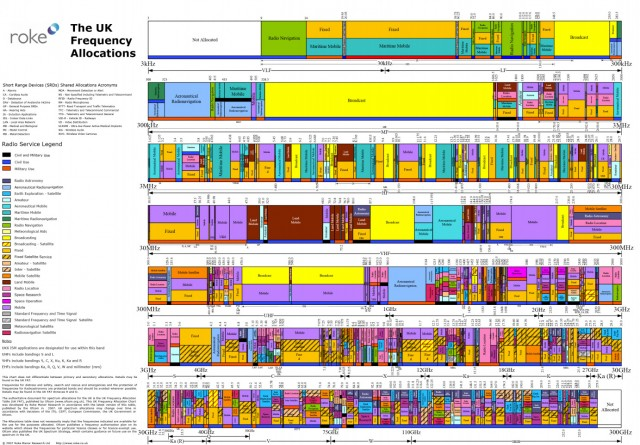
\includegraphics[height = 7 cm]{uk-spectrum-allocation-chart1-640x445.jpg}
\caption{A digram of current Spectral allocation \cite{Strategy2013}}
\label{spectrumalloc}
\end{figure*}

However, a closer inspection of the frequency allocation suggests this scarcity is artificial, it's more a product of regulatory oversight over time. As the constraints on spectrum requirement became more complex, so did the solutions to that problem - at the cost of leaving much of the spectrum idle for most of the time. 

For example: much of the spectrum is allocated to TV broadcast, radio broadcast and mobile. However, if we look closer, the allocations aren't even for specific companies - they're simply categories. Within these, OFCOM may have many licensees within each category.

Also interesting to note is how much frequency the Government allocates to itself (the red bar underneath the blocks indicates Government use). Compare this to the actual utilisation of spectrum: much of it is not used at all. Figure \ref{frequtil} shows a snapshot of frequency utilisation in three diverse locations in the UK over te radio specturm, note that many frequencies are not utilised (coloured blue) whilst others have significant activity (coloured yellow). Note that the plot for Southwark (central London) is barely different from Braddock - a rural area. 

\begin{figure*}[h]
\centering
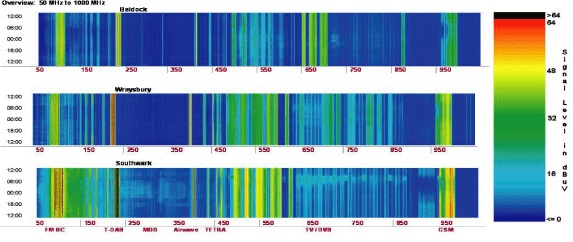
\includegraphics[height = 7 cm, width=0.5\textwidth]{cr2.jpg}
\caption{A snapshot of frequency utilisation in various areas: many frequencies are not used at all, whilst there is significant activity on others \cite{Burbidge2007}}
\label{frequtil}
\end{figure*}

How do we then go about solving this issue - how can we obtain the most significant bits of information from our sensing mechanism, whilst obviating the need to compress the data once we are done? How do we dynamically assign spectrum? The work of Candes, Tao \cite{Candes2006} and Donoho \cite{donoho2}, has shown that instead of measuring the information we require directly (and then compressing it), we can measure 'holographic' and non-linear random projections between our measurement space and the space where our data is sparse. This requires only the knowledge that the signal is compressible via some transform - both the acquisition protocol and the reconstruction algorithm are agnostic to the type of signal. What is surprising is that the sampling kernels are fixed independently of the signal, are non-adaptive and these projections are sufficient to reconstruct the signal - as if we had an Oracle to tell us where the non-zero components of our signal are. 

This work has had a large impact in medical imaging since it's inception: for example, it's now possible to take an image of a patient's heart within a single breath, as well as dynamic imaging of the heart (\cite{Donoho} figures 7 and 9).

Modern digital signal processing techniques (such as modulation techniques) are far more spectrally efficient than their historic analogue counterparts, which has in part contributed to the spectrum crisis. All this is changing though: from the beginning of 2013 all TV in the UK will transmitted digitally. Historically, television in the UK was broadcast using analogue signals requiring 32 multiplexes. Digital TV requires 6 multiplexes, on the other hand. 

This freeing up of TV frequencies represents an opportunity: these frequencies have good propagation characteristics (they suffer less with free space path loss relative to higher frequencies), whilst sill providing good bandwidth for data transmission. These TV frequencies are being opened up to civilian and  commercial users: spectral holes will be able to be exploited opportunistically by devices, so long as they don't interfere with the reception of TV. Historically, this is the single largest gift of new spectrum, and because there is no requirement for licensing this spectrum is free.

As with all technological innovations, this will not only improve existing infrastructure but also new classes of devices to transmit, for instance; applications such as passive sensor networks) which only need spectrum intermittently to transmit monitoring results), inter-vehicle communication for real time traffic monitoring and wireless internet at broadband data rates have all been proposed.

Despite all of this hype, dynamic spectrum access won't become a reality unless spectral holes can be robustly detected. The requirement that secondary users exploit the new spectrum politely, without interference to primary user makes spectrum sensing essential to TV white-space (TVWS) technologies. The realisation of any Cognitive Radio standard (such as IEEE 802.22), requires the co-existence of primary (TV users) and secondary (everybody else who wants to use TVWS spectrum) users of the frequency spectrum to ensure proper interference mitigation and appropriate network behaviour. 

Users of TVWS (Cognitive Radios) must sense whether spectrum is available, and must be able to detect very weak primary user signals. Furthermore they must sense over a wide bandwidth (due to the amount of TVWS spectrum proposed), which challenges traditional Nyquist sampling techniques, because the sampling rates required are not technically feasible with current RF or Analogue-to-Digital conversion technology.

Sensing should enable devices to detect the presence of TV signals in a band and provide smart and adaptive (and possibly distributed) solutions to band identification.

Spectrum sensing should involve:

\begin{enumerate}
\item Sensing to detect white spaces.
\item Co-existence with similar devices.
\item Frequency monitoring of other devices.
\item Interference management. 
\item Spectrum mobility and transmission power control when needed.
\end{enumerate}

As described earlier, the available spectrum is highly underutilised, and can be thought of as a collection of narrowband transmissions over a wideband channel. As such, the spectrum we're sensing is sparse. This makes it an ideal candidate for sparse recovery techniques such as Compressive Sensing.  

The report is divided into three chapters: the remainder of this chapter describes methods for sensing narrowband signals (i.e. channels where the frequency response is approximately flat, and where the bandwidth is smaller than the coherence bandwidth of the channel), and the limitations of these are highlighted for the problem of sensing spectrum for Cognitive Radios. 

Classical and Compressive Sensing are then contrasted, including the main ideas such as incoherence and the Restricted Isometry Property, and illustrating the number of samples required for full reconstruction.   Somme approaches to solving the optimisation problems posed by the new framework are also discussed.

Chapter 2 introduces Group Testing, and covers new work which has been accepted for publication at Allerton 2014. After some preliminary remarks the Capacity of a Group Testing problem is defined. Then, previous work on variations of an algorithm by Hwang are discussed, including upper and lower bounds on Capacity. Finally, a new algorithm is presented along with an analysis of the average number of tests the algorithm will execute.

The focus of Chapter 3 is again compressive sensing, this time in a distributed setting - given a connected network of nodes, how can we organise sensing to reconstruct a wideband signal? The chapter begins by discussing various signal models in the literature, and justifies the use of a single model. Then the sensing model is presented as a multinode extension of the Modulated Wideband Converter (\cite{mishali2010theory}). There follows an extended discussion of constrained convex optimisation, and an introduction to the Alternating Direction Method of Multipliers. Finally, how to sense the requisite signals and use a distributed setup to solve the system is explained. Some tentative results of simulations are also presented.

\chapter{Classical Sensing}
\label{chap:classical-sensning}
\section{Introduction}
This chapter deals with classical, or Nyquist sensing and some approaches to spectrum sensing based on this sensing paradigm. This is the sensing paradigm based upon the maximum frequency in a signal. 

Section \ref{sec:classical-sensning} outlines some of the mathematical rerequisites underlying modern signal procesing: representations in time and frequency of analog signals and the Nyquist theorem for sampling bandlimited signals. Conditions for perfect recovery of such a signal from a finite set of samples are also discussed.

Section \ref{sec:techniques} discusses techniques of spectrum based on this theory.

A necessary condition for perfect signal recovery, is that the signal be sampled at (or above) a rate equivalent twice the highest frequency contained in the signal. For example, an FM radio at 445 MHz, would need to be sampled at 890MHz, or above. This theorem was established by Nyquist and Shannon in the 20s and has formed the basis for all radio technology since. 

As it relates to TV white spaces, which have a large bandwidth, this means that classical sensing schemes will require a large (and expensive) sampling rate. This chapter discusses some spectrum sensing schemes based upon Nyquist sensing. This is mainly for comparison with Compressive Techniques, described in Chapter \ref{chap:cs}.

The simplest approach to spectrum sensing, is simply to spilt the Wideband channel into a series of contiguous narrowband channels and measure the energy in each channel independently. Should the energy observed exceed a threshold (depending upon the noise variance), the channel is declared occupied; energy below the threshold is declared unoccupied. However simple, this approach has several drawbacks - most notably in the low SNR regime, it is impossible to distinguish between occupied and unoccupied states, no matter how long the channel is observed. Also, for a contiguous set of narrowband channels, a hypothesis test must be done in each to decide whether the channel is occupied, or not. The number of tests grows exponentially with the number of channels, thus rendering obsolete the relative simplicity of single-band energy detection.

There are more sophisticated methods of spectrum sensing, most notably cyclostationary feature detection and Matched Filtering. Cyclostationary feature detection aims to detect periodic signals, in periodless white noise. It is superior to energy detection, in that it can distinguish between primary and secondary user transmissions, but it requires prior knowledge of the periods of the signals it will detect. 

Communication theory tells us that a Matched Filter is the optimum detector for a signal is noise. This comes at a considerable implementational complexity. Matched filtering is subject to similar prior knowledge issues as other feature detection schemes: if there is a mismatch between the expected features and the signal, the scheme performs poorly. Often this difficulty is overcome by having a bank of different filters, and passing the signal through each of them, at the cost of more complexity.

Finally we discuss distributed approaches to wideband spectrum sensing. In particular equal gain combining, where a network of sensors each performing energy detection combines their measurements to gain statistical strength. We discuss several combination rules (in particular the AND and OR rules), as well as centralised and decentrailised approaches to decision making. We show that the probability of false detection goes down exponentially with the number of sensors, but that the SNR-wall phenomenon and exponential number of tests still persists.

\section{Classical Sensing}\label{sec:classic-sensing}
Classically, for perfect signal reconstruction, we must sample a signal such that the sampling rate must be at least twice the maximum frequency in the bandlimited signal. The continuous time signal can then be recovered using an appropriate reconstruction filter (e.g. a sinc filter). For example, we can represent a sampled continuous signal as a multiplication of the signal with a train of Dirac delta functions at multiples of the sampling period T.

Informally, for a bandlimited signal (of bandwidth \(W\)) with compact frequency support on \((-B, B)\), a set of ordinates with spacing \(\frac{1}{2B}\) seconds are enough to completely specify the function.

In \cite{shannon2001mathematical}, Shannon formalised this intuition, howver this idea had been implied in the work of Nyquist in 1928 \cite{nyquist2002certain}. 

\begin{definition}[Fourier Transform]

We write the Fourier transform:
\begin{equation}
X\left(\omega\right) = \int_{-\infty}^{\infty} x\left(t\right)e^{-i \omega t} dt
\end{equation}

where \(\omega = 2 \pi f\) is the angular frequency.

with inverse:

\begin{equation}
x\left(t\right) = \int_{-\infty}^{\infty} X\left(f\right)e^{i  \omega t} dt
\end{equation}

\end{definition}

\begin{definition}[Bandlimited Signal]

We say a signal is bandlimited if there exists a finite \(B\) such that:

\begin{equation}
\int_{-\infty}^{\infty} x\left(t\right)e^{-i \omega t} dt = 0 \text { } |f|>B
\end{equation}

This can be expressed in the frequency domain as:

\begin{equation}
X\left(\omega\right) = X\left(\omega\right)\Pi\left(\frac{f}{2B}\right)
\end{equation}

Where 

\begin{equation}
\Pi\left(x\right) = 1 \text{ if } |x| \leq 1 
\end{equation}

so a bandlimited function may be represented as:

\begin{equation}
x\left(t\right) = \int_{-B}^{B} X\left(f\right)e^{i \omega t} dt
\end{equation}

\end{definition}

\begin{definition}[Periodic function]
We say a function is periodic if there exists a \(T\) such that:
\begin{equation}
x\left(t\right) = x\left(t - T\right)
\end{equation}
\end{definition}

We can represent the samples of the signal via the formula:

\begin{equation}
x\left(nT\right) = \Sh\left(x\right)x\left(t\right)
\end{equation}
%
where
%
\begin{equation}
\Sh\left(x\right) = \sum_{n=-\infty}^{\infty} \delta\left(t - nT\right)
\end{equation}
\label{shah}

It should be noted that the Fourier Transform of \eqref{shah} (the Shah, or comb function) is another Shah function:

\begin{equation}
\Sh\left(\omega\right) = \frac{1}{T}\sum_{s=-\infty}^{\infty} \delta\left(s - \frac{1}{T}\right)
\end{equation}


\begin{theorem}[Nyquist \cite{nyquist2002certain}]
A signal \(x\left(t\right)\) with bandwidth \(B\) may be sampled at a rate greater than \(\frac{1}{2B}\), and can be recovered from an infinite set of samples with

\begin{equation}
x\left(t\right) = \Sh\left(x\right) x\left(t\right) \star \hat{\Pi}\left(B\right)
\end{equation}

\begin{equation}
x\left(t\right) = \sum_{n=-B}^B x\left(nT\right) sinc\left(\frac{t_nT}{T}\right)
\end{equation}

\end{theorem}

\begin{definition}[Wide-sense Stationary Signal]
Given a (bandlimited) signal \(x\left(t\right)\), we say it is wide sense stationary, if the following conditions hold:

\begin{itemize}
\item
For all \(t\):
\begin{equation}
\ep{x\left(t\right)} = \mu \text{ } \forall t
\end{equation}
\item 
For all \(t_1, t_2\) there exists a function \(C_x(\circ)\) such that:
\begin{equation}
\ep{\left(x\left(t_1\right) - \mu\right)\left(x\left(t_2\right) - \mu\right)} = C_{x}\left(t_1 - t_2 \right) 
\end{equation}
\end{itemize}
i.e. the mean of the signal must be constant, and the autocorrelation must depend only on the lag.
\end{definition}

From this we can define the power spectral density of the signal \(x\left(t\right)\):

\begin{definition}[Power Spectral Density]
\begin{equation}
S_{xx} \left(\omega\right) = \mid X\left(\omega\right) \mid^2
\end{equation}
where \(X\left(\omega\right)\) is the Fourier transform of \(x\left(t\right)\).
\end{definition}

\begin{definition}[Autocorrelation]
The autocorrelation of a signal \(R_{xx}\left(t_1, t_2\right)\) is defined as:

\begin{equation}
R_{xx}\left(t_1, t_2\right) = \ep{x\left(t_1-\mu\right)x\left(t_2-\mu\right)}
\end{equation}

For wide sense stationary signals, \( R_{xx}\left(t_1, t_2\right) = R_{xx}\left(t_1 - t_2,0\right) = R_{xx}\left(\tau\right) \)

\end{definition}

The problem of spectrum sensing \cite{yucek2009survey} is to decide whether a particular band is available, or not. That is, we wish to discriminate between the following two hypotheses:


\begin{equation}
H_{0}: y\left[n\right] = w\left[n\right] \text{, } \forall n =  1, \ldots, N 
\end{equation}
\label{h1}

\begin{equation}
H_{1}: y\left[n \right] = x\left[n\right] + w\left[n\right] \text{, } \forall n = 1, \ldots, N 
\end{equation}
\label{h2}

where \(x\) is the (deterministic) primary user's signal, having a specific structure which stems from modern coding and modulation techniques, \(w\) is additive white Gaussian noise and \(y\) is the received signal.

Any detection strategy is a function, \(f: \re^n \rightarrow \{0,1\}\), mapping the output of sensing to \(\{0, 1\}\). \(0\) means the received signal is noise, whilst \(1\) means that a Primary User signal is present.

To decide whether the observations \(\textbf{y}\) were generated under \(\textit{H}_{0}\) or \(\textit{H}_{1}\) is accomplished by forming a test statistic \(\Gamma\left(y\right)\) and then comparing this statistic with a predefined threshold \(\lambda\). Both classical methods, where the hypotheses are assumed to be deterministically true and the goal is to minimise the false detection probability, and Bayesian methods, where it is assumed that the source selects the true hypothesis at random according to some prior probabilities, agree that the test statistic should be likelihood ratio:

\begin{equation}
\Gamma\left(\textbf{y}\right) = \frac{p\left(\textbf{y}\mid H_1\right)}{p\left(\textbf{y}\mid H_0\right)}
\end{equation}
\label{likeratio}

where a large value of \(\Gamma\) implies that we accept \(H_0\).

The performance of a detector is quantified in terms of the probability of detection

\begin{equation}
P_{D} = Pr\left( \Gamma\left(\textbf{y}\right) > \lambda \mid H_1\right)
\end{equation}

and the probability of false alarm 

\begin{equation}
P_{FA} = Pr\left( \Gamma\left(\textbf{y}\right) > \lambda \mid H_0\right)
\end{equation}

By varying \(\lambda\) the operating point of a detector can be chosen anywhere along its receiver operating characteristics curve.

\section{Classical Sensing Techniques} \label{sec:techniques}

There are several proposed spectrum sensing methods that enable cognitive radios identify bands and perform dynamic frequency selection. Some of the common (narrowband) spectrum sensing techniques are described below.

\subsection{Energy Detection}\label{sec:energy-detection}

Energy detection is the simplest form of spectrum sensing: this method simply compares the signal energy in a frequency band to a pre-defined threshold. If the threshold is exceeded the band is declared occupied. This method is quite generic as receivers need no knowledge of the primary users signal, and in theory, this form of detection works irrespective of the type of Primary User signalling used. Energy detect ions is a common method for the detection of unknown signals in noise, due to low computational and implementation complexity. 

A typical implementation for energy detection would be to centre a bandpass filter on the band of interest, followed by a squaring device to measure the received energy and an integrator to determine the observation interval. Finally the output of the integrator is compared with a threshold to determine the presence of a signal. This threshold is determined based upon the noise variance of the channel. I.e. we have a decision metric of the following form:

\begin{equation}
M = \sum_{n=0}^N |y\left[n\right]|^2
\end{equation}

\begin{theorem}
Modelling the signal and noise as zero-mean Gaussian random variables with variances \(\sigma_s\), and \(\sigma_n\) respectively, we can derive expressions for the metric, the detection probability and the false alarm probability under the rule \eqref{likeratio} above \cite{yucek2009survey}:

\begin{equation}
 M =
  \begin{cases}
   \frac{\sigma_w^2}{2} \chi^2_{2N} & \text{under }H_0 \\
   \frac{\sigma_w^2 + \sigma_s^2}{2} \chi^2_{2N} & \text{under } H_1
  \end{cases}
\end{equation}

\begin{equation}
P_D = 1 - \Gamma\left(1, \frac{\lambda}{1 + \frac{ \sigma_s^2 }{ \sigma_w^2 } } \right)
\end{equation}

\begin{equation}
P_{FA} = 1 - \Gamma\left(1, \frac{\lambda}{\sigma_w^2} \right)
\end{equation}

Where \( \Gamma\left(1,x\right)\) is the incomplete gamma function. 
\end{theorem}

From these equations it's clear to see that the performance of energy detection based sensing faces challenges at low SNR values. See \cite{yucek2009survey} figure 3 for curves quantifying the performance. 

Also energy detectors perform poorly under extreme fading conditions as they are unable to distinguish primary users and noise. Further this type of detector is not efficient at detecting spread spectrum signals. 

For energy detection we wish to maximise \(P_D\) subject to a constraint on \(P_{FA}\). This is done via a threshold \(\lambda\), which trades off these two probabilities.

Choosing \(\lambda\) requires knowledge of the Primary User transmissions, as well as estimates of the noise power. Given these, calculating the optimal \(\lambda\) is straightforward \cite{xie2009optimal}. Estimating the PU power is dependent on the radio environment between the PU transmitter and the CR. Noise power estimation isn't flawless and a small noise power estimation error can cause significant performance loss \cite{hamdi2010impact}, \cite{sahai2004some}.

Noise power uncertainty can be mitigated by using an adaptive algorithm \cite{zhang2011adaptive}, or an a variant of the MUSIC algorithm which separates signal and noise subspaces \cite{olivieri2005scalable}. These significantly increase the complexity of the energy detector, making it less attractive relative to other methods.

A more serious concern for energy detection is the SNR wall \cite{tandra2008snr}: an SNR below which an energy detector will fail to detect the presence of a PU signal no matter how long the detector observes the channel. This is because at low SNRs the PU signal is no longer well separated from the noise. There has been some work in overcoming this wall using cross correlation between multiple antennas \cite{oude2011lowering}.


\subsection{Cyclostationary Feature Detection}
Because the signals used in practical communication systems contain distinctive features that can be exploited for detection, it is possible to achieve a detection performance which substantially surpasses the energy detector \cite{ye2007spectrum}, \cite{kim2007cyclostationary}. This is in contrast to the predictions of information theory where maximum entropy signals will be statistically white and Gaussian (if this were the case, then we could do no better than the energy detector). More importantly, known signal features can be exploited to estimate unknown parameters such as noise power. 

Examples of well known patterns include pilot signals and spreading sequences. Other examples include preambles and midambles: known sequences transmitted before and in the middle of each slot, respectively. Others include redundancy added by coding, modulation and burst formatting used by the transmitter. 

This method of cyclostationary feature detection exploits cyclostationary features of received signals: man made periodicity in the signal (for example symbol rate, chip rate, cyclic prefix etc) or its statistics - mean, autocorrelation. A cyclic correlation function is used instead of PSD (or autocorrelation sequence) for detecting signals present in a given spectrum. This is able to differentiate noise from primary users signals since noise is wide-sense stationary with no correlation but modulated signals are cyclostationary due to the redundancy of signal correlations. 

For clarity, the random processes encountered by a cognitive radio will have a period in both expectation and autocorrelation:

\begin{equation}
\mathbb{E}\left(t\right) = \mathbb{E}\left(t + mT\right) = \mathbb{E}\left[x\left(t\right)\right]
\end{equation}

\begin{equation}
\mathbb{R}\left(\tau\right) = \mathbb{E}\left[x\left(t\right)\conjugate{x\left(\overline{t} +\tau\right)}\right]
\end{equation}

where \(t\) is time, \(\tau\) is the autocorrelation lag, \(x\left(t\right)\) is the random process we are considering and \(m\) is an integer. 

Due to the periodicity of the autocorrelation, it can be expressed as a Fourier series over integer multiples of the fundamental frequency in the signal as well as integer multiples of sums and differences of this frequency:
%
\begin{equation}
\mathbb{R}\left(\tau\right) = \sum_{\alpha} r\left(\alpha, \tau\right) e^{2\pi j \alpha t}  
\end{equation}
\label{cyclic-covarience}
%
with Fourier coefficients:
%
\begin{equation}
r\left(\alpha, \tau\right) = \frac{1}{T} \int_{0}^T x\left(t+\frac{\tau}{2}\right)\conjugate{x\left(\overline{t}+\frac{\tau}{2}\right)} e^{-2\pi j \alpha t} dt
\end{equation}
%
where \(\alpha\) is the cyclic frequency

From this we can define the Cyclic Power Spectrum of the signal:

\begin{equation}
S\left(f\right) = \int_{-\infty}^{\infty} r\left(\alpha, \tau\right) e^{-2 \pi j f \tau} d\tau
\end{equation}

For a fixed lag \(\tau\), \eqref{cyclic-covarience} can be re-written as:
%
\begin{equation}
R_{xx}\left(t, \tau \right) = R_{xx}\left(\tau\right) + \sum_{\alpha} r\left(\alpha, \tau\right) e^{2\pi j \alpha t}  
\end{equation}
%
i.e. a part dependent on the lag only (the cyclic frequency is zero), and a part which is a periodic function of time. 

Under both hypotheses, \eqref{h1}, \eqref{h2}, the continuous portion of the signal exists, but the cyclostationary portion only exists under \eqref{h2} when \(\alpha \neq 0\). Thus we only need to test for the presence of a cyclostationary component. 

To this end re-write the hypotheses as:

\begin{equation}
H_{0}: y\left[n\right] = S_{w}^\alpha \left[n\right] \text{,  n} =  1 \ldots N 
\end{equation}
\label{c1}

\begin{equation}
H_{1}: y\left[n \right] = S_{x}^{\alpha} \left[n\right] + S_{w}^{\alpha} \left[n\right] \text{,  n} =  1 \ldots N 
\end{equation}
\label{c2}

where \(S_{x}^{\alpha}\) is the CPS of white noise which is zero for \(\alpha \neq 0 \).  Using the test statistic:

\begin{equation}
\chi = \sum_{\alpha \neq 0} \sum_{n} S_{x}^{\alpha} \overline{S_{x}^{\alpha}}
\end{equation}

we can formulate the cyclostationary detector as:

\begin{equation}
 d =
  \begin{cases}
   0 & \chi < \lambda  \\
   1 & \chi \geq \lambda
  \end{cases}
\end{equation}

where \(\lambda\) is some pre-determined threshold \cite{Ghozzi2006}. 

The advantages of this type of sensing over energy detection are that its possible to distinguish primary user transmissions (as well as distinguish between different PU signals) \cite{lunden2007spectrum}. It is also possible to distinguish noise from PU signals as the noise spectrum has no cyclic correlation \cite{cabric2004implementation}, \cite{vcabric2005physical}. However, cyclic frequencies have to be assumed to be known \cite{Ghozzi2006}. 

\subsection{Matched Filtering}
If all the probability distributions and parameters  - noise variance, signal variance, channel coefficients etc - are known under both hypotheses, and the signal to be detected is perfectly known then the optimal test statistic is a matched filter \cite{cabric2004implementation}, \cite{yucek2009survey}.

A matched filter is the convolution of a test signal with a template signal (or window) and detects the presence of the template in the unknown signal (as the convolution measures the overlap of two signals).

For example: for a given TV signal, \(r\left(t\right)\) defined over \(0 \leq t \leq T\) the corresponding matched filter is \(h\left(t\right) = r\left(T - t\right)\). 

A test statistic can be formed by sampling the output of the filter every \(nT\) seconds and choosing \ref{h1} if the statistic is below some threshold and \ref{h2} otherwise.

When compared to other methods, matched filtering takes a shorter time to achieve a threshold probability of false alarm. However, matched filtering requires that radios demodulate received signals, and so requires perfect knowledge of primary users signalling features. Matched filtering also requires a prohibitively large power consumption, as various algorithms need to be executed for detection.

The paper \cite{bhargavi2010performance}, compares the performance of Energy Detection, Matched Filtering and Cyclostationary detection. It concludes that cyclostationarity based detection has the best performance (based on a lower \(P_{FA}\) for a given \(P_D\)), as this for of detection is naturally insensitive to noise uncertainty as the test statistic for cyclic detection doesn't require knowledge of the noise variance.

\subsection{Distributed Approaches to Spectrum Sensing}
Spectrum sensing can also be achieved with multiple nodes, co-operating on the sensing task to efficiently decide which part of the spectrum to use. 

There are several advantages to considering distributed approaches to spectrum sensing. As the received spectrum is highly variable geographically, a device caught in a deep fade may inadvertently decide that a frequency which is occupied by a \gls{pu} is unoccupied. By performing sensing with a geographically distributed network of nodes, the estimate can be improved via spatial diversity. Observing the signal through multiple independent channels mitigates the effect of multipath fading and shadowing for any single node. This improved statistical accuracy is paid for by the increased system complexity and communication overhead between nodes and/or a fusion centre. 

By utilising multiple sensors, the problem of multiple hypothesis testing (described in section \ref{subsec:central-sensing}) may be alleviated. It may be more practical to divide the band into multiple sub-bands which are sensed individually, this allows for simpler and lower powered sensor architectures. In \cite{oksanen2010characterization} Oksanen et al propose a measure of spatial diversity as the maximum slope of the probability of missed diction curve on the logarithmic scale. This definition is insensitive to the number of samples used, and is low for correlated channels. This definition allows the system designer to avoid a policy of all sensors sensing all sub-bands, whilst also avoiding the problem of having only a single sensor on each sub-band. 

In the previous section \eqref{subsec:central-sensing}, we described several techniques with which a single sensor could decide whether a \gls{pu} was present, or not. Any of these techniques can be used by the sensors in a network, and either the results are combined via a data fusion technique or local decisions are made based upon communication between neighbouring nodes. For example in \cite{cho2015weighted}, Cho and Narieda describe a weighted liner combing method cooperative cyclostationary feature detection. The technique involves individual nodes estimating the cyclic autocorrelation function of the spectrum, and these estimated correlation functions are then combined - as opposed to the estimates of the signal being combined. 

However, far more common is simple energy detection at each node. followed by a voting rule. This system is described by Ma et al in \cite{ma2008soft}. In this scenario each sensor takes energy measurements as described in section \eqref{sec:energy-detection} and either are combined at a \gls{fc}, or shared locally between neighbouring nodes. A simple, and low communication complexity data fusion method is Hard Combining. Here, each node simply transmits a binary decision for each sub-channel it senses, and a voting rule is applied to decide on sub-band occupancy. 

Let \(u_i \in \{0,1\}\) be the decision made by \gls{cr}, and \(u \in \{0,1\}\) be the global decision. A \(0\) indicates \gls{pu} absence. Two common voting rules are the AND rule, where a sub-band is declared occupied if \(u_i = 1\) for all \(i\), and the OR rule, where a band is declared occupied if \(u_i = 1\) for any \(i\).

\subsection{Limitations}
The methods described above, are appropriate for sensing whether a single channel is available for transmission, based upon the result of measurements of that channel. However, Cognitive Radios aim to exploit spectral holes in a wide band spectrum (i.e. a channel whose frequency response is not flat over the bandwidth) and will usually have to make a decision regarding transmission from measurements from this type of channel.

There are two proposed approaches to this: Multiband sensing and Compressive Sensing. Multiband sensing splits the wideband spectrum into a number of independent (not necessarily contiguous) sub-channels (whose frequency response is flat), and performs the hypothesis test for each sub-channel. However, in practice, there are correlations across sub-channels that this method fails to address. For example, digital TV signals are transmitted as spread spectrum signals so that primary user occupancy is correlated across channels. A related issue is that noise variance could be unknown but correlated across bands. Binary hypothesis testing then fails in this case, needing to be replaced by composite hypothesis tests which grow exponentially with the number of sub-channels. Such problems are typically non-convex and require prohibitively complex detectors. We will describe Compressive Sensing in Chapter \ref{chap:cs}



\chapter{Compressive Sensing}
\label{chap:cs}
\documentclass[12pt]{report}
\linespread{1.1}
\bibliographystyle{plain}
\usepackage[utf8]{inputenc}
\usepackage{graphicx}
\graphicspath{ {images/} }
\title{Compressive Sensing Chapter}
\author{Thomas Owen Kealy}
\date{\today}

\linespread{1}
\usepackage{wrapfig}
\usepackage{amsfonts}
\usepackage{amsmath}
\usepackage[utf8]{inputenc}
\usepackage[T1]{fontenc}
\usepackage{graphicx}
\usepackage[english]{babel}
\usepackage[algoruled]{algorithm2e}

\renewcommand{\theequation}{\thesection.arabic{equation}}

\renewcommand{\thefigure}{\thesection.\arabic{figure}}



\renewcommand{\vec}[1]{\mathbf{#1}}
\renewcommand{\theequation}{\thesubsection.\arabic{equation}}
\DeclareGraphicsExtensions{.pdf,.png,.jpg, .gif}

\usepackage{amsthm}

\usepackage[english]{babel}
\usepackage{mathtools}

%\usepackage[OT2,T1]{fontenc}
%\DeclareSymbolFont{cyrletters}{OT2}{wncyr}{m}{n}
%\DeclareMathSymbol{\sha}{\mathalpha}{cyrletters}{"58}

\DeclareFontFamily{U}{wncy}{}
\DeclareFontShape{U}{wncy}{m}{n}{<->wncyr10}{}
\DeclareSymbolFont{mcy}{U}{wncy}{m}{n}
\DeclareMathSymbol{\Sh}{\mathord}{mcy}{"58} 
\DeclareMathOperator*{\argmin}{arg\,min}

\newcounter{eqn}
\renewcommand*{\theeqn}{\alph{eqn})}
\newcommand{\num}{\refstepcounter{eqn}\text{\theeqn}\;}

\makeatother
\newcommand{\vectornorm}[1]{\left|\left|#1\right|\right|}
\newcommand*\conjugate[1]{\bar{#1}}


\newtheorem{thm}{Theorem}
\newtheorem{defn}{Definition}
 %\theoremstyle{plain}
  \newtheorem{theorem}{Theorem}[section]
  \newtheorem{corollary}[theorem]{Corollary}
  \newtheorem{proposition}[theorem]{Proposition}
  \newtheorem{lemma}[theorem]{Lemma}
\newtheorem{example}[theorem]{Example}
  \newtheorem{definition}[theorem]{Definition}
  \newtheorem{conj}[theorem]{Conjecture}
 \newtheorem{condition}{Condition}
 \newtheorem{remark}[theorem]{Remark}

\newcommand{\supp}{\operatorname{supp}} 
\newcommand{\vc}[1]{{\mathbf{ #1}}}
\newcommand{\tn}{\widetilde{\nabla}_{n} }
\newcommand{\Z}{{\mathbb{Z}}}
\newcommand{\re}{{\mathbb{R}}}
\newcommand{\II}{{\mathbb{I}}}
\newcommand{\ep}{{\mathbb{E}}}
\newcommand{\pr}{{\mathbb{P}}}
\newcommand{\FF}{{\mathcal{F}}}
\newcommand{\TT}{{\mathcal{T}}}
\newcommand{\phin}{\phig{n}}
\newcommand{\phig}[1]{\phi^{(#1)}}
\newcommand{\ol}[1]{\overline{#1}}
\newcommand{\eff}{{\rm eff}}
\newcommand{\suc}{{\rm suc}}
\newcommand{\tends}{\rightarrow \infty}
\newcommand{\setS}{{\mathcal{S}}}
\newcommand{\setP}{{\mathcal{P}}}
\newcommand{\setX}{{\mathcal{X}}}
\newcommand{\nec}{{\rm nec}}
\newcommand{\bd}{{\rm bd}}

\begin{document}
\maketitle

\tableofcontents

\section{Introduction and Preliminaries}  \label{sec:intro}

Compressive sensing is a modern signal acquisition technique in which randomness is used as an effective sampling strategy. In practice many signals encountered 'in the wild' can be fully specified by much fewer bits than required by the Nyquist sampling theorem. This is either a natural property of the signals, for example images have large areas of similar pixels, or as a conscious design choice, for example training sequences in communication transmissions. These signals are not statistically white, and so these signals may be compressed (to save on storage). For example, lossy image compression algorithms can reduce the size of a stored image to about 1\% of the size required by Nyquist sampling. 

Whilst this vein of research has been extraordinarily successful, it poses the question: if the reconstruction algorithm is able to reconstruct the signal from this compressed representation, why collect all the data in the first place, when most of the information can be thrown away? 

Compressed Sensing answers these questions, by way of providing an alternative signal acquisition method to the Nyquist theorem. Specifically, situations are considered where fewer samples are collected than traditional sensing schemes. That is, in contrast to Nyquist sampling, Compressive Sensing is a method of measuring the informative parts of a signal directly without acquiring unessential information at the same time. 

Signals which are compressible, are signals whose information content is smaller than the ambient dimension they are acquired in. Such signals have representations in which they are sparse (i.e. the most of the co-efficients in that representation are zero, or close to zero). For example, 

\begin{enumerate}
\item  A sine wave at frequency \(\omega\) is defined as a single spike in the frequency domain yet has an infinite support in the time domain
\item An image will have values for every pixel, yet the wavelet decomposition of the image will typically only have a few non-zero coefficients
\end{enumerate} 

Informally, CS posits that for \(s\)-sparse signals \(\in \re^{n}\) - signals with \(s\) non-zero amplitudes at unknown locations) - \(\mathcal{O}(s\log{n})\) measurements are sufficient to exactly reconstruct the signal.

In practice this can be far fewer samples than conventional sampling schemes. For example a megapixel image requires 1,000,000 Nyquist samples, but can be perfectly recovered from 96,000 compressive samples in the wavelet domain \cite{watkincandes}. 

As in classical sensing, the measurements are acquired linearly:

\begin{equation}
y_i = \langle \alpha, \psi_i \rangle
\end{equation}

where, \(y_i\) is the \(i^{th}\) sample, \(\alpha \in \re^n\) is the signal, and \(\psi_i\) is the \(i^{th}\) sensing vector.

We require that sensing vectors satisfy two technical conditions (described in detail below): an Isotropy property, which means that components of the sensing vectors have unit variance and are uncorrelated, and an Incoherence property, which means that sensing vectors are almost orthogonal. Once the set of measurements have been taken, the signal may be reconstructed from a simple linear program.

\subsection{RIP and Stable Embeddings}

A high-dimensional signal is sparse, if most of the coefficients \(x_i\) in the linear expansion 

\begin{equation}
\alpha = \sum	_{i=1}^{n} x_i \phi_i
\end{equation}

are zero, where \(x \in \re^n\), \(\alpha \in \re\), and \(\phi_i\) are a set of basis functions of \(\re^n\). We can make the notion of sparsity precise by defining \(\Sigma_s\) as the set of \(s\)-sparse signals in \(\re^n\):

\begin{definition}
\begin{equation}
\Sigma_s = \{ x \in \re^n : |\mathrm{supp} \left(x\right) |\leq s\}
\end{equation}
where \(\mathrm{supp}\left(x\right) \) is the set of indices on which \(x\) is non-zero.
\end{definition}

\begin{figure*}[h]
\centering
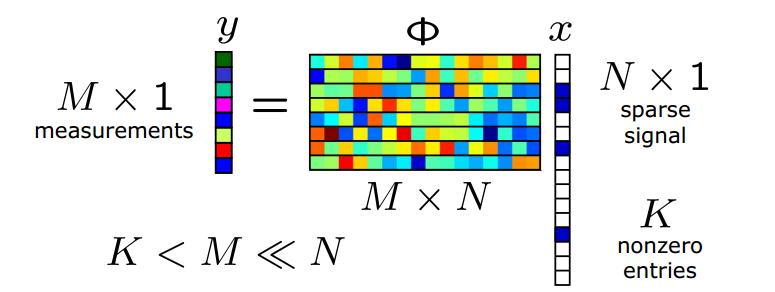
\includegraphics[height = 7 cm, width=\textwidth]{compressive_sensing_example.jpg}
\caption{A visualisation of the Compressive Sensing problem as an under-determined system}
\label{l1l2}
\end{figure*}


We may not be able to directly obtain these coefficients, as we may not posses an appropriate measuring device or one may not exist, or there is considerable uncertainty about where the non-zero coefficients are. Yet we still are able to measure correlations between the signal and some waveforms \(\psi_{k}\) i.e. 

\begin{equation}
y_{k} = \left\langle \alpha \text{,} \psi_{k} \right\rangle \text{ } k = 1 \ldots m
\end{equation}


Given a signal \(\alpha \in \re^n\), a matrix \(A \in \re^{m \times n}\), with \(m \ll n\),  we can acquire the signal via the set of linear measurements:

\begin{equation}
y = Ax
\end{equation}

where in this case \(A\) represents the sampling system (i.e the columns of \(A\) are the products of the two bases \(\psi\), \(\phi\)). In contrast to classical sensing, which requires that \(m = n\) for there to be no loss of information, it is possible to reconstruct \(x\) from an under-determined set of measurements as long as \(x\) is sparse in some basis. 

There are two conditions the matrix \(A\) needs to satisfy for recovery below Nyquist rates:

\begin{enumerate}
\item Restricted Isometry Property.
\item Incoherence between sensing and signal bases.
\end{enumerate}

\begin{definition}[RIP]\label{def:RIP}
We say that a matrix \(A\) satisifes the RIP of order \(s\) if there exists a \(\delta \in \left(0, 1\right)\) such that for all \(x \in \Sigma_s\):

\begin{equation}
\left(1 - \delta\right) \vectornorm{x}_2^2 \leq \vectornorm{Ax}_2^2 \leq \left(1 + \delta\right) \vectornorm{x}_2^2
\end{equation}
i.e. \(A\) approximately preserves the lengths of all \(s\)-sparse vectors in \(\re^n\). 
\label{def:RIP}
\end{definition}

\begin{remark}
Although the matrix \(A\) is not square, the RIP (\ref{def:RIP}) ensures that \(A^TA\) is close to the identity, and so \(A\) behaves approximately as if it were orthogonal. This is formalised in the following lemma from \cite{shalev2014understanding}:

\begin{lemma}
Let A be a matrix which satisfies the RIP of order 2\(s\) with RIP constant \(\delta\). Then for two disjoint subsets \(I, J \subset \left[n\right]\) each of size at most \(s\), and for any vector \(u \in \re^n\):

\begin{equation}
\langle Au_I, Au_J \rangle \leq \delta \vectornorm{u_I}_2^2 \vectornorm{u_J}_2^2
\end{equation}
\\
where \(u_I\) is the vector with component \(u_i\) if \(i \in I\) and zero elsewhere.

\end{lemma}

\end{remark}

\begin{remark} [Information Preservation]
A necessary condition to recover all \(s\)-sparse vectors from the measurements \(Ax\) is that \(Ax_1 \neq Ax_2\) for any pair \( x_ \neq x_2\), \(x_1, x_2 \in \Sigma_s\), which is equivalent to \(\vectornorm{A\left(x_1 - x_2\right)}_2^2 > 0\). 

This is guaranteed as long as \(A\) satisfies the RIP of order 2\(s\) with constant \(\delta\) - as the vector \(x_1 - x_2\) will hve at most \(2s\) non-zero entries, and so will be distinguishable after multiplication with \(A\). To complete the argument take \(x = x_1 - x_2\) in definition \eqref{def:RIP}, guaranteeing \(\vectornorm{A\left(x_1 - x_2\right)}_2^2 > 0 \), and requiring the RIP order of \(A\) to be \(2s\).
\end{remark}

\begin{remark} [Stability]
We also require that the dimensionality reduction of compressed sensing is the preservation of relative distances: that is if \(x_1\) and \(x_2\) are far apart in \(\re^n\) then their projections \(Ax_1\) and \(Ax_2\) are far apart in \(\re^m\). This will guarantee that the dimensionality reduction is robust to noise. 
\end{remark}

A requirement on the matrix \(A\) that satisfies both of these conditions is the following:

\begin{definition}[\(\delta\)-stable embedding]
We say that a mapping is a \(\delta\)-stable embedding of \(U,V \subset \re^n\) if

\begin{equation}
\left(1 - \delta \right) \vectornorm{u-v}_2^2 \leq \vectornorm{Au-Av}_2^2 \leq \left(1 + \delta\right) \vectornorm{u-v}_2^2
\end{equation}

for all \(u \in U\) and \(v \in V\). 
\label{def:d-stable}
\end{definition} 

\begin{remark}
Note that a matrix \(A\), satisfying the RIP of order \(2s\) is a \(\delta\)-stable embedding of \(\Sigma_s, \Sigma_s\). 
\end{remark}

\begin{remark}
Definition \ref{def:d-stable} has a simple interpretation: the matrix \(A\) must approximately preserve Euclidean distances between all points in the signal model \(\Sigma_s\).
\end{remark}

Given that we know a basis in which our signal is sparse, \(\phi\), how do we choose \(\psi\), so that we can accomplish this sensing task? In classical sensing, we choose \(\psi_k\) to be the set of \( T_s \)-spaced delta functions (or equivalently the set of \( 1/T_s \) spaced delta functions in the frequency domain). A simple set of \(\psi_k\) would be to choose a (random) subset of the delta functions above.

In general, we seek waveforms in which the signals' representation would be dense.

\begin{definition}[Incoherence]
A pair of bases is said to be incoherent if the largest projection of two elements between the sensing (\(\psi\)) and representation (\(\phi\)) basis  is in the set \( [1 , \sqrt{n}] \), where \( n \) is the dimension of the signal. The coherence of a set of bases is denoted by \(\mu\).
\end{definition}
Examples of pairs of incoherent bases are:

\begin{itemize}
\item Time and Fourier bases: Let \(\Phi = \textbf{I}_n\) be the canonical basis and \(\Psi = \textbf{F}\) with \(\psi_i = n^{-1\\2}e^{i\omega k} \) be the Fourier basis, then \(\mu\left(\phi, \psi\right) = 1\). This corresponds to the classical sampling strategy in time or space.
\item Consider the basis \(\Phi\) to have only entries in a single row, then the coherence between \(\Phi\) and any fixed basis \(\Psi\) will be \(\sqrt{n}\).
\item Random matrices are incoherent with any fixed basis \(\Psi\). We can choose \(\Phi\) by creating \(n\) orthonormal vectors from \(n\) vectors sampled independently and uniformly on the unit sphere. With high probability \(\mu = \sqrt{n\log{n}}\). This extends to matrices whose rows are created by sampling independent Gaussian or Bernoulli random vectors.
\end{itemize}

This implies that sensing with incoherent systems is good (in the sine wave example above it would be better to sample randomly in the time domain as opposed to the frequency domain), and efficient mechanisms ought to acquire correlations with random waveforms (e.g. white noise).

\textbf{Theorem} \cite{Candes2006}
Fix a signal f \(\in \mathbb{R}^n\) with a sparse coefficient basis, \(x_{i}\) in \(\phi\). Then a reconstruction from \(m\) random measurements in \(\psi\) is possible with probability \(1 - \delta\) if: 

\begin{equation}
m \geq C \mu^2(\phi, \psi) S \log\left(\frac{n}{\delta}\right)
\end{equation}
\label{minsamples}

where \( \mu(\phi, \psi)\) is the coherence of the two bases, and \(S\) is the number of non-zero entries on the support of the signal.

\subsection{Random Matrix Constructions} \label{sec:mtx-contruction}

To construct matrices satisfying definition \ref{def:d-stable}, given \(m, n\) we generate \(A\) by \(A_{ij}\) being i.i.d random variables from distributions with the following conditions \cite{davenport2010signal}

\begin{condition}[Norm preservation]
\(\ep A_{ij}^2 = \frac{1}{m}\)
\label{cond:norm-pres}
\end{condition}

\begin{condition}[sub-Gaussian]
\(\ep\left( e^{A_{ij}t} \right) \leq e^{C^2 t^2 /2}\)
\label{cond:sub-Gauss}
\end{condition}

Random variables \(A_{ij}\) satisfying conditions \eqref{cond:norm-pres} and \eqref{cond:sub-Gauss} satisfy the following concentration inequality \cite{baraniuk2008simple}:

\begin{lemma}[sub-Gaussian]
\begin{equation}
\pr\left( \mid \vectornorm{Ax}_2^2 - \vectornorm{x}_2^2 \mid \geq \varepsilon  \vectornorm{x}_2^2 \right) \leq 2e^{-cM\varepsilon^2}
\label{cond:sub-Gauss concetration}
\end{equation} 
\end{lemma}

Then in \cite{baraniuk2008simple} the following theorem is proved:

\begin{theorem}
Suppose that \(m\), \(n\) and \(0 < \delta < 1\) are given. If the probability distribution generating \(A\) satisfies condition \eqref{cond:sub-Gauss concetration}, then there exist constants \(c_1, c_2\) depending only on \(\delta\) such that the RIP \eqref{def:RIP} holds for \(A\) with the prescribed \(\delta\) and any  \(s \leq \frac{c_1 n}{\log{n/s}}\) with probability \(\geq 1-2e^{-c_2n}\) 
\end{theorem}

For example, if we take \(A_{ij} \sim \mathcal{N}\left(0, 1/m\right)\), then the matrix \(A\) will satisfy the RIP 

\subsection{Wishart Matrices}

Let \(\{X_i\}_{i=1}^r\) be a set of i.i.d \(1 \times p\) random vectors drawn from the multivariate normal distribution with mean 0 and covariance matrix \(H\).

\begin{equation}
X_i = \left(x_1^{(i)}, \ldots , x_p^{(i)}\right) \sim N\left(0, H\right)
\end{equation}

We form the matrix \(X\) by concatenating the \(r\) random vectors into a \(r \times p\) matrix.

\begin{definition}[Wishart Matrix]
Let 

\begin{equation}
W = \sum_{j=1}^r X_j X_j^T =  X X^T
\end{equation}

Then \(W \in \re^{r \times r}\) has the Wishart distribution with parameters 

\begin{equation}
W_r\left(H, p\right)
\end{equation}

where \(p\) is the number of degrees of freedom.
\end{definition}

\begin{remark}
This distribution is a generalisation of the Chi-squared distribution: let \(p = H = 1\). 
\end{remark}

\begin{theorem}[Expected Value]
\begin{equation}
\ep\left(W\right) = rH
\end{equation}
\end{theorem}
\begin{proof}
\begin{align*}
\ep\left(W\right) &= \ep\left(\sum_{j=1}^r X_j X_j^T\right) \\
&= \sum_{j=1}^r \ep\left(X_jX_j^T\right) \\
&= \sum_{j=1}^r \left( \mathrm{Var}(X_j) + \ep(X_j) \ep(X_j^T)   \right) \\
&= rH 
\end{align*}
Where the last line follows as \(X_j\) is drawn from a distribution with zero mean.
\end{proof}

\begin{remark}
The matrix \(M = A^TA\), where \(A\) is constructed by the methods from section \ref{sec:mtx-contruction}, will have a Wishart distribution. In particular, it will have \(\ep M = \frac{1}{m}I_n\) 
\label{remark: exp AtA}
\end{remark}

The joint distribution of the eigenvalues is given by \cite{levequeMatrices}:

\begin{equation}
p\left(\lambda_1, \ldots, \lambda_r\right) = c_r \prod_{i=1}^r e^{-\lambda_i}\prod_{i<j}\left(\lambda_i - \lambda_j\right)^2
\end{equation}

The eigenvectors are uniform on the unit sphere in \(\re^{r}\).

\subsection{Reconstruction Algorithms}
Compressive sensing places the computational load on reconstructing the Nyquist samples \(x\), from the set of compressive samples \(y\). This is in contrast to traditional sensing, where the heavy lifting computationally is done by the process with discretises the continuous signal to create the digital samples. 

Many recovery algorithms have been proposed, and all are based upon minimising some functional of the data. Generally, this is based upon two terms: a data fidelity term, minimising the discrepancy between the reconstruction and the true data, and regularisation term, biasing the reconstruction towards a class of solutions with desirable properties, for example sparsity. Typically the squared error \( \frac{1}{2}\vectornorm{y-Ax}_2^2 \) is chosen as the data fidelity term, whilst a number of regularisation terms have been introduced in the literature. 

A particularly important functional is:

\begin{equation}
\argmin_x \vectornorm{x}_1 \text{ s.t } y=Ax
\label{program:bp}
\end{equation}

known as Basis Pursuit \cite{Chen1998a}, with the following program known as the LASSO \cite{tibshirani1996regression} as a noisy generalisation: 

\begin{equation}
\argmin_x \frac{1}{2}\vectornorm{Ax-y}_2^2 + \lambda\vectornorm{x}_1
\label{program:lasso}
\end{equation}

The statistical properties of LASSO have been well studied. The program performs, both regularisation and variable selection: the parameter \(\lambda\) trades of data fidelity and sparsity with higher values of \(\lambda\) leading to sparser solutions. 

The LASSO shares several features with Ridge regression, and the Non-negative garotte (used for subset regression). It can be shown \cite{hastie2005elements}, that the solution to \eqref{program:lasso} can be written as:

\begin{equation}
\hat{x} = S_{\lambda}\left(x^{OLS}\right) = x^{OLS} \mathrm{sign}\left(x_i - \lambda\right)
\label{soln:lasso}
\end{equation} 

where \(x^{OLS} = (A^TA)^{-1}A^Ty \), whereas the solution to Ridge regression:

\begin{equation}
\argmin_x \frac{1}{2}\vectornorm{Ax-y}_2^2 + \lambda\vectornorm{x}_2^2
\label{program:ridge}
\end{equation}

can be written as:

\begin{equation}
\hat{x} = \left(1+\lambda\right)^{-1}x^{OLS}
\label{soln:ridge}
\end{equation}

and the solution to the best subset regression:

\begin{equation}
\argmin_x \frac{1}{2}\vectornorm{Ax-y}_2^2 + \lambda\vectornorm{x}_0
\label{program:ell0}
\end{equation}

where \( \vectornorm{x}_0 = \{ |i| : x_i \neq 0 \} \), can be written as:

\begin{equation}
\hat{x} = H_{\lambda}\left(x^{OLS}\right) = x^{OLS} \mathbb{I}\left(|x^{OLS}| > \lambda\right)
\label{soln:l0}
\end{equation} 

where \(\mathbb{I}\) is the indicator function. From \eqref{soln:l0} and \eqref{soln:ridge}, we can see that the solution to \eqref{program:lasso}, \eqref{soln:lasso}, translates coefficients towards zero by a constant factor, and set coefficients to zero if they are too small; thus the LASSO is able to perform both model selection (choosing relevant covariates) and regularisation (shrinking model coefficients). 

\begin{figure*}[h]
\centering
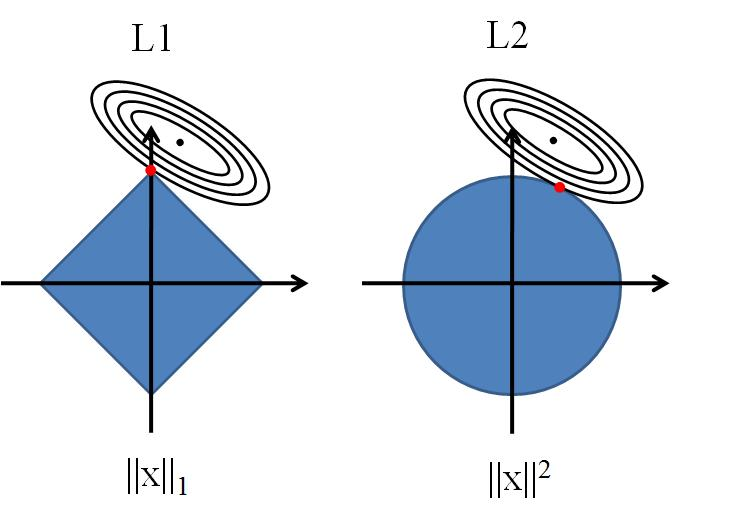
\includegraphics[height = 7 cm]{l1l2.jpg}
\caption{Solutions to the Compressive Sensing optimisation problem intersect the \(l_1\) norm the points where all components (but one) of the vector are zero (i.e. it is sparsity promoting) \cite{Tibshirani1996}}
\label{fig:l1l2}
\end{figure*}

Figure \eqref{fig:l1l2}, provides a graphical demonstration of why the LASSO promotes sparse solutions. \eqref{program:lasso} can also be thought of as the best convex approximation of the \(\ell_0\) problem \eqref{program:ell0}, as the \(\ell_1\)-norm is the convex hull of the points defined by \(\vectornorm{x}_p\) for \(p < 1\) as \(p \rightarrow 0\). 

%The representative algorithm for this type of minimisation is Basis-Pursuit . %

Other examples of regularisers are:

\begin{itemize}
\item Elastic Net: This estimator is a blend of both \eqref{program:lasso} and \eqref{program:lasso}, found by minimising:

\begin{equation}
\argmin_x \frac{1}{2}\vectornorm{Ax-y}_2^2 + \lambda\vectornorm{x}_2^2 + \mu\vectornorm{x}_1
\label{program:enat}
\end{equation}

The estimate has the benefits of both Ridge and Lasso regression: feature selection from the LASSO, and regularisation for numerical stability (useful in the under-determined case we consider here) from Ridge regression. The Elastic-net will outperform the LASSO when there is a high degree of collinearity between coefficients of the true solution.

\item TV regularisation

\begin{equation}
\argmin_x \frac{1}{2}\vectornorm{Ax-y}_2^2 +  \lambda\vectornorm{\nabla x}_1
\label{program:enat}
\end{equation}

This type of regularisation is used when preserving edges whilst simultaneously de-noising a signal is required. It is used extensively in image processing, where signals exhibit large flat patches alongside large discontinuities between groups of pixels.

\item Candes and Tao in \cite{candes2007dantzig}, propose an alternative  functional:

\begin{equation}
\min_{x \in \re^n} \vectornorm{x}_1 \text{ s.t. } \vectornorm{A^T(Ax-y)}_{\infty} \leq t\sigma
\end{equation}

with \(t = c\sqrt{2\log{n}}\). Similarly to the LASSO this functional selects sparse vectors consistent with the data, in the sense that the residual \(r = y - Ax\) is smaller than the maximum amount of noise present. In \cite{candes2007dantzig} it was shown that the \(l_2\) error of the solution is within a factor of \(\log{n}\) of the ideal \(l_2\) error. More recent work by Bikel, Ritov, and Tsybakov, \cite{bickel2009simultaneous}, has shown that the LASSO enjoys similar properties.
\end{itemize}

%Convex algorithms all relax the \(l\)-0 requirement for recovery \cite{tropp2006relax}, by instead solving the equivalent \(l\)-1 minimisation problem:%

Broadly reconstruction algorithms fall into three classes: convex-optimisations/linear programming, greedy methods, and Bayesian methods. Convex optimisation methods offer better performance, measured in terms of reconstruction accuracy, at the cost of greater computational complexity. Greedy methods are relatively simpler, but don't have the reconstruction guarantees of convex algorithms. Bayesian methods offer the best reconstruction guarantees, as well as uncertainty estimates about the quality of reconstruction, but come with considerable computational complexity.

A recent greedy method, Approximate Message Passing (AMP), is a blend of both greedy and Bayesian methods \cite{donoho2009message}.

Convex methods cast the optimisation objective either as a linear program with linear constraints, or as a second order cone program with quadratic constraints. Both of these types of program can be solved with first order interior point methods. However, their practical application to compressive sensing problems is limited due to their polynomial dependence upon the signal dimension and the number of constraints. 

Compressive Sensing poses a few difficulties for convex optimisation based methods. In particular, many of the unconstrained objectives are non-smooth meaning methods based upon descent down a smooth gradient are inapplicable. 

To overcome these difficulties, a series of algorithms originally proposed for wavelet-based image de-noising have been applied to CS, known as iterative shrinkage methods. These have the desirable property that they boil down to matrix-vector multiplications and component-wise thresholding.

Iterative shrinkage algorithms replace searching for a minimal facet of a complex polytope by a iteratively denoised gradient descent. The choice of the (component-wise) denoiser is dependent upon the regulaiser used in \ref{program:lasso}. These algorithms have an interpretation as Expectation-Maximisation \cite{figueiredo2003algorithm} - where the E-step is performed as gradient descent, and the M-step is the application of the denoiser.

\begin{figure}
\begin{algorithmic}[1]
\Procedure{IST}{$y,A, \mu, \tau, \varepsilon$}
\State $x^0 = 0$
\While{$\vectornorm{x^{t} - x^{t-1}}_2^2 \leq \varepsilon$}
\State $x^{t+1} \gets S_{\mu\tau}\left(x^t + \tau A^Tz^t \right) $
\State $z^t \gets y - Ax^t$
\EndWhile
\State \textbf{return} $x^{t+1}$
\EndProcedure
\end{algorithmic}
\caption{The Iterative Soft Thresholding Algorithm}\label{alg:IST}
\end{figure}

%There has been a line of work on algorithms directly minimising the \(l\)-0 norm \cite{wen2015efficient}, \cite{oxvig2012improving}, \cite{mohimani2010sparse}.

Greedy methods are another family of solutions to \ref{program:lasso}. They offer reduced computational complexity with correspondingly worse reconstruction quality and poorer guarantees on sparsity and undersampling than convex algorithms. Examples of this type are Orthogonal Matching Pursuit (OMP)\cite{tropp2007signal}, and Compressive Sensing Orthogonal Matching Pursuit (CoSAMP). 


\begin{figure}
\begin{algorithmic}[1]
\Procedure{OMP}{$y,A,K,\varepsilon$}
\State $x^0 = 0$, $r=y$, $\Omega = \varnothing$, $i=0$
\While{$\vectornorm{x^{t} - x^{t-1}}_2^2 \leq \varepsilon$}
\State $i \gets i+1$
\State $b\gets A^Tr$
\State $\Omega \gets \Omega \cup \mathrm{supp}\left(H_1\left(b\right)\right)$
\State $x\restriction_{\Omega} \gets A^T\restriction_{\Omega}x$
\State $x\restriction_{\Omega^c} \gets 0$
\State $b \gets y - Ax$
\EndWhile
\State \textbf{return} $x$
\EndProcedure
\end{algorithmic}
\caption{The OMP recovery algorithm}\label{alg:omp}
\end{figure}

The Greedy family of algorithms abandons exhaustive searches of the solution space in favour of locally optimal single term updates. They proceed by approximating the solution by some active set of columns from the sensinng matrix \(A\) and solving a restricted least-squares problem at each (in the case of OMP). This guarantees a maximal reduction in \(l\)-2 error in each iteration.

Despite their computational simplicity, greedy algorithms have several drawbacks. Primarily they do not come with stable recovery guarantees, and they require a larger number of samples to recover the signal when compared to Bayesian and Convex recovery algorithms. Also, due to their greedy nature, these algorithms are not guaranteed to converge: in fact it can be shown that there exist \(k\)-sparse vectors and sensing matrices \(A\) such that OMP fails to converge in k iterations \cite{wen2013improved}.



\begin{figure}
\begin{algorithmic}[1]
\Procedure{AMP}{$y,A,\varepsilon$}
\State $x^0 = 0$, $z^0=A^Ty$
\While{$\vectornorm{x^{t} - x^{t-1}}_2^2 \leq \varepsilon$}
\State $x^{t+1} \gets S_{\mu\tau}\left(x^t - \tau+ A^Tz^t\right) $
\State $z^{t+1} \gets y - Ax^t + \frac{\vectornorm{x}_0}{m}z^t$
\EndWhile
\State \textbf{return} $x^{t+1}$
\EndProcedure
\end{algorithmic}
\caption{The AMP recovery algorithm}\label{alg:amp}
\end{figure}



Bayesian methods reformulate the optimisation problem into an inference problem. These methods come with a unified theory, and standard methods to produce solutions. The theory is able to handle hyper-parameters in a unified way, provides a flexible modelling framework, and is able to provide desirable statistical quantities such as the uncertainty inherent in the prediction.

Based on the discussion above we can represent the compressive sensing measurements as: 

\begin{equation}
y = Ax
\end{equation}

where \(A\) is a \(K \times	N\) matrix which is the product of the measurement and sparse bases described earlier.

Note that the measurements may be noisy, with the measurement noise represented by a zero mean Gaussian distribution and unknown variance \( \sigma^2 \):

\begin{equation}
y = Ax + n
\end{equation}
\label{CSequation}

Where \textbf{n} is the vector representing the vector of noise, and has the same support as the measurements. 

Previous sections have shown how the weights \(x\) may be found through optimisation methods such as basis pursuit or greedy algorithms. Here, an alternative Bayesian model is described.

From \ref{CSequation} we have a Gaussian likelihood model: 

\begin{equation}
p \left(y \mid z\text{,} \sigma^2 \right) = (2 \pi \sigma^2)^{-K/2} \exp{\left(- \frac{1}{2 \sigma^2} \|y - Ax|_{2}^{2} \right)} 
\end{equation}

The above has converted the CS problem of inverting sparse weight \textbf{w} into a linear regression problem with a constraint (prior) that \textbf{w} is sparse. 

To seek the full posterior distribution over \textbf{w} and \( \sigma^2 \), we can chose a sparsity promoting prior. A popular sparseness prior is the Laplace density functions:

\begin{equation}
p\left(x\mid\lambda\right) = \left(\frac{\lambda}{2}\right)^N exp{-\lambda \sum_{i=1}^{N} |x_i|}
\end{equation}

Note that the solution the convex optimisation problem \ref{program0} corresponds to a maximum \textit{a posteriori} estimate for \(w\) using this prior. I.e this prior is equivalent to using the \(l_1\) norm as an optimisation function (see figure \ref{laplacenormal} \cite{Tibshirani1996}).

\begin{figure*}[h]
\centering
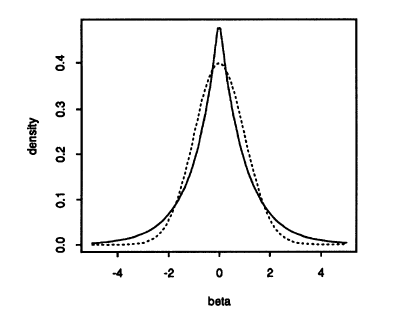
\includegraphics[height = 7 cm]{LaplaceandNormalDensity.png}
\caption{The Laplace (\(l_1\)-norm, bold line) and Normal (\(l_2\)-norm, dotted line) densities. Note that the Laplace density is sparsity promoting as it penalises solutions away from zero more than the Gaussian density. \cite{Tibshirani1996}}
\label{laplacenormal}
\end{figure*}

The full posterior distribution on \(w\) and \(\sigma^2\) may be realised, by using a hierarchical prior instead. To do this, define a zero-mean Gaussian prior on each element of \(w\):
%
\begin{equation}
p\left(w\mid a\right) = \prod_{i=1}^{N}\mathbb{N}\left(w_i\mid 0, \alpha_{i}^-1\right)
\end{equation}
%
where \(\alpha\) is the precision of the distribution. A gamma prior is then imposed on \(\alpha\):

\begin{equation}
p\left(\alpha \mid a, b \right) = \prod_{i=1}^{N} \Gamma\left( \alpha_i \mid a, b \right)
\end{equation}

The overall prior is found by marginalising over the hyperparameters:

\begin{equation}
p\left( w \mid a, b \right) = \prod_{i=1}^{N} \int_{0}^{\infty} \mathbb{N}\left(w_i\mid 0, \alpha_{i}^-1\right) \Gamma\left( \alpha_i \mid a, b \right)
\end{equation}

This integral can be done analytically and is a Student-t distribution. Choosing the parameters \(a,b\) appropriately we can make the Student-t distribution peak strongly around \(w_i = 0\) i.e. sparsifying. This process can be repeated for the noise variance \(\sigma^2\). The hierarchical model for this process is shown in \ref{bayesiancs}. This model, and other CS models which not necessarily have closed form solutions, can be solved via belief-propagation \cite{Baron2010}, or via Monte-Carlo methods.

\begin{figure*}[h]
\centering
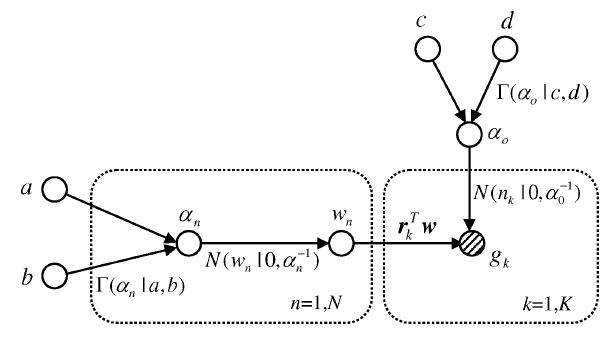
\includegraphics[height = 7 cm]{bayesiancs.png}
\caption{The hierarchical model for the Bayesian CS formulation \cite{Ji2008}}
\label{bayesiancs}
\end{figure*}

However, as with all methodologies, Bayesian algorithms have their drawbacks. Most notable is the use of the most computationally complex recovery algorithms. In particular MCMC methods suffer in high dimensional settings, such as those considered in compressive sensing. There has been an active line of work to address this: most notably Hamiltonian Monte Carlo - an MCMC sampling method designed to follow the typical set of the posterior density. 

Belief propagation (BP) \cite{Yedidia2011} is a popular iterative algorithm, offering improved reconstruction quality and undersampling performance. However, it is a computationally complex algorithm. It is also difficult to implement. Approximate message passing \eqref{alg:amp} solves this issue by blending BP and (IT).

The algorithm proceeds like iterative thresholding, but computes an adjusted residual at each stage. The extra term comes from a first order approximation to the messages passed by BP \cite{metzler2014denoising}.

The choice of prior is key in Bayesian inference, as it encodes all knowledge about the problem. Penalising the least-squares estimate  with the \(\ell_1\) norm, has a Bayesian interpretation as a Laplace distribution prior. This is distinct from the LASSO however, as this Bayesian model does not set coefficients to zero exactly - instead it sets many coefficients to be small. Other priors have been suggested in the literature, such as the Horseshoe  prior, which do set covariates to zero. These do not have the desirable property of leading to closed form posteriors (as shown above).

\section{Compressive Sensing Architechtures}\label{sec:sensingmodel}

\subsection{Modulated Wideband Converter}
We consider a radio environment with a single primary user (PU) and a network of \(J\) nodes collaboratively trying to sense and reconstruct the PU signal, either in a fully distributed manner (by local communication), or by transmitting measurements to a fusion centre which then solves the linear system. 

We try to sense and reconstruct a wideband signal, divided into \(L\) channels. We have a (connected) network of \(J\) (= 50) nodes placed uniformly at random within the square \(  \left[0,1\right]\times \left[0,1\right] \). This is the same model, as in \cite{Zhang2011b}. The calculations which follow are taken from \cite{Zhang2011b} as well.

The nodes individually take measurements (as in \cite{mishali2010theory}) by mixing the incoming analogue signal \(x\left(t\right)\) with a mixing function \(p_i\left(t\right)\) aliasing the spectrum. \(x\left(t\right)\) is assumed to be bandlimited and composed of up to \(k\) uncorrelated transmissions over the \(L\) possible narrowband channels - i.e. the signal is \(k\)-sparse. 

\begin{figure}[h]
\centering
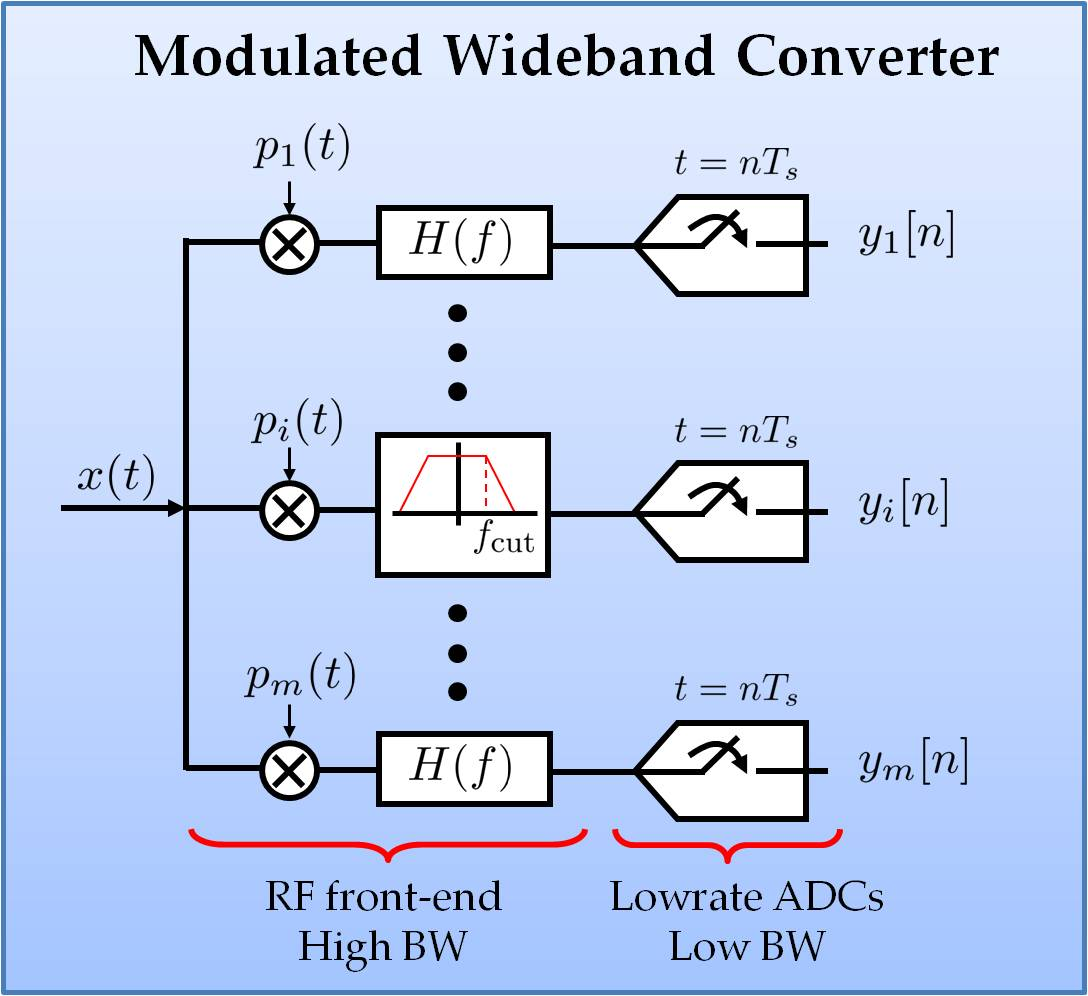
\includegraphics[height = 7.3 cm]{Modulated_wideband_converter.jpg}
\caption{Mse vs SNR for the sensing model, with AWGN only, showing the performance of distributed and centralised solvers}
\label{msevssnr0}
\end{figure}

The mixing functions - which are independent for each node - are required to be periodic, with period \(T_p\). Since \(p_i\) is periodic it has Fourier expansion:

\begin{equation}
p_i\left(t\right) = \sum_{l=-\infty}^{\infty} c_{il} \exp\left({jlt\frac{2\pi}{T_p}}\right)
\end{equation}

The \(c_{il}\) are the Fourier coefficients of the expansion and are defined in the standard manner. The result of the mixing procedure in channel \(i\) is therefore the product \(xp_i\), with Fourier transform (we denote the Fourier Transform of \(x\) by \(X\left( \dot{.} \right)\)):

\begin{align}
X_{i}\left(f\right) &=& \int_{-\infty}^{\infty} x\left(t\right) p_i\left(t\right) dt \nonumber
\\ &=& \sum_{l=-\infty}^{\infty} c_{il} X\left(f-lf_p\right)
\end{align}

(We insert the Fourier series for \(p_i\), then exchange the sum and integral). The output of this mixing process then, is a linear combination of shifted copies of \(X\left(f\right)\), with at most \(\lceil f_NYQ/f_p\rceil\) terms since \(X\left(f\right)\) is zero outside its support (we have assumed this Nyquist frequency exists, even though we never sample at that rate).

This process is repeated in parallel at each node so that each band in \(x\) appears in baseband.

Once the mixing process has been completed the signal in each channel is low-pass filtered and sampled at a rate \(f_s \geq f_p\). In the frequency domain this is a ideal rectangle function, so the output of a single channel is:

\begin{equation}
Y_i\left(e^{j 2 \pi f T_s }\right) = \sum_{l = -L_0}^{+L_0} c_{il} X\left(f-lf_p\right)
\end{equation}

since frequencies outside of \([-f_s/2, f_s/2]\) will filtered out. \(L_0\) is the smallest integer number of non-zero contributions in \(X\left(f\right)\) over \([-f_s/2, f_s/2]\) - at most \(\lceil f_NYQ/f_p\rceil\) if we choose \(f_s = f_p\). These relations can be written in matrix form as:

\begin{equation}
\textbf{y} = \textbf{A}\textbf{x} + \vec{w}
\label{system}
\end{equation}

where \(\textbf{y}\) contains the output of the measurement process, and \(\textbf{A}\) is a product matrix of the mixing functions, their Fourier coefficients, a partial Fourier Matrix, and a matrix of channel coefficients. \(\textbf{x}\) is the vector of unknown samples of \(x\left(t\right)\). 

i.e. \(\textbf{A}\) can be written: 

\begin{equation}
\textbf{A}^{m\times L} = \textbf{S}^{m\times L} \textbf{F}^{L\times L} \textbf{D}^{L \times L} \textbf{H}^{L \times L}
\end{equation}

The system  \ref{system} can then be solved (in the sense of finding the sparse vector \(\vec{x}\) by convex optimisation via minimising the objective function:

\begin{equation}
\frac{1}{2}\|\textbf{Ax}-\textbf{y}\|_2^2 + \lambda \|\textbf{x}\|_1
\end{equation}

where \(\lambda\) is a parameter chosen to promote sparsity. Larger \(\lambda\) means sparser \(\vec{x}\).

\subsection{Random Demodulator}
We assume that the analogue signal \(x\left(t\right)\) is comprised of a finite number of components from some arbitrary dictionary \(\psi_n\left(t\right)\):

\begin{equation}
x\left(t\right) = \sum_{n=1}^N \alpha_n \psi_n\left(t\right)
\end{equation}

The signal is said to be sparse when there are only a few non-zero \(\alpha_n\). The dictionary elements \(\psi_n\) may have a relatively high bandwidth, but the signal itself will have only a few degrees of freedom.

The signal acquisition method proposed consists of three stages (all analogue processing): demodulation, filtering and uniform sampling. 

Initially, the signal is modulated by a pseudo-random sequence \(p_c\left(t\right)\), which alternates at frequencies at (or above) the Nyquist frequency of \(x\left(t\right)\). The signal is then filtered, through a filter with impulse response \(h\left(t\right)\), before being sampled at rate \(\mathcal{M}\) with a traditional ADC.

The output of this system, \(y\left[m\right]\), can be related to the input \(x\left(t\right)\) via a linear transformation of the coefficient vector \(\alpha_n\). 

To find the transformation \(A\), first consider the output of \(y\left[m\right]\), which is the result of convolution and demodulation followed by sampling at rate \(\mathcal{M}\):

\begin{equation}
y\left[m\right] = \int_{-\infty}^{\infty} x\left(\tau\right)p_c\left(\tau\right)h\left(t - \tau\right)\mid_{t = m\mathcal{M}}d\tau
\end{equation}

and by expanding \(x\left(t\right) = \sum_{n=1}^N \alpha_n \psi_n\left(t\right)\):

\begin{equation}
y\left[m\right] =  \sum_{n=1}^N \alpha_n \int_{-\infty}^{\infty} \psi_n\left(t\right)p_c\left(\tau\right)h\left(m\mathcal{M} - \tau\right)d\tau
\end{equation}

we see that the output can be written as:

\begin{equation}
y = Ax
\end{equation}

with

\begin{equation}
A_{m,n} = \int_{-\infty}^{\infty} \psi_n\left(t\right)p_c\left(\tau\right)h\left(m\mathcal{M} - \tau\right)d\tau
\end{equation}

\bibliography{thesis}

\end{document}

\chapter{ADMM}
\section{Introduction}\label{chap:admm}

This chapter surveys the Alternating Direction Method of Multipliers (ADMM). This is an efficient convex algorithm for inference in high dimensional problems and can be applied to inverting the compressive samples, producing accurate estimates of the original signal. 

We begin (in section \ref{sec:admm}) by introducing the algorithm, the type of problem for which it is an appropriate tool, and the algorithm's history. In particular we make connections with MAP estimation in high dimensional statistics. We discuss two worked examples: finding the minimal norm solution of a set of linear equations, and the Least Absolute Shrinkage and Selection Operator. The first example is to give a simple introduction to ADMM via a well known result, whilst the second is particularly relevant to compressive sensing. 

In section \ref{sec:prox}, we move on from the examples, to a more advanced discussion where we formalise the proximity operator. The Prox operator is a generalisation of the Euclidean projection, and can be evaluated for a variety of common optimisation objectives. The evaluation is either directly in closed form, or via a simple to evaluate component-wise algorithm. The proximity operator moves the objective in the direction of the minimiser, and thus can be thought of a generalisation of gradient descent. We show some examples of how to compute the proximity operator, for functions which appear in statistical estimation. We also show its connection to ADMM - the algorithm proceeds by iteratively computing the Prox operators (see definition \eqref{def:prox_operator}) of the two functions comprising the objective. This is why it is such an useful algorithm: if the relevant proximity operators are easy to evaluate, then ADMM is an inexpensive and relatively fast algorithm.

Finally, we discuss acceleration techniques for ADMM, in section \ref{sec:accel}. In particular, we discuss schemes by Nesterov for non-smooth functions. We show that generalised gradient descent can be thought of as constructing an approximating polynomial to the objective term by term. By considering Chebyshev polynomials, we can improve the speed of approximation accuracy and that this is the reason that Nesterov acceleration works.

\section{Background}\label{sec:admm}

We begin this section with some definiitions, pinning down the kind of functions we will be optimising over (closed, proper, convex functions with Lipschitz continuous gradients). We then discuss the Lagrangian formulation of constrained optimisation, discussing some precursers to ADMM. Finally the algorithm is introduced and explained.

\subsection{Preliminary Definitiona}

\begin{definition}[Convexity]
We say that a function \(f\) is \textbf{convex} is it satisfies the following inequality:

\begin{equation}
f\left(\lambda x_1 + \left(1-\lambda\right)x_2\right) \leq \lambda f\left(x_1\right) + \left(1-\lambda\right) f\left(x_2\right)
\end{equation}

This can be rephrased as:

\begin{equation}
f\left(\ep{x}\right) \leq \ep{f\left(x\right)}
\end{equation}

An intuitive physical metaphor for convexity can be found in MacKay \cite{mackay2003information}: if a collection of masses \(x_i\) are placed on a convex curve \(f\), then the centre of gravity of those masses, which lies at \(\left(\ep{x}, \ep{f\left(x\right)}\right)\) lies above the curve.

An equivalent definition of convextiy is that the Hessian (matrix of second derivatives of \(f\)) is positive definite (has only positive eigenvalues).
\end{definition}

A slightly stronger condition is that of strong convexity:

\begin{definition}[Strong convexity]
A function \(f: \re^n \rightarrow \re\) is said to be \(l\)-strongly convex if for some \(l > 0\) it satisfies:

\begin{equation}
f\left(y\right) \geq f\left(x\right) + \nabla f\left(x\right)^T \left(y-x\right) + \frac{l}{2}\vectornorm{x-y}^2
\end{equation}

\end{definition}

\begin{definition}[Closed function]
A function \(f: \re^n \rightarrow \re\) is said to be \textbf{closed} if \(\forall \alpha\) the sublevel set

\begin{equation}
\{x \in \mathrm{dom} f \mid f\left(x\right)\leq \alpha\}
\end{equation}

is closed

\end{definition}

\begin{definition}[Proper function]
A function \(f\) is said to be \textbf{proper}, if \(f\) has the property  that\(f\left(x\right) < \infty\) for at least one \(x\) and \(f\left(x\right)>-\infty\) for all \(x\).
\end{definition}

\begin{definition}[Closed, Proper convex function]
A function is said to be a \textbf{closed, proper convex function} is it is convex, proper and closed.
\end{definition}

\begin{example}
The function:
\begin{equation}
f\left(x\right) = c x^2
\end{equation}

on \([-1, 1]\) is a closed, proper, convex function. 
\end{example}

In this thesis the type of functions we are minimising, are closed, proper convex with Lipschitz continuous gradients. 

\begin{definition}
A function is said to have \textbf{Lipschitz continuous gradients} if its derivative satisfies:
\begin{equation}
\vectornorm{\nabla f\left(x\right) - \nabla f\left(y\right)} \leq L \vectornorm{x - y}
\end{equation}

\end{definition}

We will make use of the following definitions in passing in the following text, so it is useful to have them here:

\begin{definition}[Convex conjugate]

The function \(f^*: \re^n \rightarrow \re\) is the \textbf{convex conjugate} of the function \(f: \re^n \rightarrow \re\) where:

\begin{equation}
f^*\left(y\right) = \sup_{x \in \mathrm{dom} f} \left(y^Tx - f\left(x\right)\right)
\end{equation}

\end{definition}

and finally we define the condition number of \(f\):

\begin{definition}[Condition number]
The \textbf{condition number} of a closed, proper, and convex function \(f\) is defined to be:

\begin{equation}
\kappa = \frac{L}{l}
\end{equation}

where \(L\) is the Lipchitz constant, and \(l\) is the strong convexity constant.

\end{definition}

\subsection{Lagrangian Formulation}
\begin{definition}[Lagrangian]
In constrained optimisation, where a smooth function is minimised subject to constraints:

\begin{eqnarray}
\min_x f\left(x\right) \\
\text{s.t } g\left(x\right) = b
\end{eqnarray}

we define the Lagrangian to be the function:

\begin{equation}
L\left(x, \eta\right) = f\left(x\right) + \eta^T\left(b-g\left(x\right)\right)
\end{equation}

The variable \(x\) is refereed to as the primal variable.

\end{definition}

\begin{definition}[Lagrange Dual]
The Lagrange dual function is defined to be:

\begin{equation}
H\left(\eta\right) = \inf_x L\left(x, \eta\right)
\end{equation}

\end{definition}

\begin{definition}[Lagrange Multiplier]
The Lagrange multiplier \(\eta\) is defined as:

\begin{equation}
\frac{\partial L}{\partial b} = \eta
\end{equation}

That is the Lagrange multiplier is the rate of change of the quantity being optimised as a function of the constraint parameter.

\end{definition}

\begin{example}[One dimensional contrained optimisation \cite{Boyd2010a}]
For the minimisation problem 

\begin{eqnarray}
\min_x f\left(x\right) \\
\text{s.t } Ax = b
\end{eqnarray}

The Lagrangian is:

\begin{equation}
L\left(x, \eta\right) = f\left(x\right) + \eta^T\left(Ax - b\right)
\end{equation}

and the dual function is:

\begin{equation}
H\left(\eta\right) = -f^*\left(-A^T\eta\right) = b^Ty
\end{equation}

where \(f^*\) is the convex conjugate of \(f\).

\end{example}



\begin{example}[Dual Ascent]

For the minimisation problem 

\begin{eqnarray}
\min_x f\left(x\right) \\
\text{s.t } Ax = b
\end{eqnarray}

The Lagrangian is:

\begin{equation}
L\left(x, \eta\right) = f\left(x\right) + \eta^T\left(Ax - b\right)
\end{equation}

and the dual function is:

\begin{equation}
H\left(\eta\right) = -f^*\left(-A^T\eta\right) = b^Ty
\end{equation}

where \(f^*\) is the convex conjugate of \(f\).

The dual problem is:

\begin{equation}
\max_{\eta} H\left(\eta\right)
\end{equation}

We can find an optimum pair of points by gradient ascent. First we find a point \(x^+ = \argmin_x L\), and then we have \(\nabla g = Ax^+ - b\), which is the residual for the equality constraint. The dual ascent method is:

\begin{align}
x^{k+1} &:= \argmin_x L\\
\eta^{k+1} &:= \eta^{k} + \alpha \left(Ax^{k+1} -b \right)
\label{dual-ascent}
\end{align}

where \(\alpha\) is a step size.

The \(\eta\) variable can be interpreted as a vector of prices, that an agent must pay in order to satisfy the optimisation problem. Thus the second step in dual ascent (and the final step in ADMM) can be interpreted as a price update.

\end{example}

\subsection{ADMM}
ADMM is a convex optimisation algorithm which splits large, and typically non-smooth, problems into smaller pieces which are easier to handle. At heart, the algorithm involves finding a zero of a convex objective function, by evaluating proximal operators \cite{parikh2014proximal}, see definition \ref{def:prox_operator}. 

ADMM has a long history, first being investigated by Rockarfellar \cite{rockafellar1976monotone}, in the context of minimisation in Hilbert spaces - finite and infinite dimensional vector spaces equipped with an inner product and a metric induced by the inner product, typical examples include \(\re^n\), the space of \(n\)-dimensional Euclidean vectors, and \(\mathbb{L}^2\left(\re\right)\), the space of square-integrable functions over the reals. Douglas and Rachford \cite{douglas1956numerical} also investigated ADMM as a method for solving the heat equation. Subsequently the theory was generalised and extended by Eckstein and Bersekas \cite{eckstein1992douglas}.

ADMM has found applications in Sparse Coding \cite{Bristow2014}, Compressive Radar Imaging \cite{heredia2015consensus}, Medical Imaging \cite{sawatzky2014proximal}, and Optimal Control \cite{o2013splitting}. This is because many optimisation objective functions can be formulated as a sum of simpler convex functions, and casting the problem in an alternating minimisation framework is straightforward for practitioners.

ADMM also has explicit convergence rates, 
(see \cite{Shi2013}, and \cite{nishihara2015general}), which both show (through different methods), that in every step of the algorithm, the iterates moves towards the optimum by a factor of \(1-1/k\), where \(k\) is iteration number.

ADMM as lo has well understood methodologies for tuning and acceleration, \cite{ghadimi2015optimal} shows how to choose optimal step-sizes from  and \cite{goldstein2014fast} extends the algorithm to an accelerated version and gives quantitative guarantees on the convergence properties. 

However, care must be taken when the problem is posed as the sum of more than two convex functions - the direct extension is not necessarily convergent: the paper of Chen\cite{chen2016direct}, shows that ADMM applied to the sum of three functions will not necessarily converge.

ADMM is concerned with minimising a the sum of two functions, subject to a constraint:

\begin{align}
\argmin_{x} f\left( x \right) + g\left(z\right) \nonumber
\\
\text{s.t } Ux + Vz = c
\label{admm}
\end{align}

where \(f\) and \(g\) are assumed to be convex functions with range in \(\re\), \(U \in \re^{p \times n}\) and \(V\in \re^{p \times m}\) are matrices (not assumed to have full rank), and \(c \in \re^p\).

ADMM consists of iteratively minimising the augmented Lagrangian 

\begin{align*}
L_p\left(x, z, \eta\right) = f\left( x\right) +& g\left(z\right)+\eta^T\left(Ux+Vz-c\right) + \frac{\rho}{2}\|Ux+Vz-c\|_2^2
\label{admm_aug_lagrangian}
\end{align*}

where, \(x,z\) are the primal variables, \(\eta\) is a Lagrange multiplier (or dual variable), and \(\rho\) is a parameter we can choose to make \(g(z)\) smooth \cite{nesterov2005smooth}.

To perform the minimisation of the Lagrangian we use the following iterations:

\begin{align}
x^{k+1} &:= \argmin_{x} L_\rho\left(x,z^k,\eta^k\right)\\
z^{k+1} &:= \argmin_{z} L_\rho\left(x^{k+1},z,\eta^k\right)\\
\eta^{k+1} &:= \eta^{k} + \rho \left(Ux^{k+1} + Vz^{k+1} - c\right)
\label{admm_algo}
\end{align}

The first two steps are primal variable updates, and the second step is a dual variable update. We illustrate this second step again with a one dimensional example:

The alternating minimisation works because of the decomposability of the objective function: the \(x\) minimisation step is independent of the \(z\) minimisation step and vice versa.  

\begin{example}[Minimum norm solution of a Linear Equation]
Consider the following problem, of finding the minimum norm solution of a linear system:

\begin{eqnarray}
\min_x \vectornorm{x}_2\\
\text{s.t } Ax = y
\end{eqnarray}

where \(x \in \re^n\), \(y \in \re^n\), \(A \in \re^{n \times n}\) and we implicitly assume that \( y = Ax\) has a solution and that \(y\) is in the range of \(A\). 

This problem has the well known optimal solution:

\begin{equation}
x^{\star} = A^T \left(AA^T\right)^{-1}y
\end{equation}

This problem can be formulated as

\begin{eqnarray}
\min_x \vectornorm{x}_2 + \mathbb{I}\left(y\right) \\
\text{s.t } Ax - y = 0
\end{eqnarray}

The Lagrangian for this example, is then:

\begin{align*}
L_p\left(x, y, \eta\right) = \vectornorm{x}_2 + \mathbb{I}\left(y\right)+\eta^T\left(Ax-y\right) + \frac{\rho}{2}\vectornorm{Ax-y}_2^2
\label{minl2_aug_lagrangian}
\end{align*}

and the ADMM iterations are:

\begin{align}
x^{k+1} &:= \left(1-\frac{\rho}{\vectornorm{x^{k}}_2}\right)x^{k}\\
z^{k+1} &:= \Pi\left(x^{k+1}\right)\\
\eta^{k+1} &:= \eta^{k} + \rho \left(Ax^{k+1} + y^{k+1}\right)
\label{minl2_algo}
\end{align}
\end{example}

We now illustrate the theory with a more involved example, the LASSO.

\begin{example}[LASSO]
Given a set of measurements of the form

\begin{equation}
y = Ax + n 
\end{equation}

where \(x \in \re^n\) is an \(s\)-sparse vector we wish to recover, \(y \in \re^m\) is a set of noisy measurements, \(A \in \re^{m \times n}\) is a design or measurement matrix such that \(x\) is not in the null-space of \(A\), and \(z \in \re^m\) is AGWN. The signal \(x\) can be recovered by  minimising the objective function:

\begin{equation}
L = \frac{1}{2} \vectornorm{Ax-y}_2^2 + \lambda\vectornorm{x}_1
\label{LASSO}
\end{equation}

where \(\lambda\) is a parameter which trades off the reconstruction accuracy and sparsity of \(x\): larger \(\lambda\) means sparser \(x\). 

We also consider the problem:

\begin{equation}
L = \frac{1}{2} \vectornorm{Ax-y}_2^2 + \lambda\vectornorm{x}_0
\label{LASSO-L0}
\end{equation}

where \( \vectornorm{t}_0 = \{ |t| \mid t_i \neq 0 \} \).

The ADMM iterations for LASSO, which can be found by alternately differentiating \eqref{eq:lasso-lagrangian} with respect to \(x\),\(z\) and \(\eta\), are (in closed form):

\begin{align}
x^{k+1} &:= \left(A^TA + \rho I\right)^{-1}\left(A^Ty +\rho\left( z^k - \eta^k/\rho\right)\right)\\
z^{k+1} &:= S_{\lambda/\rho}\left(x^{k+1} + \eta^k/\rho\right)
 \\
\eta^{k+1} &:= \eta^{k} + \rho\left(x^{k+1}-z^{k+1}\right)
\label{admm_algo_lasso}
\end{align}

where \(S_{\lambda/\rho}\left(\circ\right)\) is the soft thresholding operator: \(S_\gamma\left(x\right)_i = \mathrm{sign}(x_i)\left(|x_i| - \gamma\right)^+\).

The individual steps in \eqref{admm_algo_lasso} can be found differentiating \eqref{eq:lasso-lagrangian} with respect to \(x\) and \(z\) as follows:

\begin{align*}
\frac{\partial L}{\partial x } = -A^T\left(y-Ax\right) + \rho (x-z) + \eta
\end{align*}

as 

\begin{equation}
\frac{\partial}{\partial x} \vectornorm{F(x)}_2^2 = 2\left(\frac{\partial}{\partial x} F(x)\right) F(x) 
\label{dellx}
\end{equation}

by the chain rule, and \(\partial/\partial x (Ax) = -A^T\) (see the Matrix Cookbook, \cite{petersen2008matrix}) as differentiation exchanges a linear operator with its adjoint.

Setting \eqref{dellx} to zero and collecting like terms:

\begin{equation}
\left(A^TA + \rho I\right)x = A^Ty + \rho z - \eta
\end{equation}

so we find the optimal \(x\) is:

\begin{equation}
x = \left(A^T A + \rho I\right)^{-1}\left(A^Ty + \rho \left( z - \eta/\rho\right)\right)
\label{optx}
\end{equation}

note that this estimator is a weighted average of the ordinary least squares estimate (\(A^Ty\)) and a Gaussian prior. This is to be expected, as the minimisation problem w.r.t x is an \(l_2\)-regularised MAP problem.

for \(z > 0\)

\begin{equation}
\frac{\partial L} {\partial z} = \lambda + \rho (x-z) - \eta
\label{dellz-positive}
\end{equation}

from which we obtain:

\begin{equation*}
z = x + \frac{1}{\rho} ( \eta - \lambda )
\end{equation*}

since \(z>0\) then \(x + \frac{1}{\rho} ( \eta - \lambda I) > 0\) when \(x + \frac{\eta}{\rho} > \frac{\lambda}{\rho}\).

Similarly for \(z < 0\):

\begin{equation}
\frac{\partial L} {\partial z} = -\lambda + \rho (x-z) 
\label{dellz-negative}
\end{equation}

setting \eqref{dellz-negative} to zero we obtain:

\begin{equation*}
z = x + \frac{1}{\rho}(\eta + \lambda)
\end{equation*}

since \(z<0\) then \(x + \frac{1}{\rho} ( \eta + \lambda ) < 0\) when \(x + \frac{\eta}{\rho} < - \frac{\lambda}{\rho}\).

at \(z=0\) we find:

\begin{equation*}
-\frac{\lambda}{\rho} \leq x + \frac{\eta}{\rho} \leq \frac{\lambda}{\rho}
\end{equation*}

i.e.

\begin{equation}
\mid x+ \frac{\eta}{\rho}\mid \leq \frac{\lambda}{\rho}
\label{zbounds}
\end{equation}

combining \eqref{dellz-negative}, \eqref{dellz-positive}, \eqref{zbounds} together we find the optimal \(z\) is:

\begin{equation}
z = \mathrm{sign}(x+\frac{\eta}{\rho})\text{ }\mathrm{max}\left( \mid x+\frac{\eta}{\rho} \mid - \frac{\lambda}{\rho} ,0\right)
\label{optz}
\end{equation}

Together \eqref{optx}, \eqref{optz} and the third step of \eqref{admm_algo_lasso} constitute the steps of the ADMM algorithm.

\end{example}

This algorithm has a nice statistical interpretation: it iteratively performs ridge regression, followed by shrinkage towards zero. This is the MAP estimate for \(x\) under a Laplace prior.

The soft-thresholding operator can be derived by considering the MAP estimate of the following model:

\begin{example}
\begin{equation}
y = Ax + w
\end{equation}

where \(x\) is some (sparse) signal, and \(w\) is additive white Gaussian noise. We seek

\begin{equation}
\hat{x} = \arg\max_x \pr_{x|y}{\left(x|y\right)}
\end{equation}

This can be recast in the following form by using Bayes rule, noting that the denominator is independent of \(x\) and taking logarithms:

\begin{equation}
\hat{x} = \arg\max_x \left[\log{\pr_{w}{\left(y-x\right)}}+\log{\pr{\left(x\right)}}\right]
\label{hatx}
\end{equation}

The term \(\pr_{n}{\left(y-x\right)}\) arises because we are considering \(x+w\) with \(w\) zero mean Gaussian, with variance \(\sigma_n^2\). So, the conditional distribution of \(y\) (given \(x\)) will be a Gaussian centred at \(x\).

We will take \(\pr{\left(x\right)}\) to be a Laplacian distribution:

\begin{equation}
\pr{\left(x\right)} = \frac{1}{\sqrt{2}\sigma}\exp{-\frac{\sqrt{2}}{\sigma}|x|}
\end{equation}

Note that \( f\left(x\right) = \log{\pr_x{ \left( x \right)}} ~ -\frac{\sqrt{2}}{\sigma} |x| \), and so by differentiating \( f'\left(x\right) = -\frac{\sqrt{2}}{\sigma} \mathrm{sign}\left(x\right) \)

Taking the maximum of \ref{hatx} we obtain:

\begin{equation}
\frac{y-\hat{x}}{\sigma^2_n}-\frac{\sqrt{2}}{\sigma}sign(x) = 0
\end{equation}

Which leads the soft thresholding operation defined earlier, with \(\gamma = \frac{\sqrt{2}\sigma^2_n}{\sigma}\) as (via rearrangement):

$$
y =  \hat{x} + \frac{\sqrt{2}\sigma^2_n}{\sigma}\mathrm{sign}\left(x\right)
$$

or

$$
\hat{x}\left(y\right) = \mathrm{sign}(y)\left(y - \frac{\sqrt{2}\sigma^2_n}{\sigma}\right)_+
$$

i.e \(S_\gamma(y)\).
\end{example}

\section{The Proximity Operator}\label{sec:prox}

In this section we introduce the proximity operator of a closed and proper convex function. We discuss the existence of the operator, and some properties. We then motivate the operator from the perspective of ADMM, before giving some examples.

The Proximity Operator for a closed, convex, and proper function \(f\) (the set of all such functions will be denoted \(\Gamma\) in a Hilbert space \(\mathcal{H}\) is defined as \cite{moreau1965proximite}:

\begin{definition}[Proximity Operator]\label{def:prox_operator}
\begin{equation}
\mathrm{Prox}_f\left(y\right) :=  \argmin_{y \in \mathcal{H} } f\left(y\right) + \frac{1}{2}\vectornorm{y-x}^2
\end{equation}
\end{definition}

Intuitively the Proximity Operator approximates a point \(x\) by another point \(y\), that is close in the mean-square sense under the penalty \(f\).

The \(\mathrm{Prox}\left(\circ\right)\) operator exists for closed and convex \(f\) as \(\left(y\right) + \frac{1}{2}\vectornorm{y-x}^2\) is closed with compact level sets and is unique as \(\left(y\right) + \frac{1}{2}\vectornorm{y-x}^2\) is strictly convex.

The corresponding Moreau envelope is defined as 

\begin{definition}[Moreau Envelope]
\begin{equation}
\mathrm{M}_f\left(y\right) :=  \min_{y \in \mathcal{H}} f\left(y\right) + \frac{1}{2}\vectornorm{y-x}^2
\end{equation}
\end{definition}

The Moreau envelope is a strict generalisation of the squared distance function. \(\mathrm{M}_f\) is real valued - even when \(f\) takes the value \(\infty\), whilst \(\mathrm{Prox}_f \) is \(\mathcal{H}\)-valued. 

\subsubsection{Properties}
\begin{theorem}[Moreau '65]
Let \(f \in \Gamma\) and \(f^*\) be its Fenchel conjugate. Then the following are equivalent:
\begin{itemize}
\item \(z = x+y, y \in \partial f\left(x\right)\)
\item \(x = \mathrm{Prox}_f\left(z\right), y = \mathrm{Prox}_{f^*}\left(z\right)  \)
\end{itemize}
\end{theorem}

\begin{theorem}[\cite{moreau1965proximite}]
Let \(f \in \Gamma\). Then for all \(z \in \mathcal{H}\)
\begin{itemize}
\item \( \mathrm{Prox}_f\left(z\right) + \mathrm{Prox}_{f^*}\left(z\right) = z   \)
\item \( \mathrm{M}_f\left(z\right)  + \mathrm{M}_{f^*}\left(z\right)  = \frac{1}{2}\vectornorm{z}^2 \)
\end{itemize}
\end{theorem}

\begin{theorem}[\cite{moreau1965proximite}]
The Moreau envelope is (Frechet) differentiable, with 
\begin{equation}
\nabla \mathrm{M}_f = Id - \mathrm{Prox}_{f} = \mathrm{Prox}_{f^*}
\end{equation}
\end{theorem}

\begin{theorem}[\cite{moreau1965proximite}]
\( \mathrm{Prox}_f : \left(\mathcal{H}, \vectornorm{\circ}\right) \leftarrow \left(\mathcal{H}, \vectornorm{\circ}\right) \) is 1-Lipchitz continuous.
\end{theorem}

\subsubsection{Motivation}
We are solving problems of the following form:

\begin{align}
&\min_{x \in \mathcal{H}} f\left(x\right) + g\left(z\right)\\
&\text{s.t } x - z = 0
\end{align}

with \(f, g \in \Gamma\). To solve this problem we form the augmented Lagrangian: 

\begin{align*}
L_p\left(x, z, \eta\right) = f\left( x\right) +& g\left(z\right)+\eta^T\left(Ux+Vz-c\right) + \frac{\rho}{2}\|Ux+Vz-c\|_2^2
\end{align*}

and then performing the following iterative minimisation:

\begin{align}
x^{k+1} &:= \argmin_{x} L_\rho\left(x,z^k,\eta^k\right)\\
z^{k+1} &:= \argmin_{z} L_\rho\left(x^{k+1},z,\eta^k\right)\\
\eta^{k+1} &:= \eta^{k} + \rho \left(x^{k+1} + z^{k+1}\right)
\end{align}

i.e. 

\begin{align}
x^{k+1} &:= \argmin_{x} \left( f\left(x\right) + \eta^{kT}x + \frac{\rho}{2}\vectornorm{x - z^k}^2 \right) \\
z^{k+1} &:= \argmin_{z} \left( g\left(z\right) - \eta^{kT}z + \frac{\rho}{2}\vectornorm{x^{k+1} - z}^2 \right)\\
\eta^{k+1} &:= \eta^{k} + \rho \left(x^{k+1} + z^{k+1}\right)
\end{align}

pulling the linear terms into the quadratic ones we get:

\begin{align}
x^{k+1} &:= \argmin_{x} \left( f\left(x\right) +  \frac{\rho}{2}\vectornorm{x - z^k + \left(1/\rho\right)\eta^k}^2 \right) \\
z^{k+1} &:= \argmin_{z} \left( g\left(z\right) +  \frac{\rho}{2}\vectornorm{x^{k+1} - z - \left(1/\rho\right)\eta^k}^2 \right)\\
\eta^{k+1} &:= \eta^{k} + \rho \left(x^{k+1} + z^{k+1}\right)
\end{align}

i.e.

\begin{align}
x^{k+1} &:= \mathrm{Prox}_f \left( z^k - u^k\right)\\
z^{k+1} &:= \mathrm{Prox}_f \left(x^{k+1} + u^k\right)  \\
u^{k+1} &:= u^{k} + \left(x^{k+1} + z^{k+1}\right)
\end{align}

with \(u^k = \left(1/\rho\right) \eta^k\).

The motivation for the Proximal operator should now be clear: to perform the minimisation we simply calculate the proximal operator of each of the functions at each step. For many functions found in Statistics (e.g. the \(l_p\) norms, this can be found in closed form, and so ADMM presents a particularly attractive method for finding MAP solutions to regularised statistical problems.

\subsubsection{Examples}

\begin{example}[Indicator]
From the definition 

\begin{align}
\mathrm{Prox}_I\left(x\right) &:=  \argmin_y I_C(y) + \frac{1}{2}\vectornorm{y-x}^2 \\
& = \argmin_{y \in C} \frac{1}{2}\vectornorm{y-x}^2 \\
& = P_C\left(x\right)
\end{align}

where \(I_C(y)\) is the indicator of some set \(C\) and \(P_C\) is the projection operator onto that set.
\end{example} 

\begin{example}[\(l_2\) norm]
For \(f(y) = \frac{\mu}{2}\vectornorm{y}^2\) the \(\mathrm{Prox}\) operator is:

\begin{align}
\mathrm{Prox}_f\left(x\right) &:=  \argmin_y \frac{\mu}{2}\vectornorm{y}^2 + \frac{1}{2}\vectornorm{y-x}^2 \\
& = \frac{1}{1+\mu}x
\end{align}
\end{example}

\begin{example}[\(l_1\) norm]
\(f = \|x\|_1\)

\begin{equation}
\mathrm{Prox}_f\left(x\right) := \mathrm{sign}(x_i)\left(|x_i| - \gamma\right)^+ = S_\gamma\left(x\right)_i 
\end{equation}
\end{example}

\begin{example}[Elastic Net]
Consider

\begin{equation}
f(x) = \lambda\|x\|_1 + \mu \vectornorm{x} 
\end{equation}

\begin{equation}
\mathrm{Prox}_f\left(x\right) := \frac{\lambda}{1+\mu} S_\gamma\left(x\right)_i 
\end{equation}
\end{example}

\begin{example}[Fused Lasso]
Consider

\begin{equation}
f(x) = \|x\|_1 + \sum_{i=1}^{d-1} \left( x_i - x_{i-1} \right) 
\end{equation}

i.e the sum of the \(l_1\) and \(TV\) norms

\begin{equation}
\mathrm{Prox}_f\left(x\right) := \mathrm{Prox}_{l_1} \circ \mathrm{Prox}_{TV} =  S_\gamma\left(\mathrm{Prox}_{TV}\right)_i 
\end{equation}
\end{example}

\begin{example}[Consensus]

Suppose we want to solve a problem such as:

\begin{equation*}
\begin{aligned}
& \underset{x}{\text{minimise}}
& & \sum_i f_i\left( x \right) \\
\label{consensus}
\end{aligned}
\end{equation*}

this could arise in statistical computing where \(f_i\) would be the loss function for the \(i^th\) block of training data. We can write the problem for distributed optimisation as:

\begin{equation*}
\begin{aligned}
& \underset{x}{\text{minimise}}
& & \sum_i f_i\left( x_i \right) \\
& \text{subject to}
& & x_i - z = 0
\label{admm_consensus}
\end{aligned}
\end{equation*}

where \(x_i\) are local variables (for example local to each node in a spectrum sensing) and \(x_i - z = 0\) are the consensus constraints. Consensus and regularisation can be achieved by adding a regularisation term \(g\left(z\right)\) - for example \(g\left(z\right) = \lambda||x||_1\) corresponds to the LASSO, and the \(f_i\) would be \(f_i = ||A_ix_i - b||_2^2\). 

As per the previous sections, we form the Augmented Lagrangian:

\begin{equation}
L_\rho\left(x,y\right) = \sum_i^n \left(f_i\left( x_i \right) + y_i^T\left(x_i-z\right) + \frac{\rho}{2}\|x_i-z\|_2^2\right)
\end{equation}

The ADMM iterations for this Lagrangian are:

\begin{align}
x_i^{k+1} &:= \argmin{x_i} \left(f_i\left( x_i \right) + y_i^{kT}\left(x_i-z\right) + \frac{\rho}{2}\|x_i-z\|_2^2\right)\\
z^{k+1} &:= \frac{1}{n}\sum_i^n \left(x_i^{k+1} + \left(1\rho\right)y_i^k\right)\\
y_i^{k+1} &:= y_i^{k} + \rho \left(x_i^{k+1} - z^{k+1} \right)
\label{consensus_iterations}
\end{align}

The \(z^{k+1}\) iteration is analytic as we're minimising the squared norm of \(x_i - z\) - so we average. With \(\|x\|_1\) regularisation we perform soft-thresholding after the \(z\) update.

At each iteration the sum of the dual variables \(y_i\) is zero, so the algorithm can be simplified to:

\begin{align}
x_i^{k+1} &:= \argmin{x_i} \left(f_i\left( x_i \right) + y_i^{kT}\left(x_i-\bar{x}^k\right) + \frac{\rho}{2}\|x_i-\bar{x}^k\|_2^2\right)\\
y_i^{k+1} &:= y_i^{k} + \rho \left(x_i^{k+1} - z^{k+1} \right)
\label{simple_consensus_iterations}
\end{align}
 
where

\begin{equation}
\bar{x}^k = \frac{1}{n} \sum_i^n x_i^k
\end{equation}

This algorithm can be summarised as follows: in each iteration

\begin{itemize}
\item gather \(x^k\) and average to get \(\bar{x}^k\)
\item scatter the average to nodes
\item update \(y_i^k\) locally
\item update \(x_i\) locally
\end{itemize}

Each agent is minimising its own function, plus a quadratic term (the squared norm) which penalises the agent from moving too far from the previous average.

Note that the 'gather' stage doesn't require a central processor - this can be done in a distributed manner also.
\end{example}

\section{Acceleration}\label{sec:accel}

In the previous sections we have considered un-accelerated ADMM – with this method it is possible to achieve a \(1/k\) convergence rate to an optimal solution (should such a solution exist). This means that after \(k\) iterations:

\begin{equation}
\frac{\vectornorm{x^k - x^{\star}}}{\vectornorm{x^{\star}}} \leq \mathcal{O}\left(\frac{1}{k}\right)
\end{equation}

In this section, we describe acceleration methods (due to Nesterov, and introduced to signal processing by Beck and Teboule) which allow a modified ADMM to achieve a \(1/k^2\) convergence, at a modest increase in algorithmic complexity.

The key insight, due to Nesterov and applied to smooth optimisation problems, was that gradient descent may move in the direction of steepest descent at each step - this direction might not be in the same direction as the previous step. Thus, by including a 'momentum' term, the iteration path can be forced in the direction of the previous step and the algorithm will converge much faster.

For acceleration, the ADMM algorithm can be modified into the following form:

\begin{align}
x^{k+1} &:= \mathrm{Prox}_f \left( z^k - u^k\right)\\
z^{k+1/2} &:= \mathrm{Prox}_f \left(x^{k+1} + u^k\right)  \\
u^{k+1/2} &:= u^{k} + \left(x^{k+1} + z^{k+1}\right) \\
a^{k+1} &= \frac{1+\sqrt{1+4(a^k)^2}}{2} \\
z^{k+1} &= z^k + \frac{a^{k}-1}{a^{k+1}}\left(z^{k+1/2} - z^{k}\right) \\
u^{k+1} &= u^k + \frac{a^{k}-1}{a^{k+1}}\left(u^{k+1/2} - u^{k}\right) \\	
\end{align}

The terms \( \left(z^{k+1/2} - z^{k}\right) \) and \(\left(u^{k+1/2} - u^{k}\right) \), represent the momentum of the iterations. Conceptually, in this modification, we are not just taking a step in the direction of the gradient - we are taking a step in the same direction as the previous step.

In \cite{goldstein2014fast} it was shown that for strongly convex objectives (objective functions which are the sum of two functions, which are both strongly convex), this algorithm converges to optimally at a rate \( \mathcal{O}\left( \frac{1}{k^2} \right) \).

There are several interpretations as to why this method accelerates gradient descent type algorithms. This method works, for any strongly convex and twice differentiable function, as gradient descent is computing a degree \(k\) approximation to the inverse function.  

\begin{equation}
\frac{1}{x} = \sum_{k=0}^{\infty} \left(1-x\right)^k
\end{equation}

By optimising over the creation of this polynomial using Chebyshev polynomials, we can improve upon the convergence rate of naive gradient descent (or generalised gradient descent). 

Another view of Nesterov acceleration was given by (Su, Candes and Boyd in \cite{su2014differential}) . In that paper, they show how Nesterov acceleration is a discretisation of a second order ODE. This work explains much of the qualitative behaviour of the accelerations scheme. In particular the damped oscillation phenomena (a process of progressively under and over-shooting the optimum) . This behaviour is perhaps why the acceleration method is relatively less robust in practice when compared to vanilla gradient descent: terminating after a fixed number of iterations could produce an output which wildly overshoots the optimum. 

Modelling the scheme as a differential equation also gives insight to which functions would benefit from acceleration – in particular functions which are well conditioned (the ratio of  their convexity constant to their Lipchitz  constant is small).  This is because the behaviour modelled in the ODE is different in different friction regimes: in particular poorly conditioned functions (low friction) will be subject to more oscillations and thus take longer to converge to equilibrium.

\chapter{Optimisation on Graphs}
\section{Introduction}

This chapter introduces a multi-block generalisation of ADMM, suitable for inference over sensor networks. We propose a decentralised solver for recovering a signal from a set of compressive measurements, independently made at each node. We improve over the model of \cite{Zhang2011b} by not requiring the use of a Fusion Centre to do the reconstruction - this is replaced by softhresholded gradient descent and local communications between neighbouring nodes to recover the signal. 

We also improve on the work of \cite{mota2013d}, by providing explicit, closed form, iterates for a series of functionals commonly used in Compressive Sensing - as opposed to relying on a slow intermdeiate optimisation algorithm to find intermdeiate points. To derive our algorithm, we give new proofs of ideas found in \cite{mota2013d}

The structure of the chapter is as follows: we give an overivew of the (vector) sensing model at each node, and how the global sensning model decomposes into a collection of individual sensing problems at each node. 

We then give a derivation of the new algorithm for composite smooth and non-smooth objective functions. In the derivation we form a global objective, and sho how it can be decomposed into a collection of separate objectives. We give new proofs of ideas in \cite{mota2013d} - specifically we show how the objective decomposes over edges between nodes, and thus the global objective can be written as a sum of local objective functions at each node. Thus each node can exectue a series of simple operations, built up from matrix vector multiplies and component wise thresholding, along with a single step of local communication at each iteration.

We demonstrate the general algorithm on two widely used objective functions in compressive sensing - the LASSO (both with \(\ell-1\) and \(\ell-0\) regularisation) and the Dantzig Selector. We demonstrate recovery on synthetic random signals.

We then extend the vector algorithm to matrix sensing problems, and demonstrate recovery in the multiple measurement vector (MMV) case. We demonstrate signal recovery with a distributed Modulated Wideband converter model. We show that the MMV-LASSO recovery achieves adequate performance for spectrum sensing, both in terms of reconstruction accuracy and in terms of signal undersampling. 


\section{Constrained Optimisation on Graphs}\label{sec:opt-on-graphs}

We model the network of sensors as an undirected graph \(G = \left(V,E\right)\), where \(V = \{1 \ldots J\}\) is the set of vertices, and \(E = V \times V\) is the set of edges. An edge between nodes \(i\) and \(j\) implies that the two sensors can communicate. The set of nodes that node \(i\) can communicate with is written \(\mathcal{N}_i\) and the degree of node \(i\) is \(D_i = |\mathcal{N}_i|\). 

We are considering a distributed variation of the following model:

\begin{equation}
y = A x + n
\end{equation}
\label{eq:system}

Where, \(y, n\in \re^{p}\), \(x \in \re^n\), \(A\in \re^{n \times p}\)/. This is a standard scenario. Individually nodes make the following measurements:

\begin{equation}
\vec{y}_p = \vec{A}_p\vec{x} + \vec{n}_p
\end{equation}

where \(\vec{A}_p\) is the \(p^{th} \) row of the sensing matrix from \eqref{eq:system}, and \eqref{eq:system} is formed by concatenating the individual nodes' measurements together.

We assume that a proper colouring of the graph is available: that is, each node is assigned a number from a set \(C = \{1 \ldots c \} \), and no node shares a colour with any neighbour. This is so that nodes may communicate in colour order, as opposed to communicating individually thus reducing the total number of communication rounds required. 

To find the \(\vec{x}\) we are seeking (the solution to the linear system \eqref{eq:system}), to each node we give a copy of \(\vec{x}, \vec{x}_p\) and we constrain the copies to be identical across all edges in the network. Each node, thus has a separate optimisation to solve, subject to the constraint that it is consistent with its neighbours.

The problem then is to solve:

\begin{align}
\argmin_{\bar{x}} \sum_{c=1}^C \sum_{j \in c} f\left(x_j\right) + \frac{\lambda}{J} g\left(x_j\right) \nonumber \\ 
\text{ s.t } x_i = x_j \text{ if } \{i,j\} \in E \nonumber \\
\text{ and } x_i = z_i \text{ } \forall i \in \{1, \ldots, C\}
\label{constrainedbp}
\end{align}

with a particular special case being:

\begin{align}
\argmin_{\bar{x}} \sum_{c=1}^C \sum_{j \in c} \|A_jx_j - y_j\|_2^2 + \frac{\lambda}{J}\|z\|_1 \nonumber \\ 
\text{ and } x_i = x_j \text{ if } \{i,j\} \in E \nonumber \\
\text{ and } x_i = z_i \text{ } \forall i \in \{1, \ldots, C\}
\label{constrainedbp}
\end{align}

i.e. \(f = \vectornorm{x}_2^2\) and \(g = \vectornorm{x}_1\). That is, at each node we minimise a Lasso functional constrained to be consistent across edges but that is separable in the \(l_2\) and \(l_1\) norms.

We can write the global optimisation variable as \(\bar{x}\), which collects together \(C\) copies of a \(n\times 1\) vector \(\vec{x}\):

\begin{defn}
We define vectors \(x_c\), where \(c = 1,\ldots , C\) and write the vector of length \(nJ\):
\begin{equation}
\bar{x} = \sum_{c=1}^C w_c \otimes x_c = \left[x_{c(1)}^T, \ldots	, x_{c(J)}^T\right]^T
\label{barxc}
\end{equation}
where \(w_{c(i)} = \mathbb{I}(c(i) = c)\), \(\mathbb{I}\) is the indicator function, and we have written \(c(i)\) for the colour of the \(i\)th node.
\end{defn}

These constraints can be written more compactly by introducing the node-arc incidence matrix B: a \(V\) by \(E\) matrix where each column is associated with an edge \(\left(i,j\right) \in E\) and has \(1\) and \(-1\) in the \(ith\) and \(jth\) entry respectively. Figures \eqref{efig:ex-network} and \eqref{fig:incidence-matrix} show examples of a network and it's associated incidence matrix.

The constraint \(x_i = x_j \text{ if } \{i,j\} \in E \) can now be written 

\begin{equation}
\sum_{c=1}^C\left(B_c^T \otimes I_n\right)\bar{x}_c = 0
\label{compact-constraints}
\end{equation}

note that \(\left(B^T\otimes I_n \right) \in \re^{nE \times nJ}\). Together \eqref{barxc} and \eqref{compact-constraints}, suggests that the problem \eqref{constrainedbp} can be re-written as:

\begin{align}
\argmin_{\bar{x}} \sum_{c=1}^C \sum_{j \in C_c} f\left(x_j\right) + \frac{\lambda}{J} g\left(z_j\right)
\nonumber \\
\text{ s.t. } \sum_{c=1}^C\left(B_c^T \otimes I_n\right)\bar{x}_c = 0 \nonumber \\
\text{ and } \bar{x}_c - \bar{z}_c = 0
\label{constrainedbp1}
\end{align}

where \(\beta = \frac{\lambda}{J}\).

The global Augmented Lagrangian \cite{Boyd2010a}
 for the problem \eqref{constrainedbp1} can be written down as:

\begin{align}
L_\rho = \sum_{c=1}^C  \bigg( \sum_{j \in c} & f\left(x_j\right) + \frac{\lambda}{J} g\left(z_j\right)  + \nonumber \\ & + \theta^T\left(\bar{x}_j - \bar{z}_j\right)  +  \frac{\rho}{2}\vectornorm{\bar{x}_j-\bar{z}_j}_2^2 \bigg) + \nonumber \\  & + \eta^T\left(B_c^T \otimes I_n\right)\bar{x}_c + \frac{\rho}{2}\vectornorm{\sum_{c=1}^C\left(B_c^T \otimes I_n\right)\bar{x}_c}_2^2
\label{aug-lagrange}
\end{align}

This is, superficially, similar to the Augmented Lagrangian for the Lasso problem \cite{Boyd2010a}[Section 6.4]. That is, the terms indexed by \(j\) are a straightforward Lasso problem, constrained by edge-wise variables (indexed by \(c\)) forcing consistency across the network. However, the problem (as currently written) is not separable across the edges of the network as the final and penultimate term represent the constraint that the nodes agree on their estimates across edges. 

To make it possible that \ref{aug-lagrange} can be posed  as a constrained optimisation problem at each node, we introduce the following variable (so that the the final term of \ref{aug-lagrange} is separable across edges of the graph):

\begin{defn}
\begin{align*}
u &:= \left(B^T \otimes I_n\right)\bar{x} \\
& = \left(B^T \otimes I_n\right)\sum_{c=1}^C w_c \otimes x_c \\
& = \sum	_{c=1}^C B_c^T\otimes x_c
\end{align*}
where we have used the definition \eqref{barxc} in the second line, and the property of Kronecker products \((A\otimes C)(B \otimes D) = (AB \otimes CD)\) between the second and third lines, and we write \(B_c = w_c^TB\).
\end{defn}

\begin{figure}[h]
\centering
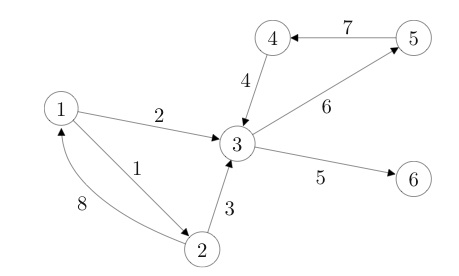
\includegraphics[height = 5 cm]{network-ex-incidence-mat.jpg}
\caption{An example of a network}
\label{efig:ex-network}
\end{figure}

\begin{figure}[h]
\centering

\includegraphics[height = 3 cm, width = 7cm]{ex-incidencematrix1.png}
\caption{The incidence matrix associated with Figure \eqref{efig:ex-network}}
\label{fig:incidence-matrix}
\end{figure}

The terms \(\|\sum_{c=1}^C\left(B_c^T \otimes I_n\right)\bar{x}_c\|^2\) and \( \eta^T\left(B_c^T \otimes I_n\right)\bar{x}_c \) of \eqref{aug-lagrange}, can be decomposed across edges, using the following lemma:

\begin{lemma}[Edge Decomposition]
\begin{equation}
\vectornorm{\sum_{c=1}^C\left(B_c^T \otimes I_n\right)\bar{x}_c}^2 = \sum_{j \in C_1}\left( D_j\vectornorm{x_j}_2^2 - \sum_{k \in N_j} x_j^Tx^k\right)
\end{equation}

and

\begin{equation}
\eta^T\sum_{c=1}^C\left(B_c^T \otimes I_n\right)\bar{x}_1 = \sum_{l\in C_c} \sum_{m\in N_l}sign\left(m-l\right)\eta_{ml}^T x_l
\end{equation}

where \(\eta\) is decomposed edge-wise: \(\eta = \left(\ldots, \eta_{ij},\ldots\right)\), such that \(\eta_{i,j} = \eta_{j,i}\), and is associated with the constraint \(x_i = x_j\).


\begin{proof}

\begin{align*}
u^Tu &= \sum	_{c_1=1}^C \sum	_{c_2=1}^C  \left(B_{c_1} \otimes x_{c_1}^T\right) \left(B_{c_2}^T \otimes x_c\right) \\
&= \sum_{c_1, c_2} B_{c_1}B_{c_2}^T \otimes x_{c_1}^Tx_{c_2}
\end{align*}

\(BB^T\) is a \(J \times J\) matrix, with the degree of the nodes on the main diagonal and \(-1\) in position \(\left(i,j\right)\) if nodes \(i\) and \(j\) are neighbours (i.e \(BB^T\) is the graph Laplacian). Hence, since we can write \(B_{c_1}B_{c_2}^T = w_{c_1}^TBB^Tw_{c_2}\), the trace of \(B_{c_1}B_{c_1}^T\) is simply the sum of the degrees of nodes with colour 1. 

For \(c_1 \neq c_2\),  \(B_{c_1}B_{c_2}^T\) corresponds to an off diagonal block of the graph Laplacian, and so counts how many neighbours each node with colour 1 has.

Finally, note that \(\eta \in \re^{nE}\) and can be written:

\begin{equation}
\eta = \sum_{c=1}^C w_c \otimes \eta_c
\end{equation}
where \(\eta_c\) is the vector of Lagrange multipliers associated across edges from colour \(c\). Now

\begin{align*}
\eta^Tu = \sum_{c_1=1}^C\sum_{c_2=1}^C w_{c_1}Bw_{c_2} \otimes \eta_{c_1}^Tx_c
\end{align*}
by the properties of Kronecker products, and the definition of \(B_c\). For \(c_1=c_2\), \(\eta^Tu\) is zero, as there are no edges between nodes of the same colour b definition. For \(c_1\neq c_2\), \(\eta^Tu\) counts the edges from \(c_1\) to \(c_2\), with the consideration that the edges from \(c_2\) to \(c_1\) are counted with opposite parity.
\end{proof}
\end{lemma}

Adding together this with the lemma, lets us write \eqref{aug-lagrange} as:

\begin{align}
L_\rho = \sum_{c=1}^C\sum_{j \in C_c} &\left( f\left(x_j\right) + \beta g\left(z_j\right)\right) + \nu^Tx_j \nonumber \\
& \text{        } \theta\left(x_j - z_j\right) + \frac{\rho}{2}D_i\vectornorm{x_j}^2 + \frac{\rho }{2}\|x_j-z_j\|^2
\label{generic-iterations}
\end{align}

where we have defined:

\begin{equation}
\nu_i = \left(\sum_{k \in \mathcal{N}_i} sign\left(k-i\right)\eta_{\{i,k\}} - \rho x_k \right)
\end{equation}

this is a rescaled version of the Lagrange multiplier, \(\eta\). 

Then by differentiating \eqref{generic-iterations} with respect to \(x_j\) and \(z_j\) we  can find closed forms for the updates as:

\begin{thm}
\begin{align}
x_j^{k+1} &:= \left(A_j^TA_j + (\rho D_J + 1) I\right)^{-1}\left(A_j^Ty_j +  z^k - \nu^{kT}\right)\\
z_j^{k+1} &:= S_{\beta/\rho}\left(x_j^{k+1} \right)
 \\
\theta_j^{k+1} &:= \theta_j^{k} + \rho \left(x^{k+1}-z^{k+1}\right) \\
\eta_j^{k+1} &:= \eta_j^k + \rho\left(\sum_{m \in N_j} z_m^k - z_j^k\right)
\label{dadmm_algo_lasso}
\end{align}
\end{thm}

This algorithm can be thought of as follows: each node performs an iteration of (non multi-block) ADMM - i.e. each node solves an approximate Gaussian least-squares problem and then soft-thresholds - and then exchanges the result of this computation with its one-hop neighbours. This explains the inclusion of an extra Lagrange multiplier: the multiplier \(\theta\) controls how far each node moves from its previous estimate in each iteration, whilst the multiplier \(\eta\) enforces consistency between nodes. Note that there is no communication of data between the nodes - only the result the computation in each round.

\subsection{DADMM-Lasso}

\subsection{DADMM-Dantzig-Selector}

\subsection{DADMM-MMV}
In this section we extend our results to the multiple measurement vector (\gls{mmv}) model of \cite{cotter2005sparse}. The model can be summarised as follows:

\begin{equation}
Y = AX + N
\end{equation}

Here, \(Y, N\in \re^{m\times p}\), \(x \in \re^{p\times n}\), \(A\in \re^{m \times n}\)

The \gls{mmv} model is an extension of \eqref{eq:system} where instead of a single sparse vector being estimated, a set of multiple (jointly) sparse vectors are recovered (under the assumption that these vectors share a common set of non-zeros).

The resulting optimisation problem is:

\begin{equation}
\argmin_X \vectornorm{X}_{2,1} \text{ s.t } Y=AX
\label{program:bpmmv}
\end{equation}

which can be recast in unconstrained form as:

\begin{equation}
\argmin_X \frac{1}{2}\vectornorm{AX-Y}_F^2 + \lambda\vectornorm{X}_{2,1}
\label{program:lassommv}
\end{equation}

This can be turned into a distributed optimisation problem, and so solved with \eqref{dadmm_algo_lasso}.

\section{Results} \label{sec:results}

The model described in section (\ref{sec:sensingmodel}), equation \eqref{system} was simulated, with a wideband signal of 201 channels and a network of 50 nodes (i.e. the signal will be sampled at a 1/4 of rate predicted by Nyquist theory). The mixing patterns were generated from iid Gaussian sources (i.e the matrix S had each entry drawn from an iid Gaussian source). Monte Carlo simulations were performed at SNR values ranging from 5 to 20, and the expected Mean Squared Error (MSE) of solutions of a centralised solver (spgl1) and a distributed solver (ADMM) were calculated over 10 simulations per SNR value. The results can be seen in fig (\ref{msevssnr1}). 

The MSE was calculated as follows:

\begin{equation}
\frac{\vectornorm{Z^k - Z*}}{\vectornorm{Z*}}
\end{equation}

where \(Z^k\) is the result of the algorithm at iteration \(k\), and \(Z^*\) is the optimal solution.

These results indicate that for both centralised and distributed solvers, adding noise to the system results in a degrading of performance. Interestingly note, that the distributed solver seems to (slightly) outperform the centralised solver at all SNRs. This is counter-intuitive, as it would be expected that centralised solvers knowing \textit{all} the available information would outperform distributed solutions. We conjecture that the updates described in section \eqref{sec:opt-on-graphs}, take into account differences in noise across the network. The distributed averaging steps, which form the new prior for each node, then penalise updates from relatively more noisy observations. This corroborates observations from \cite{bazerque2008}.

This observation is (partially) confirmed in figure (\ref{erroriterations}), which plots the progress of the centralised and distributed solvers (as a function of iterations) towards the optimum solution. The SNR is 0.5 (i.e the signal is twice as strong as the noise). Note that after around 300 iterations, the MSE of the distributed solver is consistently below that of the centralised solver.

\begin{figure}[h]
\centering
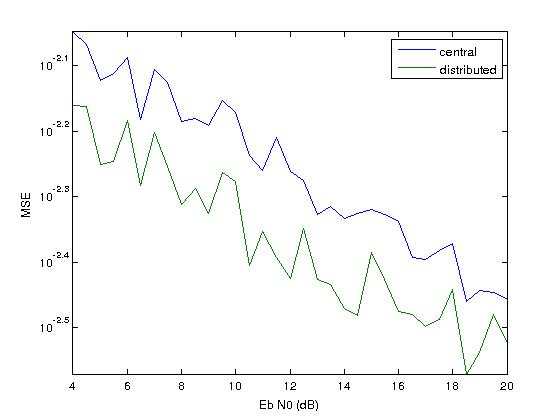
\includegraphics[height = 7.3 cm]{ebn0bbvsmse10ppnoH1logs.jpg}
\caption{Mse vs SNR for the sensing model, with AWGN only, showing the performance of distributed and centralised solvers}
\label{msevssnr0}
\end{figure}

\begin{figure}[h]
\centering
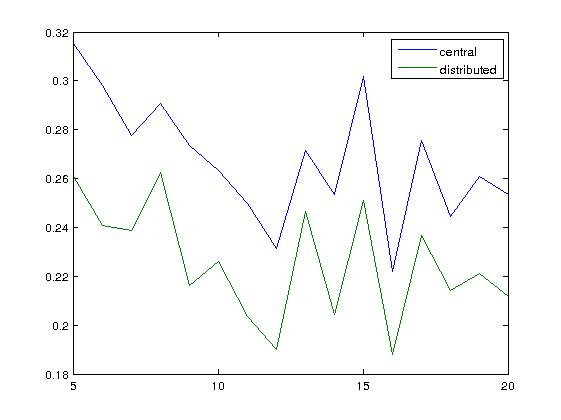
\includegraphics[height = 7.3 cm]{ebn0bbvsmse100ppwithH.jpg}
\caption{Mse vs SNR for the sensing model, showing the performance of distributed and centralised solvers}
\label{msevssnr1}
\end{figure}

\begin{figure}[h]
\centering
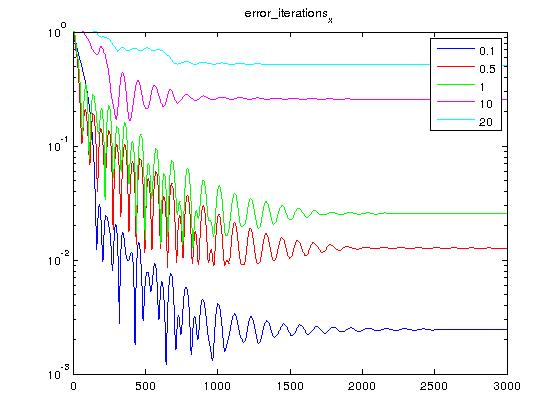
\includegraphics[height = 7.3 cm]{different_lambda.jpg}
\caption{The progress of the distributed solver as a function of the number of iterations, with different values of the regression parameter \(\lambda\)}
\label{fig:differentLambda}
\end{figure}

\begin{figure}[h]
\centering
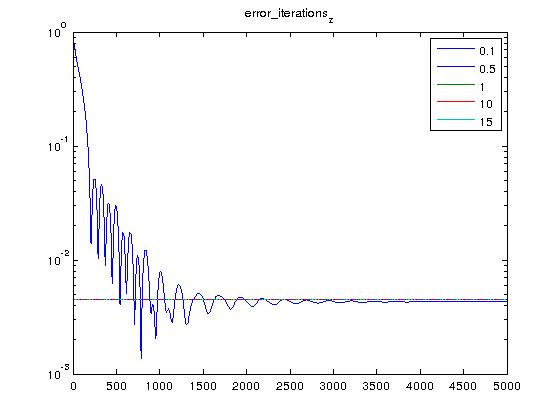
\includegraphics[height = 7.3 cm]{mse_iterations.jpg}
\caption{The progress of a distributed (blue) and a centralised (green) solver as a function of the number of iterations. The value of \(\lambda = 0.1\)}
\label{fig:erroriterations}
\end{figure}

\begin{figure}[h]
\centering
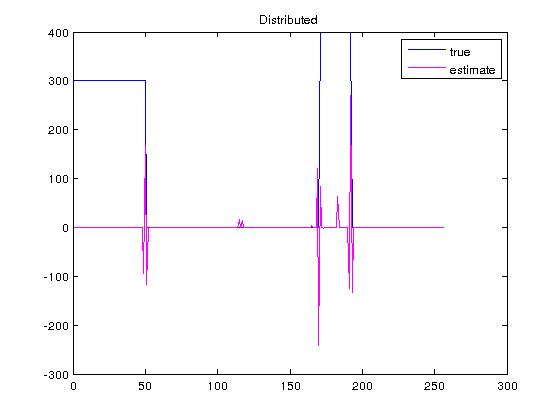
\includegraphics[height = 7.3 cm]{recon_spline.jpg}
\caption{The progress of a distributed (blue) and a centralised (green) solver as a function of the number of iterations. The value of \(\lambda = 0.1\)}
\label{fig:spline_recon}
\end{figure}

\begin{figure}[h]
\centering
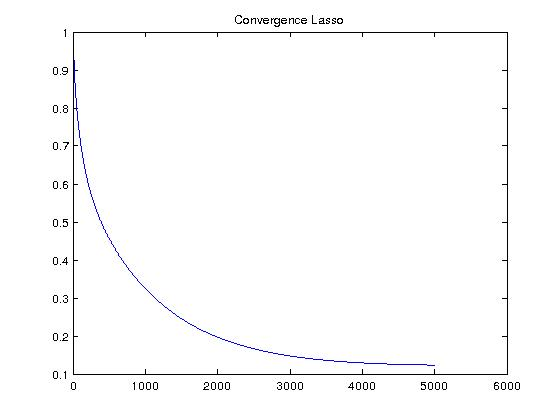
\includegraphics[height = 7.3 cm]{steps.jpg}
\caption{The progress of a distributed (blue) and a centralised (green) solver as a function of the number of iterations. The value of \(\lambda = 0.1\)}
\label{fig:steps_wavelets}
\end{figure}

\begin{figure}[h]
\centering
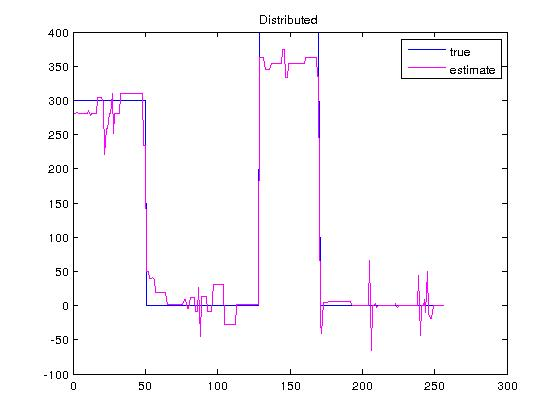
\includegraphics[height = 7.3 cm]{recon170815.jpg}
\caption{The progress of a distributed (blue) and a centralised (green) solver as a function of the number of iterations. The value of \(\lambda = 0.1\)}
\label{fig:wavelet_recon}
\end{figure}

\begin{figure}[h]
\centering
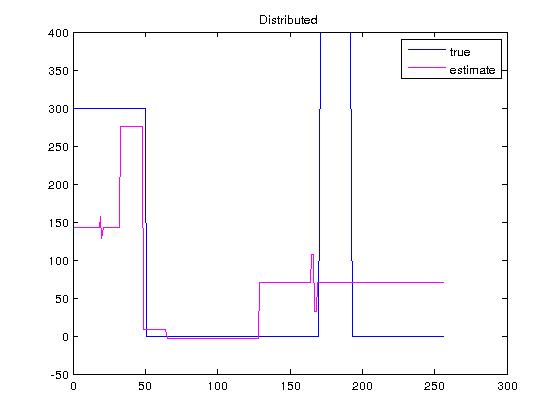
\includegraphics[height = 7.3 cm]{recon_new_bar.jpg}
\caption{The progress of a distributed (blue) and a centralised (green) solver as a function of the number of iterations. The value of \(\lambda = 0.1\)}
\label{fig:wavelet_recon_no_pwer_2}
\end{figure}

\begin{figure}[h]
\centering
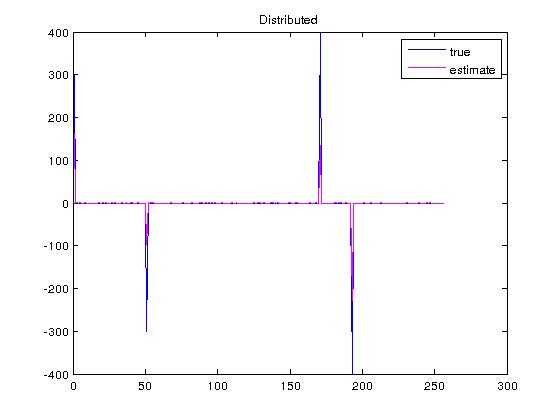
\includegraphics[height = 7.3 cm]{recon_difference.jpg}
\caption{The progress of a distributed (blue) and a centralised (green) solver as a function of the number of iterations. The value of \(\lambda = 0.1\)}
\label{fig:erroriterations}
\end{figure}

\begin{figure}[h]
\centering
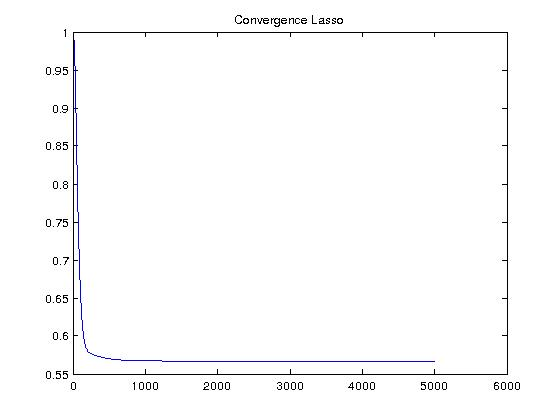
\includegraphics[height = 7.3 cm]{steps_difference.jpg}
\caption{The progress of a distributed (blue) and a centralised (green) solver as a function of the number of iterations. The value of \(\lambda = 0.1\)}
\label{fig:steps_difference}
\end{figure}

\begin{figure}[h]
\centering
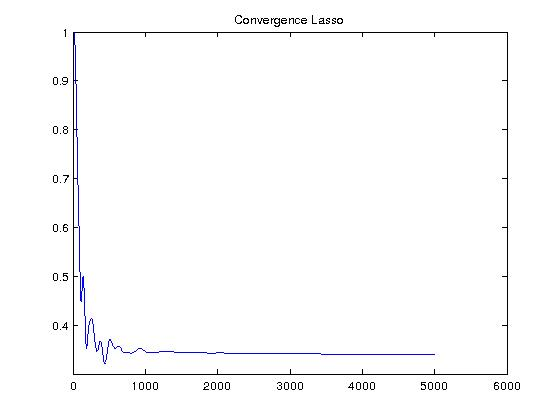
\includegraphics[height = 7.3 cm]{steps_splines.jpg}
\caption{The progress of a distributed (blue) and a centralised (green) solver as a function of the number of iterations. The value of \(\lambda = 0.1\)}
\label{fig:steps_splines}
\end{figure}

\begin{figure}[h]
\centering
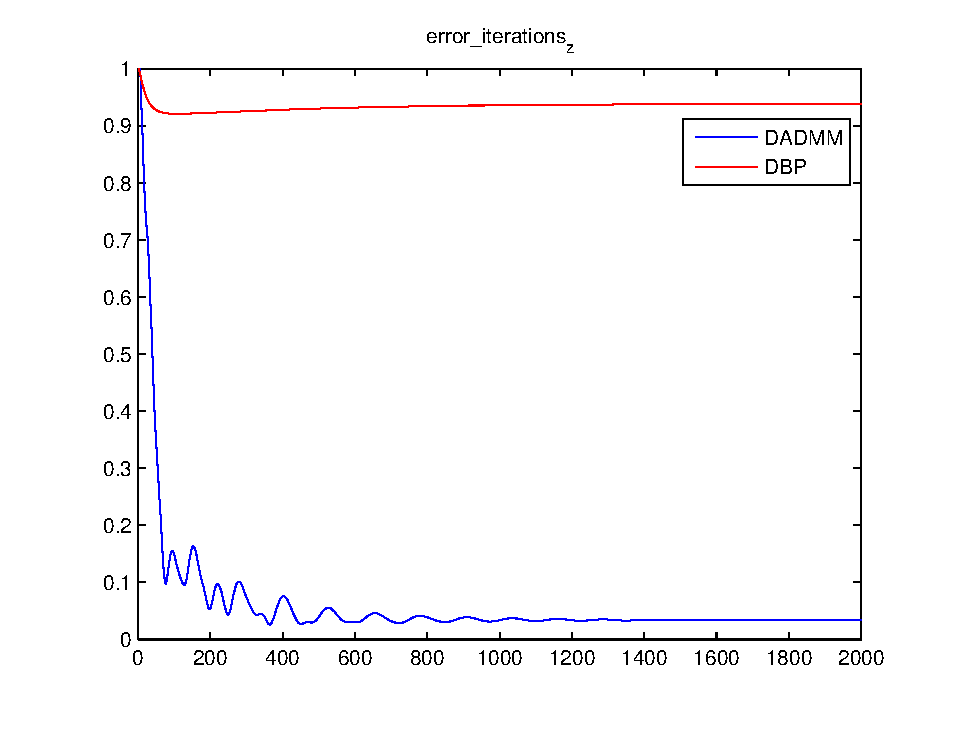
\includegraphics[height = 7.3 cm]{dadmmvsdbp.eps}
\caption{The progress of DADMM (blue) vs DBP (red) solvers as a function of the number of iterations. }
\label{fig:steps_splines}
\end{figure}

\begin{figure}[h]
\centering
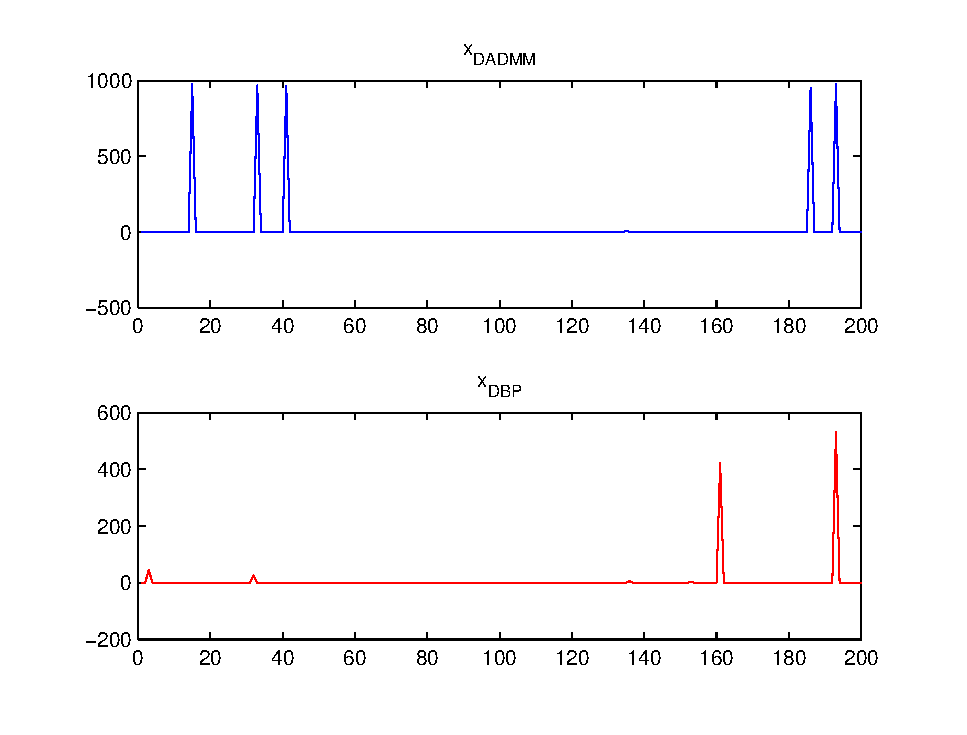
\includegraphics[height = 7.3 cm]{dadmmvsdbp_solutions.eps}
\caption{The solutions produced by DADMM and DBP}
\label{fig:steps_splines}
\end{figure}

\begin{figure}[h]
\centering
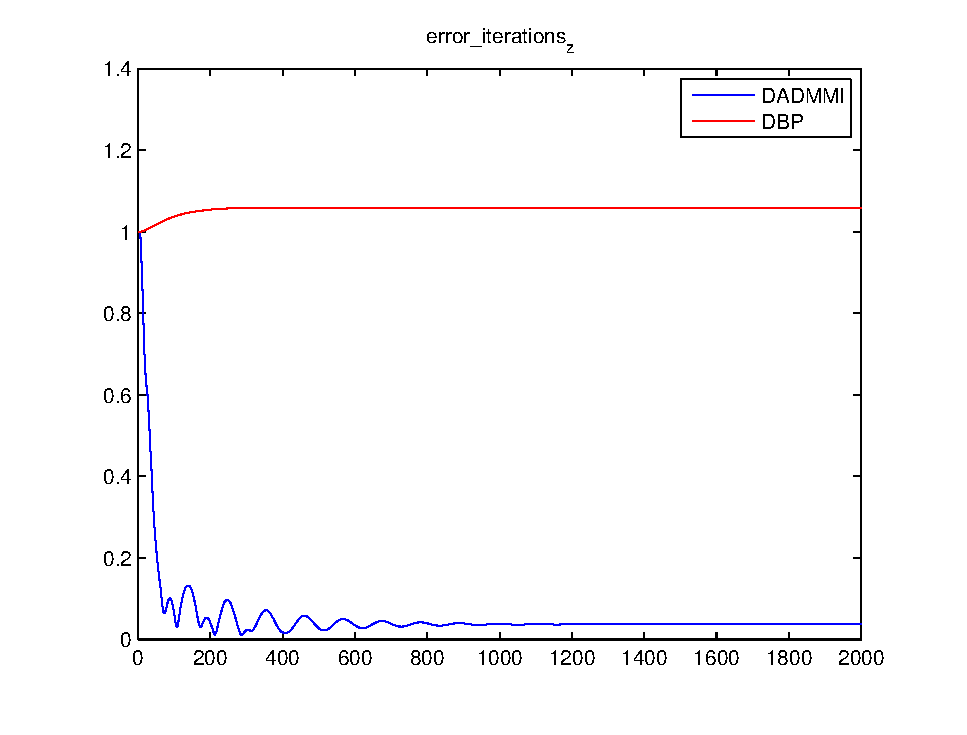
\includegraphics[height = 7.3 cm]{dadmmvsdbp_bad.eps}
\caption{The progress of a DADMM (blue) and DBP (red) }
\label{fig:steps_splines}
\end{figure}

\begin{figure}[h]
\centering
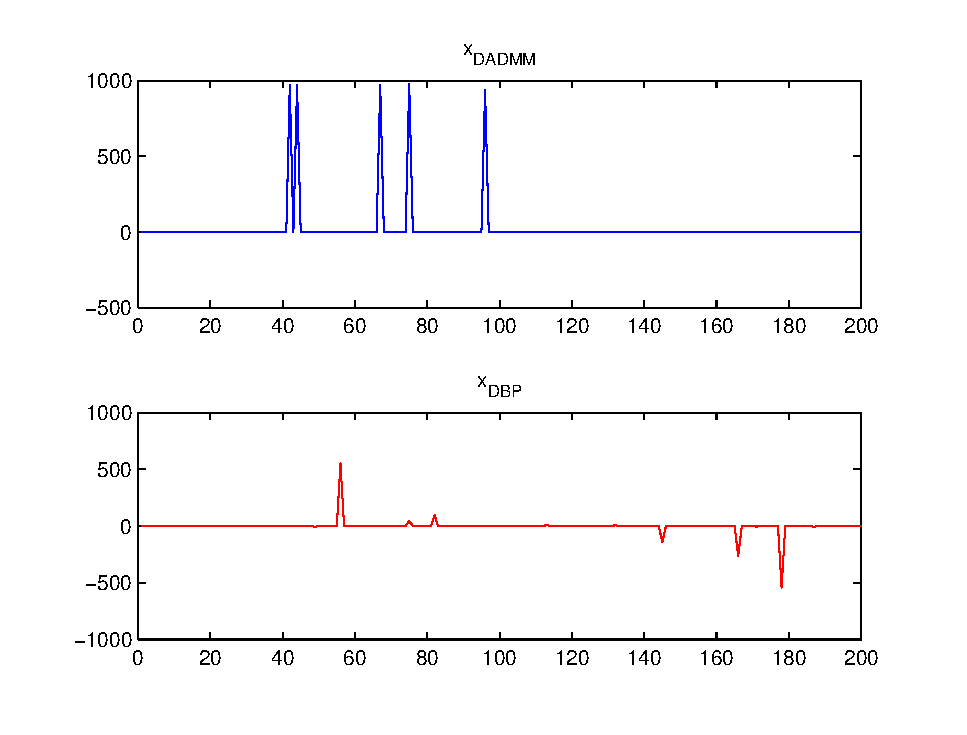
\includegraphics[height = 7.3 cm]{dadmmvsdbp_bad_solutions.eps}
\caption{The progress of a distributed (blue) and a centralised (green) solver as a function of the number of iterations. The value of \(\lambda = 0.1\)}
\label{fig:steps_splines}
\end{figure}

\begin{figure}[h]
\centering
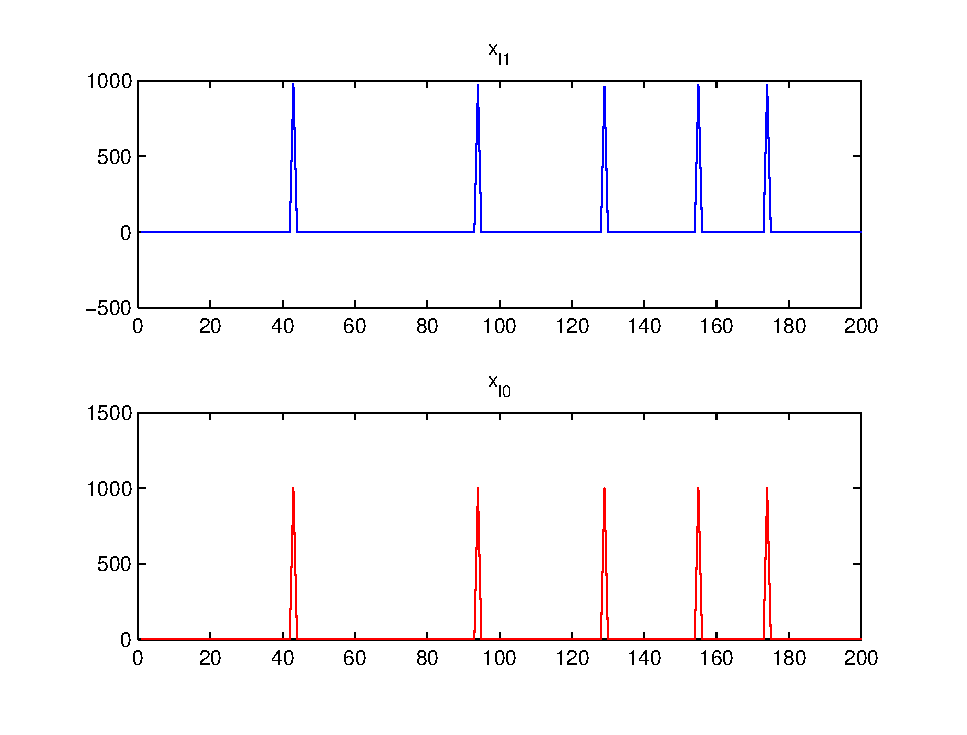
\includegraphics[height = 7.3 cm]{l1vsl0.eps}
\caption{The progress of a distributed (blue) and a centralised (green) solver as a function of the number of iterations. The value of \(\lambda = 0.1\)}
\label{fig:steps_splines}
\end{figure}

\begin{figure}[h]
\centering
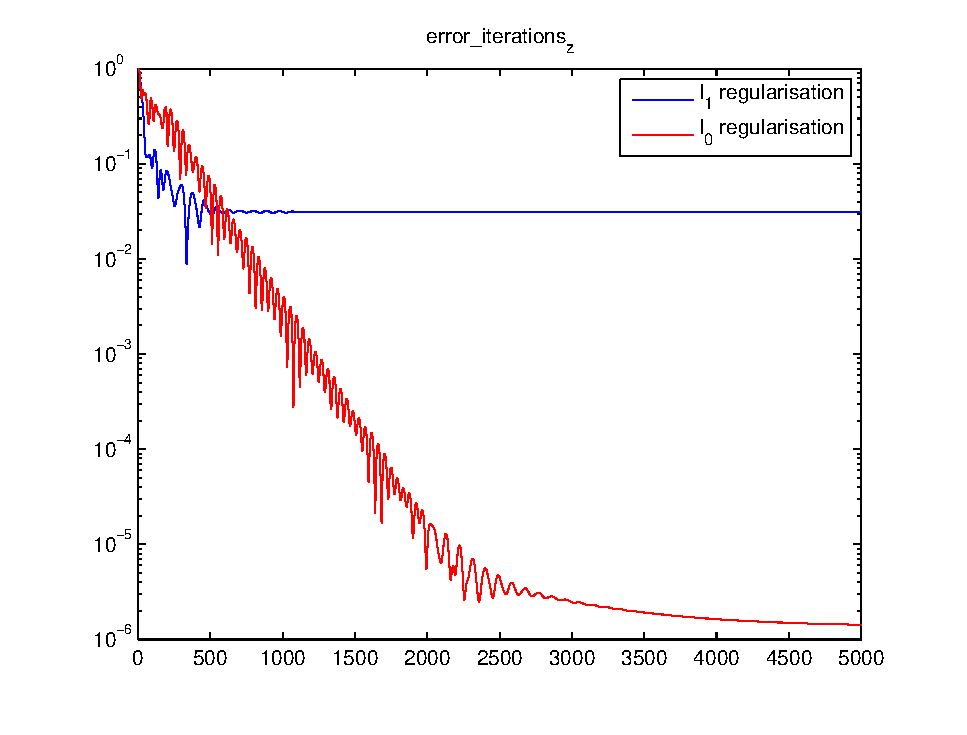
\includegraphics[height = 7.3 cm]{l1vsl0_iterations.eps}
\caption{The progress of a distributed (blue) and a centralised (green) solver as a function of the number of iterations. The value of \(\lambda = 0.1\)}
\label{fig:steps_splines}
\end{figure}


\section{Conclusions}
We have demonstrated an alternating direction algorithm for distributed optimisation with closed forms for the computation at each step, and discussed the statistical properties of the estimation. 

We have simulated the performance of this distributed algorithm for the distributed estimation of frequency spectra, in the presence of additive (white, Gaussian) and multiplicative (frequency flat) noise. We have shown that the algorithm is robust to a variety of SNRs and converges to the same solution as an equivalent centralised algorithm (in relative mean-squared-error).

We plan to work on larger, more detailed, models for the frequency spectra and to accelerate the convergence via Nesterov type methods to smooth the convergence of the distributed algorithm \cite{goldstein2014fast}. Specifically, we seek to dampen the ringing seen in Figure \ref{fig:erroriterations}

\chapter{Sensing with Heavyside Basis}
\section{Introduction}

In this chapter we develop a new model of frequency specra, amenable to distributed reconstruction. We then apply the alogorithm from chapter \ref{dist-opt}, combined with this model, to perform spectrum sensing.

Compressive sensing makes the assumption that the signal being sensed is sparse, however we cannot always guarantee that the frequency spectrum will always be sparse: for example, should TVWS become widely utilised, the spectra will not be sparse. However, even for highly occupied spectra, the gradient of the spectrum will be sparse. This has previously been exploited by \cite{tian2006wavelet}. 

Reconstructing the spectrum from compressive measurements could take place at a fusion centre, but such communications are expensive. It is more efficient therefore to design distributed algorithms where CRs communicate with their neighbours to reach consensus on the reconstruction, given each nodes' private data. However, regularising the reconstruction process would require global co-ordination if Total Variation (the \(l_1\) norm of the gradient of the signal) regularisation was chosen, as.

In this chapter we propose a different model for sensing the gradient of the frequency spectrum to \cite{tian2006wavelet} - a model which doesn't require Total Variation regularisation of the objective function. 

The structure of the chapter is as follows: in section \ref{sec:sig-model} we introduce the signal model, in \ref{sec:sensingmodel} we introduce the sensing model, and in section \ref{sec:results} we show some results of the reconstruction quality of this model. 

\section{Signal Model}\label{sec:sig-model}

Not all signals are sparse in an orthogonal basis: for example, many images are sparse in an over-complete dictionary (set of bases). In particular, frequency spectra for TVWS may no longer be sparse once opportunistic radios begin operating in these frequency bands. 

Instead we aim to reconstruct the gradient of the spectrum, as we assume that transitions are constant within a band. Consider the basis defined by the function:

\begin{equation}
l_i\left(x\right) =
\begin{cases}
1 & \text{if } x \leq i \\
0 & \text{ otherwise } 
\end{cases}
\label{basis}
\end{equation}

That is, \(l_i\) is a left-hand step function. 

The basis (\ref{basis}) can be expressed as a matrix in \(\re^{n \times n}\) as:

\begin{equation}
L = \begin{pmatrix}
 1 & 0 & 0 & 0  & 0 \ldots 0 \\
  1 & 1 & 0 & 0  & 0 \ldots 0\\
     1 & 1 & 1 & 0  & 0 \ldots0  \\
    \ldots  \\
     1 & 1 & 1 & 1  & 1 \ldots 1 
\end{pmatrix}
\end{equation}

By direct computation, this inverse of \(L\) is:

\begin{equation}
D = \begin{pmatrix}
 1 & 0 & 0 & 0  & 0 \ldots 0 \\
  -1 & 1 & 0 & 0  & 0 \ldots 0\\
     0 & -1 & 0 & 0  & 0 \ldots0  \\
    \ldots  \\
     0 & 0 & 0 & 0  \ldots -1 & 1
\end{pmatrix}
\end{equation}

We model our PSD signal \(g\) as a linear combination of the basis functions (\ref{basis}):

\begin{equation}
g\left(x\right) = \sum_i a_i l_i\left(x\right) = L^Ta
\label{basis-expansion}
\end{equation}

where \(a = (a_1, \ldots, a_n\) are the coefficients in this basis expansion, and \(l_i\) are the rows of \(L\). Note that as defined, \(g\) is a column vector.

\begin{proposition}
\begin{equation}
D^Tg = a
\end{equation}
\label{def:a}
\end{proposition}
\begin{proof}

\begin{align}
D^Tg &= D^T L^T a \\
&= \left(LD\right)^Ta \\
&= a
\end{align}

as \(LD = I\).

\end{proof}

\section{Sensing Model}\label{sec:sensingmodel}

We consider a radio environment with a single primary user (PU) and a network of \(J\) nodes collaboratively trying to sense and reconstruct the PU signal in a fully distributed manner by local communication and regularisation only.

We try to sense and reconstruct a wideband signal, using a network of \(J\) (= 50) nodes placed uniformly at random within the square \(  \left[0,1\right]\times \left[0,1\right] \). 

We consider the frequency domain measurements, formed by each node mixing the signal with a random Gaussian signal \(A_j \in \re^n\). The measurements taken at node \(j\) are:

\begin{equation}
y_j = A_jH_jg + w_j
\label{dist_system}
\end{equation}

where \(H_j \in \re\) is the scalar channel gain, and \(w_j \sim \mathcal{N}(0,\sigma^2_n) \in \re \) is additive white Gaussian noise. 

For the purposes of comparison in section (\ref{sec:results}), this corresponds to the concatenated system:

\begin{equation}
y = AHg + w
\label{system}
\end{equation}

where \(H \in \re^{n \times n}\) is a block diagonal matrix of channel gains.

The system  \ref{system} can then be solved (in the sense of finding the sparse vector \(a\) (\ref{basis}) by convex optimisation via minimising the objective function:

\begin{equation}
\hat{a} = \argmin_{a} \frac{1}{2}\|AHL^{T}a-y\|_2^2 + \lambda \|a\|_1
\label{opt}
\end{equation}

where \(\lambda\) is a parameter chosen to promote sparsity. Larger \(\lambda\) means sparser \(a\).

\section{Results} \label{sec:results}

The model described in section \eqref{sec:sensingmodel}, equation \eqref{system} was simulated. The signal \(g \in \re^{300} \) was composed of 3 rectangular pulses, mimicking primary user signals in TVWS, as shown in figure \eqref{different_sigs} (a). The signal was put through a Rayleigh channel, before being sensed by the nodes. The network was generated as a random geometric graph in \([0,1] \times [0,1]\), with 50 nodes. If the network wasn't connected, it was redrawn. 200 mixing patters were drawn i.i.d from a \(\mathcal{N}\left(0, \sigma^2 I_{300} \right) \) distribution, with \(\sigma^2 = 1/200\), to from the matrix \(A\in  \re^{200 \times 300}\).

Monte Carlo simulations were performed at 18 \(\sigma^2_n\) values ranging from 1 to 10 and the expected Mean Squared Error (MSE) of solutions of a centralised ADMM solver and a our distributed solver \ref{sec:algo-lasso} were calculated over 500 repetitions with 1200 iterations (\(k\)) per repetition.

The MSE was calculated as follows:

\begin{equation}
\frac{\vectornorm{L^tz^k - g^*}}{\vectornorm{g^*}}
\end{equation}

where \(z^k\) is the result of the algorithm at iteration \(k\), and \(g^*\) is the optimal solution.

The SNR for each repetition was calculated as

\begin{equation}
\frac{\vectornorm{g^*}}{\vectornorm{w}}
\end{equation}

and averaged over the 500 repetitions. The results are shown in figure \eqref{msevssnr0}. Following \cite{Chen1998}, for each repetition we chose 

\begin{equation}
\lambda = \sqrt{2\sigma^2_n\log{n}}
\end{equation}

The error bars indicate the empirical variance across the 500 repetitions.

These results indicate that for both the centralised and distributed solvers, their performance degrades as the noise power increases in a roughly log-linear fashion. The performance of the distributed algorithm is consistently worse than the centralised version, this contrasts with results from \cite{bazerque2008}; this is due to the differing sparsity models: \cite{bazerque2008} use a joint space and frequency model for the sparsity, and as such observe an spatial averaging out of noise when using a distributed solver. The performance of DADMM is within the error bars of the centralised version at low SNR, and gap in performance between the two versions is no more than \(10^{-2}\). Even at relatively lower SNRs both solvers reach a solution within \(10^{-1}\) of the optimal (as measured by normalised MSE), which will be adequate for the task of spectrum sensing. For example the reconstructions in figures \eqref{different_sigs} (c) and (d) show realisations of the reconstruction from DADMM with \(\sigma^2_n = 5\) and \(\sigma^2_n = 20\) respectively. It is still possible to distinguish the occupied bands from unoccupied frequencies for both reconstructions.

The distributed algorithm has consistently larger variance, than the centralised solver at all SNRs. This is due to individual nodes only having access to a subset of the data to perform calculations on: the variance will be proportional to the square-root of number of data samples at each node, which are fewer than the total number of samples available to the centralised solver. 

In figure \eqref{fig:differentLambda}, we plot the progress of DADMM along the solution path for a variety of regularisation parameters \(\lambda\). The y-axis is the relative (unormalised) MSE between the optimal solution and the current iteration, and the x-axis is the iteration number. We note that for a fixed \(\lambda\) there is a single unique optimal solution, which DADMM converges to (in the sense of stationary error between consecutive iterations). This solution may not be attained in the allotted number of iterations, as the rate of convergence is determined by \(\lambda\), \(\rho\) and the eigenvalues of the Laplacian of \(G\). The paper \cite{shi2014linear}, proves linear convergence for DADMM, with explicit expressions for the rate. In particular the rate convergence of DADMM is affected by the choice of \(\lambda\): smaller \(\lambda\) corresponds to slower convergence - this is intuitive as solutions with fewer non-zero components should require fewer iterations to fully specify. Notice that for some \(\lambda\)s the solution path exhibits phenomenological  behaviour similar to damped oscillations: this phenomena has been explored in \cite{nishihara2015general} and \cite{su2014differential}.  

\begin{figure}[h]
\centering
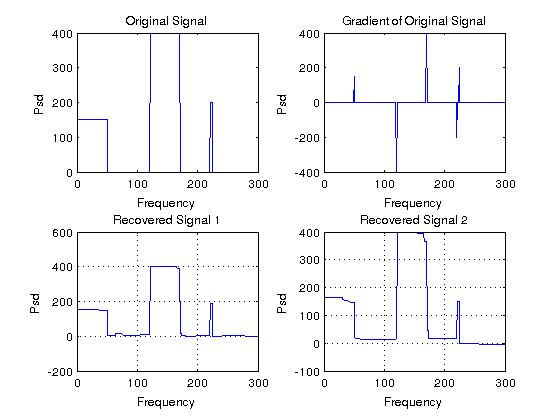
\includegraphics[height = 7.3 cm]{signal_and_recovery.jpg}
\caption{Left to right: (a) The original signal. (b) The gradient \eqref{def:a} of the original signal. (c) Recovery using DADMM, 1000 iterations, \(\sigma^2_n = 5\). (d) Recovery using DADMM, 1000 iterations, \(\sigma^2_n = 20\)  }
\label{different_sigs}
\end{figure}

\begin{figure}[h]
\centering
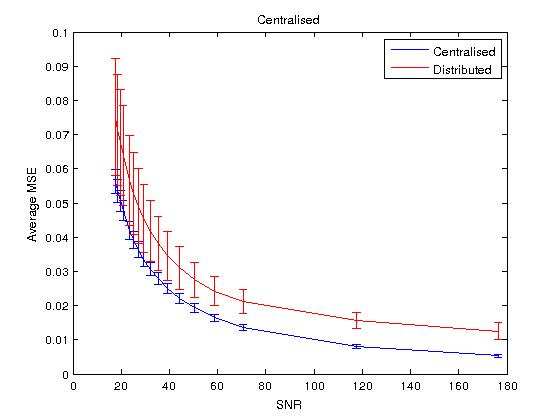
\includegraphics[height = 7.3 cm]{Cent_Vs_Distrib_snr.jpg}
\caption{MSE vs SNR for the sensing model showing the performance of distributed and centralised solvers. The performance of DADMM is consistently within \(10^{-2}\) of ADMM, and within the error bars of ADMM at low SNRs. The variance of estimates produced by DADMM is larger than ADMM, due to nodes performing computations on a subset of data. Both estimates are consistently within \(10^{-1}\) of the optimal solution, which is sufficient to classify occupied bands.} 
\label{msevssnr0}
\end{figure}

\begin{figure}[h]
\centering
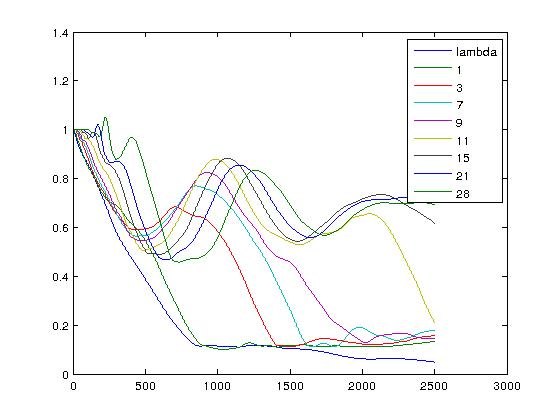
\includegraphics[height = 7.3 cm]{continuations_errors.jpg}
\caption{The progress of the distributed solver as a function of the number of iterations, with different values of the regression parameter \( \lambda \). For a fixed \( \lambda \) there is a single unique optimal solution, with higher \( \lambda \) favouring sparser solutions. The convergence of DADMM is slowed by smaller \( \lambda \). This is intuitive: solutions with fewer non-zero components should be identified in fewer iterations.}
\label{fig:differentLambda}
\end{figure}

\section{Conclusions}
We have simulated the performance of this distributed algorithm for the distributed estimation of frequency spectra, in the presence of additive (white, Gaussian) and multiplicative noise. We have shown that the algorithm is robust to a variety of SNRs and converges to a similar solution as an equivalent centralised algorithm (in relative mean-squared-error).

\chapter{Compressive Inference}
\section{Introduction}

The bulk of research into Compressive Sensing has been on designing efficient matrices to capture the signal, and on creating fast algorithms for the sample inversion. However, reconstructing a signal is not the only interesting signal processing task: there is also filtering, signal classification and inference based upon the signal. In this chapter, we investigate a method of applying ideas from Compressive Sensing to determine the occupancy of a spectral band, without ever reconstructing the singal from the samples as an intermediate step.

The purpose of the excercise is to drastically reduce the number of samples required to make a descsion about whether a band is occupied - for sensing matrices satisfying the RIP, the number of samples required to infer properties about the signal is considerably smaller than the number of samples required to reconstruct the signal. 

This chapter outlines the basic theory behind compressive inference, with some worked examples - estimating a single spike from compressed data, estimating a single rectangle from compressed data, and estimating synthetic frequency spectra from data. 

We begin by quickly review the RIP (definition \eqref{def:RIP}) and its extension to stable embeddings, and how these ideas make it possible to infer properties about signals without reconstruction as intermediate step. We then define a maximum likelihood estimator to identify sparse components of a signal.

We then extend these ideas to the problem of maximum likelihood compressed estimation of a signal in some known set of basis functions. Finally, we apply these ideas to classification of a sequence of frequency bands. To our knowledge, this is the first time these techniques have been used to directly estimate spectral occupancy.

We demonstrate the efficiacy of our methods by computing ROC curves for noisy signals, at varying levels fo undersampling (from 5\% to 100\%) and at various levels of noise power.

\section{Theory}

The work of Candes and Tao \cite{Candes2006} and Donoho \cite{Donoho2006} has established that many real-world signals can be effectively captured via a small number of random projections relative to the dimension of the signal. For example, a 5 megapixel image can be thought of as a vector in \(\re^{5,000,000}\). However, it is well known that images have relatively few wavelet coefficients; this is exploited by the JPEG-2000 standard, which can represent the image as a 64-kb file (i.e a point in \(\re^{64,000}\).

Classically, for perfect signal reconstruction, we must sample a signal such that the sampling rate must be at least twice the maximum frequency in the bandlimited signal. The continuous time signal can then be recovered using an appropriate reconstruction filter (e.g. a sinc filter). See Chapter \ref{chap:nyq}, section \ref{sec:classic-sensing} for more detail.

In contrast Compressive Sampling suggests that by adding randomness into the measurement process, a sparse (or compressible signal) may be accurately sensed with far fewer measurements:

\begin{equation}
y = Ax + w
\end{equation}


where \(A \in \mathbb{R}^{m \times n}\) is a matrix with random entries, \(x \in \mathbb{R}^n\) is the signal we capture, \(y \in \mathbb{R}^m\) is the result of the measurement process and \(w \sim N\left(0,1\right) \in \mathbb{R}^m\) is additive white Gaussian noise, \(m < n\).

Some technical conditions on the matrix \(A\) have to satisfied for it: namely the transformation defined by \(A\) must behave like an approximate Isometry, and it must be incoherent. We recap definitions from Chapter \ref{chap:cs} for expository convenience.

\begin{definition}[RIP]
We say that a matrix \(A\) satisifes the RIP of order \(\delta\) if \(\exists\) a \(\delta \in \left(0, 1\right)\) such that:
\begin{equation}
\left(1 - \delta\right) \vectornorm{x}_2^2 \leq \vectornorm{Ax}_2^2 \leq \left(1 + \delta\right) \vectornorm{x}_2^2
\end{equation}
i.e. \(A\) approximately preserves the lengths of all \(s\)-sparse vectors in \(\re^n\). 
\end{definition}

\begin{definition}[Coherence]
The mutual coherence of a matrix \(A\) is the absolute normalised inner product between different columns from \(A\). Denoting the \(k\)-th column in \(A\) by \(a_k\), the mutual coherence is given by:
\begin{equation}
\mu(A) = \max_{1\leq i,j\leq n , i\neq j} \frac{|\langle a^T_i, a_j\rangle|}{\vectornorm{a_i}_2\vectornorm{a_j}_2}
\end{equation}
\end{definition}

This implies that sensing with incoherent systems is good, and efficient mechanisms ought to acquire correlations with random waveforms (e.g. white noise).

\textbf{Theorem} \cite{Candes2006}
Fix x \(\in \mathbb{R}^n\) with a sparse coefficient basis, \(x_{i}\) in \(\psi\). Then a reconstruction from \(m\) random measurements is possible with probability \(1 - \delta\) if: 

\begin{equation}
m \geq C \mu^2(A) S \log\left(\frac{n}{\delta}\right)
\end{equation}
\label{minsamples}

where \( \mu(A)\) is the coherence of the two bases, and \(S\) is the number of non-zero entries on the support of the signal. 

In this new sensing paradigm, the complexity is shifted to the reconstruction process, where with high probability Donoho proved \cite{donoho2004neighborly}, that the minimiser of the program:

\begin{equation}
\argmin_{x} \frac{1}{2}\vectornorm{y-Ax}_2^2 + \lambda\vectornorm{x}_1
\end{equation}

coincides with the sparsest solution to the under-determined system of linear equations. Thus we are able to sense sparse signals with random waveforms, and reconstruct them via linear programming.

However, signal reconstruction is not the only interesting signal processing task. Filtering, classification, detection, and estimation are also required in real world systems. For these tasks it was thought that signal reconstruction must be performed first, and then classical signal processing techniques could be brought to bear on the reconstruction. 

There is some tension in this idea however: since the measurement matrix is an approximate isometry, some (as yet unspecified) operations on the measurements \(y\) should correspond to inference tasks (such as filtering and estimation) on \(x\). This means that performing inference needn’t require the reconstruction of the signal. 

The papers \cite{davenport2010signal} and \cite{davenport2007smashed} provide an introductory answer for the cases of filtering, detection, classification and estimation.

There has been a little work applying this line of work: \cite{schnelle2012compressive} shows how to design a Phase-Locked loop directly in the compressive domain and applies it to demodulating FM signals, and \cite{davenport2010wideband} extends this idea to a wideband compressive radio receiver. Matched filtering from compressive samples is performed in \cite{eftekhari2013matched}, and 

The structure of this document is as follows: sections \eqref{sec:prelims}, is a literature review of relevant material from compressed sensing, Wishart matrices, and maximum likelihood estimation of uncompressed signals in noise. Section \eqref{sec:estimation} gives an overview of the problem of estimating a signal from a known set of basis functions. 

\section{Compressive Estimation} \label{sec:estimation}
In this section, we develop some intuition into constructing estimators for the signal \(s\) directly on the compressive measurements:

\begin{equation}
y = As + n
\end{equation}
\\
where \(A \in \re^{m \times n} \), \(A_{ij} \sim \mathcal{N}\left(0,1/m\right)\), and \(n \in \re^n\) is AWGN. We again assume that \(s\) comes from a fixed set of models, parametrised by some set \(\Theta\). 

The likelihood for this model is, (as y is a normal random variable):

\begin{equation}
f\left(y \mid s\right) = \left(\frac{1}{\sqrt{2\pi}} \right)^m \exp{\left( - \frac{\left(y-As\right)^T  \left(y-As\right)}{2} \right)}
\end{equation}

Taking the logarithm and expanding, we find

\begin{equation}
\ln{f} = -y^Ty - s^TA^TAs + 2\langle y, As \rangle
\end{equation}

which is equal to:

\begin{equation}
ln{f} = - \vectornorm{y}_2^2 - \vectornorm{As}_2^2 + 2\langle y, As \rangle
\label{log-like}
\end{equation}
The first term of \eqref{log-like} is constant, for the same reasons as in section \eqref{sec:estimation}. The term 

\begin{equation}
\vectornorm{As}^2_2 = \langle As, As\rangle
\end{equation}

can be written as 

\begin{equation}
\langle A^T As, s\rangle
\end{equation}

We will replace this with its expectation \(\ep{\left( \langle A^T As, s\rangle \right)}\)

\begin{align*}
\ep{\left(\langle A^T As, s\rangle\right)} &=  \ep{\sum_{i=1}^n (A^TAs)^T_i s_i} \\
&= \sum_{i=1}^n \ep{(A^TAs)_i s_i} \\
&= \sum_{i=1}^n (\frac{1}{m}e_i s_i)^T_i s_i \\
&= \frac{1}{m} \langle s, s \rangle
\end{align*}

because

\begin{equation}
\ep{A^TA} = \frac{1}{m}I
\end{equation}

as it is a Wishart matrix (see section \ref{sec:wishart}, theorem \eqref{thm:wishart-mean}). 
\\
So we can further approximate \eqref{log-like}:

\begin{equation}
\ln{f} = - \vectornorm{y}_2^2 + \frac{1}{m}\vectornorm{s}_2^2 + 2\langle y, As \rangle
\label{approx-log-like}
\end{equation}

The only, non-constant part of \eqref{approx-log-like} is the third term and so we define the estimator:

\begin{equation}
\hat{s} = \argmax_{\Theta} \langle y , As\left(\Theta\right)\rangle
\label{eq: compressive-estimator}
\end{equation}

For the case where \(s\) can be expanded in an orthonormal basis \(s = \sum_{i=1}^n \alpha_i\phi_i\), the maximum likelihood estimator is:

\begin{equation}
\hat{s} = \sum_{i=1}^n m\langle y, A\phi_i\rangle \phi_i
\end{equation}
\\
\\
Consider the case where \( y = As\) (no noise). Then

\begin{align*}
y^TA\phi_j &= \sum_i \alpha_i \phi_i^TA^TA\phi_j
\end{align*}

So 

\begin{align*}
y^TA\phi_j &= \sum_i \alpha_i \phi_i^TA^TA\phi_j \sim \frac{\alpha_i}{m} \delta_{ij}
\end{align*}

giving
 
\begin{equation}
\hat{\alpha_i} = m\left(y^TA\phi_j\right)
\end{equation}

\begin{remark}
The matrix \(M = A^TA\) is the projection onto the row-space of \(A\). It follows that \(\vectornorm{Ms}_2^2\) is simply the norm of the component of \(s\) which lies in the row-space of \(A\). This quantity is at most \(\vectornorm{s}_2^2\), but can also be \(0\) if \(s\) lies in the null space of \(A\). However, because \(A\) is random, we can expect that \(\vectornorm{Ms}_2^2\) will concentrate around \(\sqrt{m/n}\vectornorm{s}_2^2\) (this follows from the concentration property of sub-Gaussian random variables \eqref{cond:sub-Gauss concetration}).
\end{remark}

\subsection{Example: Single Spike}
We illustrate these ideas with a simple example: estimate which of \(n\) frequencies \(s\) is composed of.

A signal \(s \in \re^{300}\) composed of a single (random) delta function, with coefficients drawn from a Normal distribution (with mean 100, and variance 1) i.e 

\begin{equation}
s = \alpha_i \delta_i
\end{equation}
\\
with 

\begin{equation}
a_i \sim \mathcal{N}\left(100, 1\right)
\end{equation}

and the index \(i\) chosen uniformly at random from \([1, n]\).
\\
The signal was measured via a random Gaussian matrix \(A \in \re^{100 \times 300}\), with variance \(\sigma^2 = 1/
100 \) and the inner product between \(y = As\) and all 300 delta functions projected onto \(\re^{100}\) was calculated:

\begin{equation}
\hat{\alpha}_j = m\langle (A\alpha_i\delta_i), A\delta_j \rangle
\end{equation} 

We plot the \(\hat{\alpha_j}\) below, figure \ref{fig:new_basis_25}, (red circles), with the original signal (in blue, continuous line). Note how the maximum of the \(\hat{\alpha_j}\), coincides with the true signal.

\begin{figure}[h]
\centering
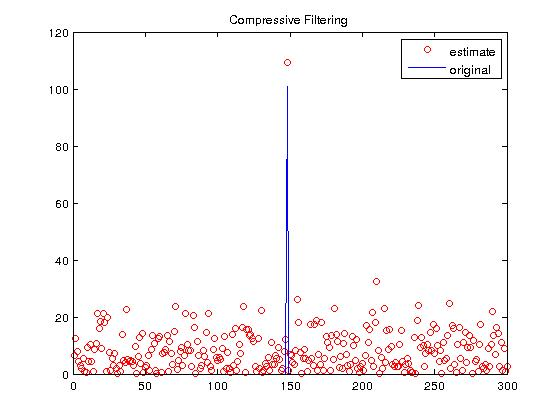
\includegraphics[height = 7.3 cm]{1spike_legend.jpg}
\caption{}
\label{fig:new_basis_25}
\end{figure}

\subsection{Estimating a single rectangle}

We show how to estimate the signal, composed of a single rectangle \eqref{fig:rectangle} expanded in the following basis

\begin{figure}[h]
\centering
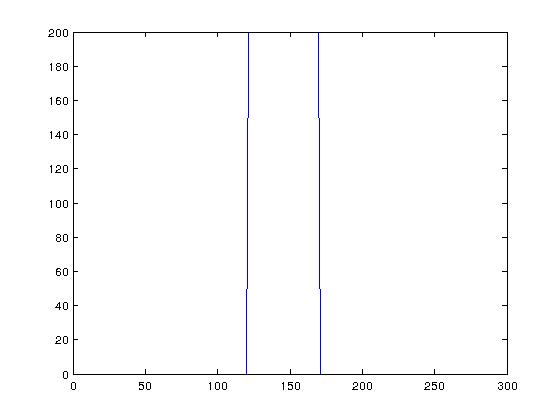
\includegraphics[height = 7.3 cm]{g.jpg}
\caption{}
\label{fig:rectangle}
\end{figure}

\begin{equation}
f_i\left(x\right) =
\begin{cases}
1 & \text{if } x \leq i \\
0 & \text{ otherwise } 
\end{cases}
\label{basis}
\end{equation}

We model our signal \(g\) as a linear combination of the basis functions (\ref{basis}):

\begin{equation}
g\left(x\right) = \sum_i a_i f_i 
\label{basis-expansion}
\end{equation}

To find the \(a_i\), we correlate (take the inner product of) the signal against the basis (\ref{basis}).

\begin{definition}
\begin{align}
h_j &= \langle g, f_j \rangle \\
&= \sum_j g\left(x\right) f_j\left(x\right) \\
&= \sum_j a_i f_i\left(x\right) f_j\left(x\right) \\
&= a_i \langle f_i, f_j\rangle \\
&\left(= \sum_{x=1}^j g\left(x\right)\right)
\end{align}
\end{definition}

As per the previous sections, we take compressive measurements:
\begin{equation}
y = Ag
\end{equation}
\\
where \(A \in \re^{m \times n} \), \(A_{ij} \sim \mathcal{N}\left(0,1/m\right)\), and then compute 
\begin{equation}
\langle y, Af_i\rangle = a_j  f_j^TA^tAf_j \sim \frac{a_j}{m} \langle f_j, f_i \rangle
\end{equation}
for the set of basis vectors \(f_1 \ldots f_n\) i.e. the estimator from the previous section, corresponding to this set of basis functions \eqref{eq: compressive-estimator}. 

We then form the vector 

\begin{equation}
\hat{h} = m \sum_i \langle y, Af_i\rangle f_j \sim h
\label{ss-estimator}
\end{equation}

An example can be seen in figure \ref{fig:hhat}, for a matrix \(A \in \re^{200 \times 300}.\)

\begin{figure}[h]
\centering
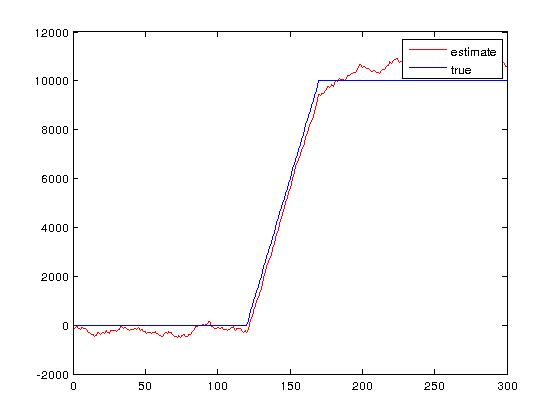
\includegraphics[height = 7.3 cm]{hhat.jpg}
\caption{}
\label{fig:hhat}
\end{figure}

\subsection{Estimating Frequency spectra}

Continuing from the previous (sub)-section we can create an estimate of \(g\), by the following procedure:

\begin{itemize}
\item Estimate the coefficients of the basis \(\hat{a}\) using \(\hat{a} = F^{-1} \hat{h}\)
\item Choose the \(k\) largest (for some \(k\) to be determined later).
\item Between the indices of the \(k\) \(\hat{a}\) take the average of the signal \(L^{-1}\hat{h}\).
\end{itemize}


\begin{figure}[h]
\centering
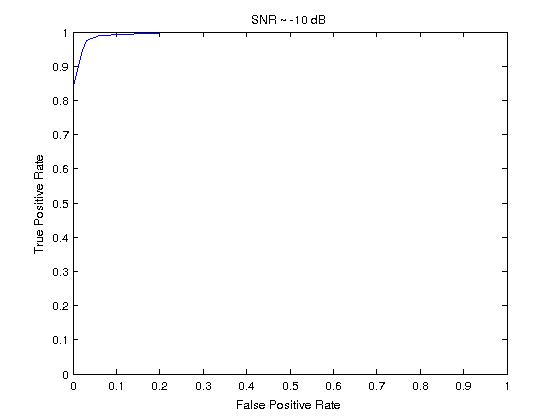
\includegraphics[height = 7.3 cm]{roc_minus_10.jpg}
\caption{ROC for synthetic data, midly noisy}
\label{fig:hvb}
\end{figure}

\begin{figure}[h]
\centering
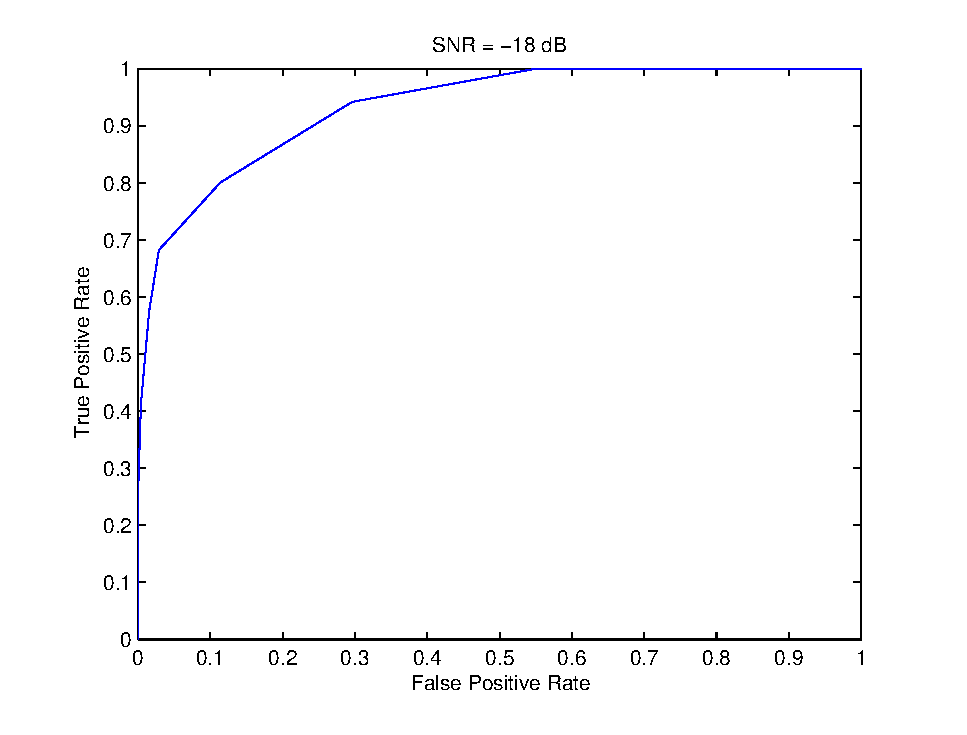
\includegraphics[height = 7.3 cm]{roc_minus_18.eps}
\caption{ROC for synthetic data, very noisy}
\label{fig:hvb}
\end{figure}

\chapter{Results on OFCOM Data}
\section{Introduction}

This chapter applies the methods of chapters \ref{chap:dist-opt} and \ref{chap:rect-basis}, specifically algorithms \ref{dadmm_algo_lasso}, \ref{alg:single-slot} and \ref{alg:multiple-shot} to a data set of TVWS measurements captured by OFCOM in the band 440-780MHz. The OFCOM dataset was taken in Southwark, UK during May 2014.

This chapter is organised as follows: we first describe the dataset in detail, and show example PSD captures for it, then we show results of the distributed estimation algorithm (presented in chapter \eqref{chap:dist-opt}), with estimation in the Heavyside basis. This algorithm is performed over a network of nodes, and reconstructs the sensed PSD via an iterative denoising procedure derived from the LASSO functional. It should be noted that this is the largest experiment of its kind: previous work has featured experimental results on far smaller datasets, or featured algorithms whos steps took considerably longer to reach an acceptable solution. We compare results produced by our algorithm to results from copetative algorithms, and discuss the relative performance in terms of reconstruction quality, classification accuracy and algorithm speed. 

We then present results of the techineques outlined in chapter \eqref{chap:cs-inference}, specifically algorithms \ref{alg:single-slot} and \ref{alg:multiple-shot} on the OFCOM data set. These algorithms aim at classifying the signal directly from compressive measurements without reconstructing the signal as an intermediate step. The major feature of these methods is that classification can still be done accurately with sever undersampling. We compare the undersampling capabilities of a single shot algorithm, and one which borrows statistical strength from multiple time slots to reduce the sampling further.

\section{Data Set}

This data set was kindly supplied by OFCOM, and is of the 440-790 MHz TVWS band, with a resolution of 25 kHz. The data was captured at Riverside House, Southwark, London. 

There was no ground truth signal provided with the data set, so so quantitatively asses whether or not out methods are working, we established one by taking the average of several of the captures and then plotting a denoised line by eye. We don't believe that this is an entirely satisfactory option, but the OFCOM frequency allocation doens't give specific enough geographic information to reconstruct a typical PSD. 

\begin{figure}[h]
\centering
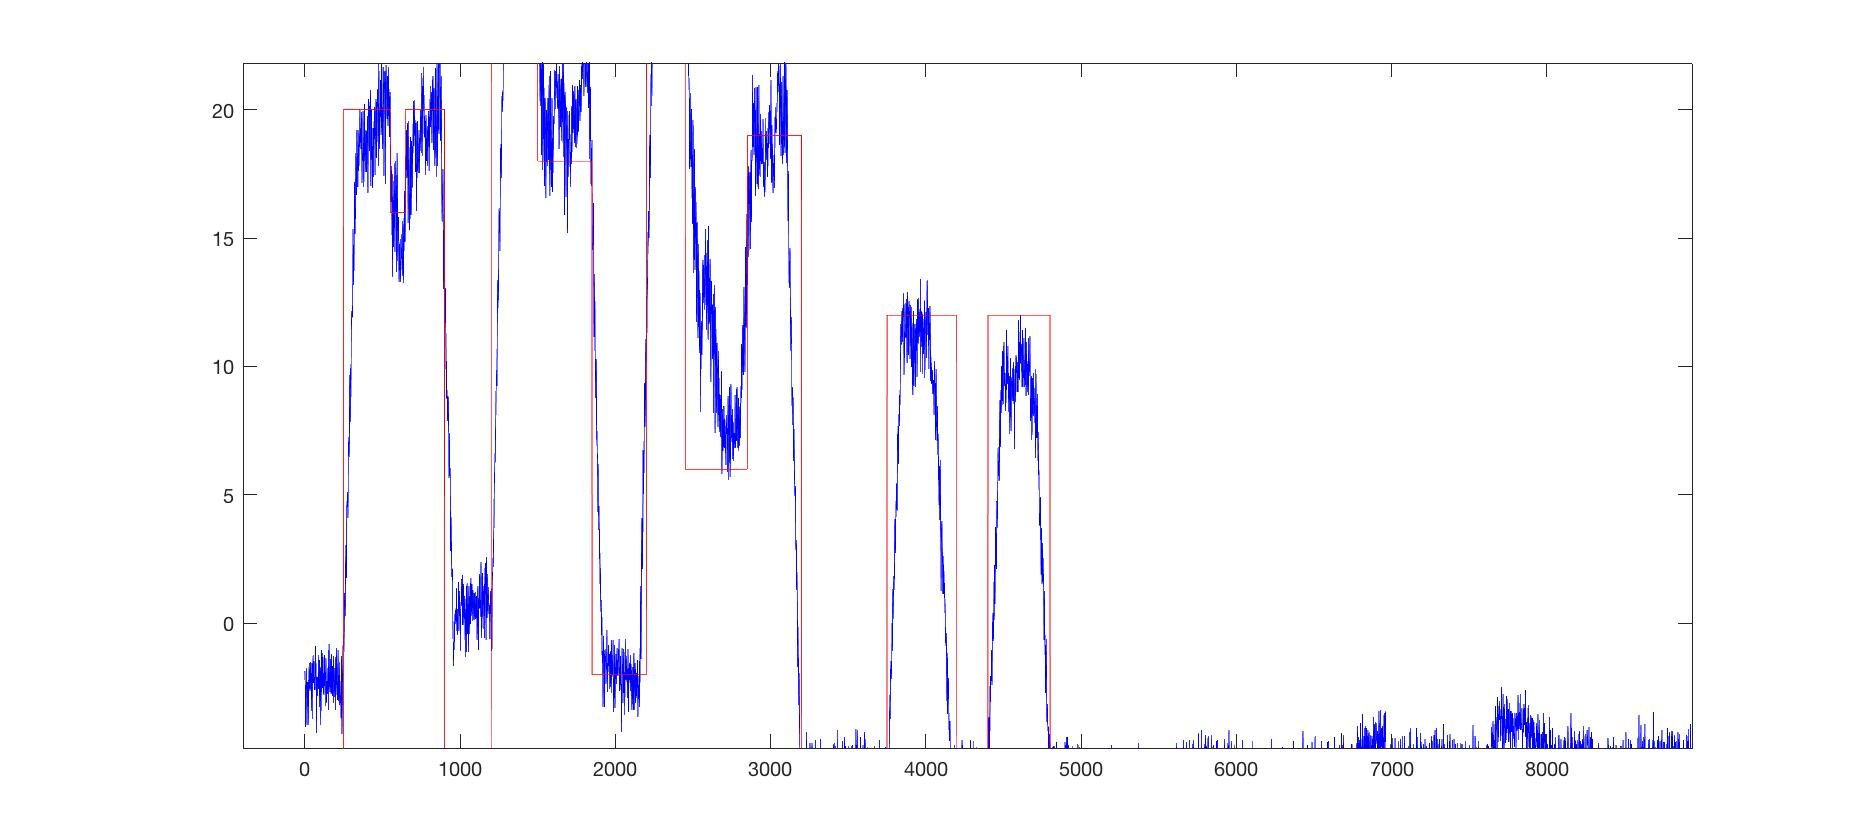
\includegraphics[height = 7.3 cm]{ofcom_ground_truth.jpg}
\caption{}
\label{fig:hvb}
\end{figure}


\section{Results: Distributed Estimation with Heaviside Basis}

\begin{figure}[h]
\centering
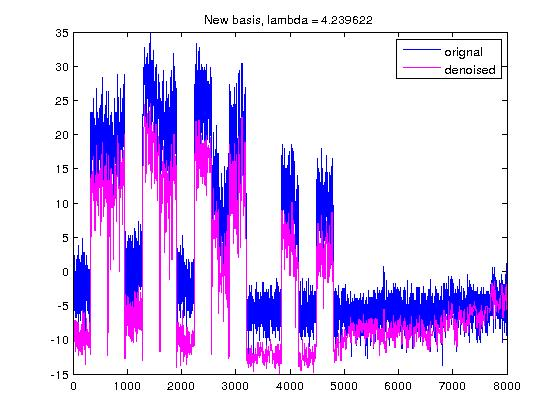
\includegraphics[height = 7.3 cm]{new_basis_ofcom_1.jpg}
\caption{Example of classification with OFCOM data, 35 changepoints}
\label{fig:hvb}
\end{figure}

\begin{figure}[h]
\centering
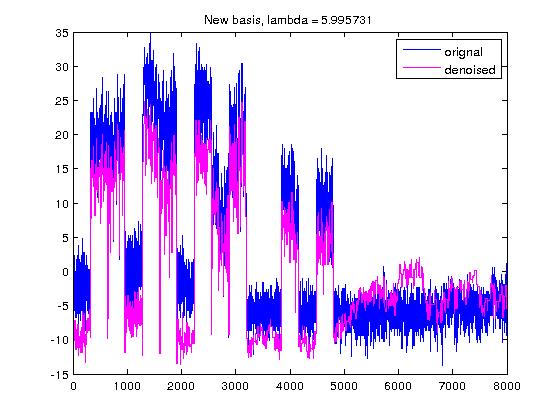
\includegraphics[height = 7.3 cm]{new_basis_ofcom_2.jpg}
\caption{Example of classification with OFCOM data, 55 changepoints}
\label{fig:hvb}
\end{figure}

\begin{figure}[h]
\centering
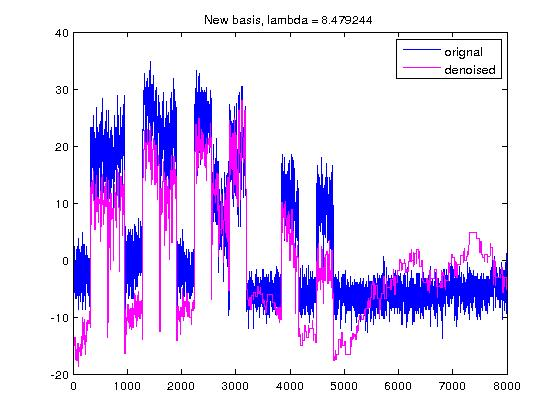
\includegraphics[height = 7.3 cm]{new_basis_ofcom_3.jpg}
\caption{Example of classification with OFCOM data, 35 changepoints}
\label{fig:hvb}
\end{figure}

\begin{figure}[h]
\centering
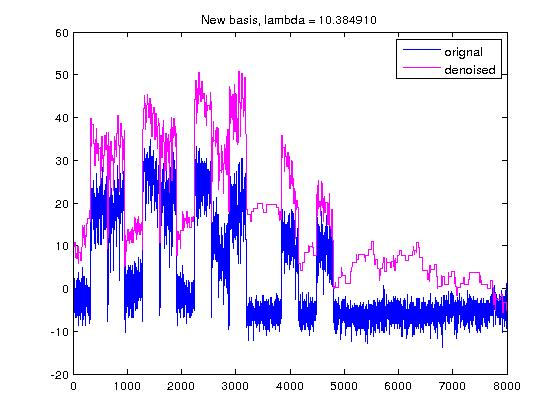
\includegraphics[height = 7.3 cm]{new_basis_ofcom_4.jpg}
\caption{Example of classification with OFCOM data, 55 changepoints}
\label{fig:hvb}
\end{figure}

These figures show that qualitatively, the distributed algorithm is capable of reconstructing the PSD in the TVWS band. This is good as it shows that a distributed algorithm is in principle capable of performing a large-scale reconstruction of PSD. It should be noted that to our knowledge, this is the only study using data sets this size. 

All these plots show significant co-linearlity between samples, so to address this we tried a distributed version of the Elastic Net. 

To more quantitatively asses how well our algorithm perfromed we...

\section{Compressive Estimation}

Some examples of the output of procedure \ref{alg:single-shot} are shown below, as applied to the OFCOM data set.

\begin{figure}[h]
\centering
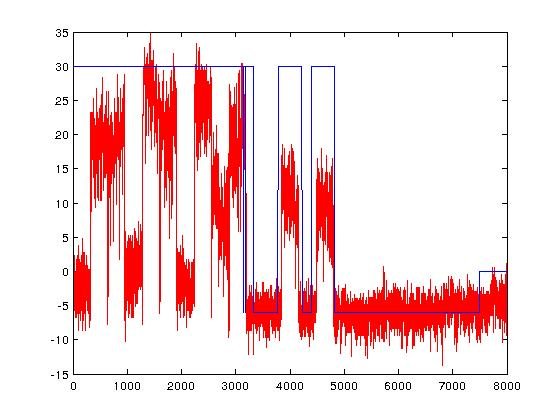
\includegraphics[height = 7.3 cm]{ofcom_classification1.jpg}
\caption{Example of classification with OFCOM data, 35 changepoints}
\label{fig:hvb}
\end{figure}

\begin{figure}[h]
\centering
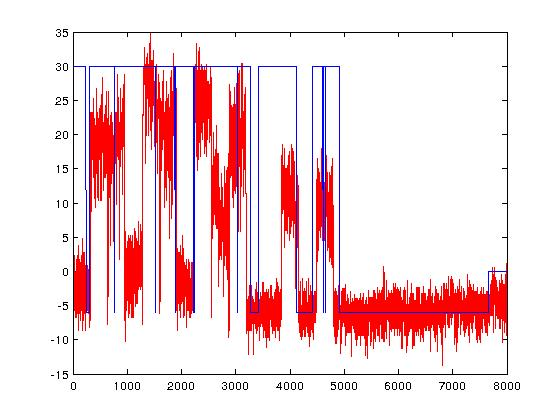
\includegraphics[height = 7.3 cm]{ofcom_classification.jpg}
\caption{Example of classification with OFCOM data, 55 changepoints}
\label{fig:hvb}
\end{figure}

\begin{figure}[h]
\centering
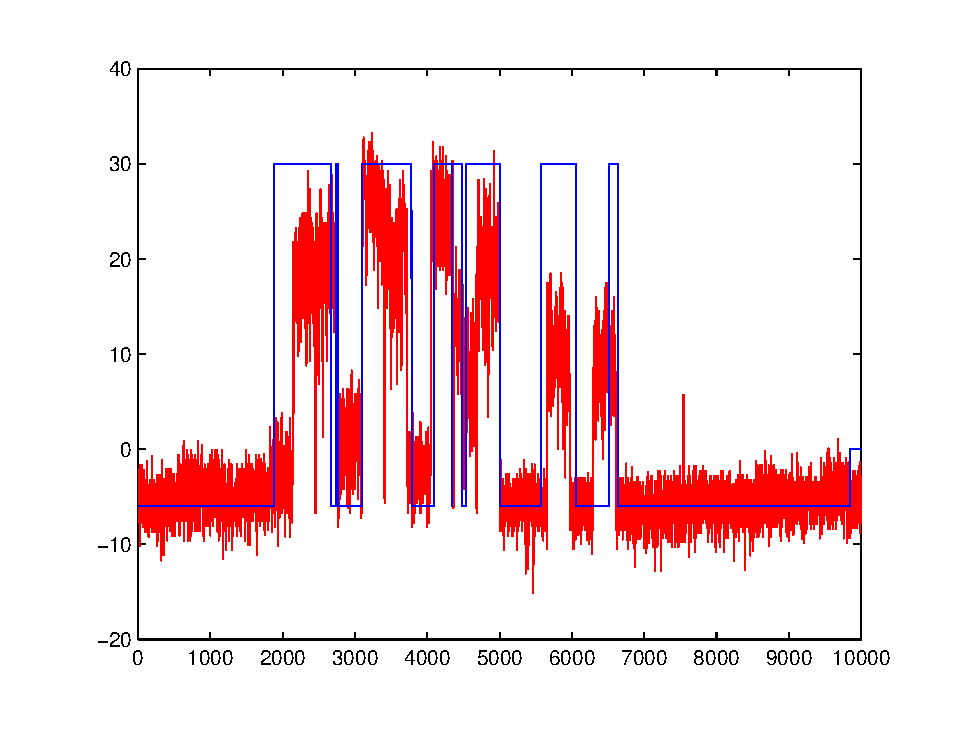
\includegraphics[height = 7.3 cm]{OFCOM5.eps}
\caption{Example of classification with OFCOM data, 35 changepoints}
\label{fig:hvb}
\end{figure}

\begin{figure}[h]
\centering
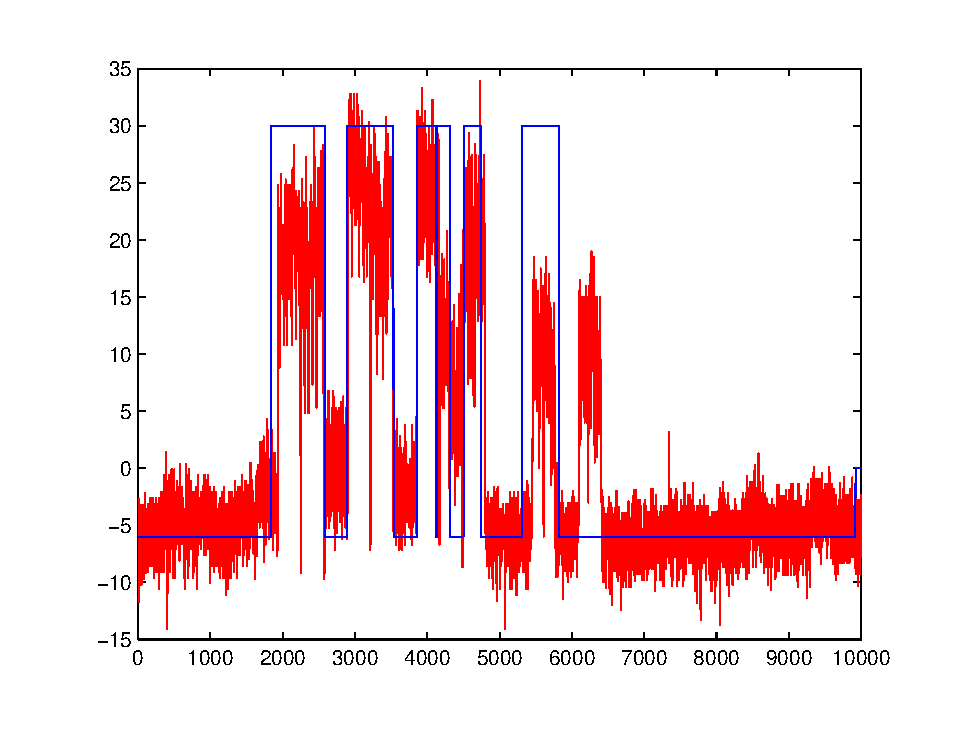
\includegraphics[height = 7.3 cm]{OFCOM6.eps}
\caption{Example of classification with OFCOM data, 55 changepoints}
\label{fig:hvb}
\end{figure}

\begin{figure}[h]
\centering
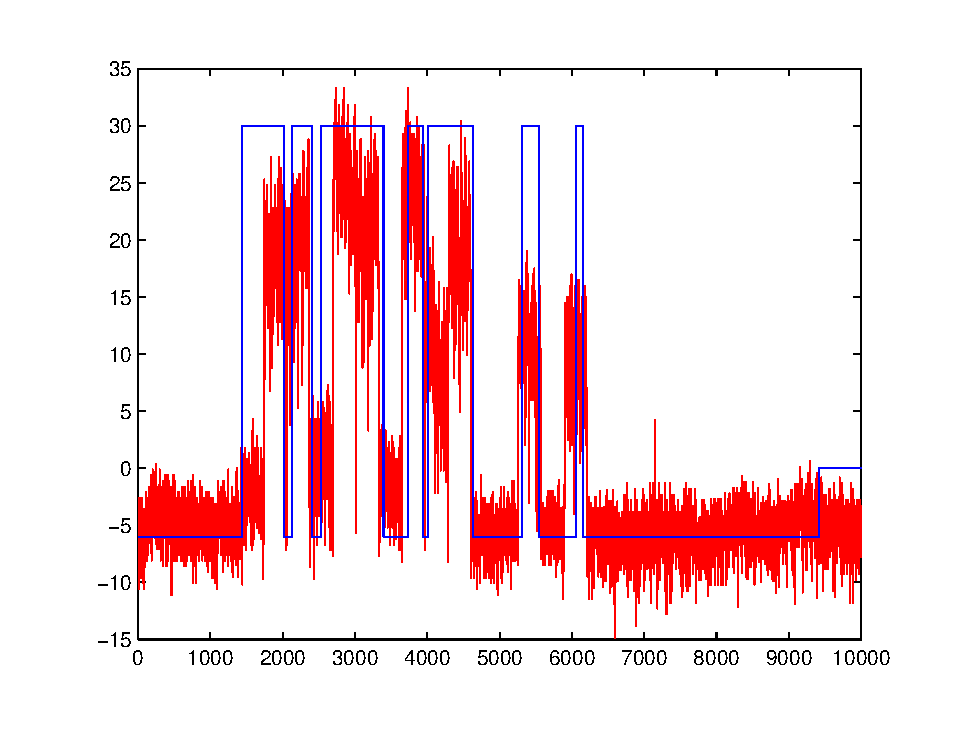
\includegraphics[height = 7.3 cm]{OFCOM7.eps}
\caption{Example of classification with OFCOM data, 35 changepoints}
\label{fig:hvb}
\end{figure}

\begin{figure}[h]
\centering
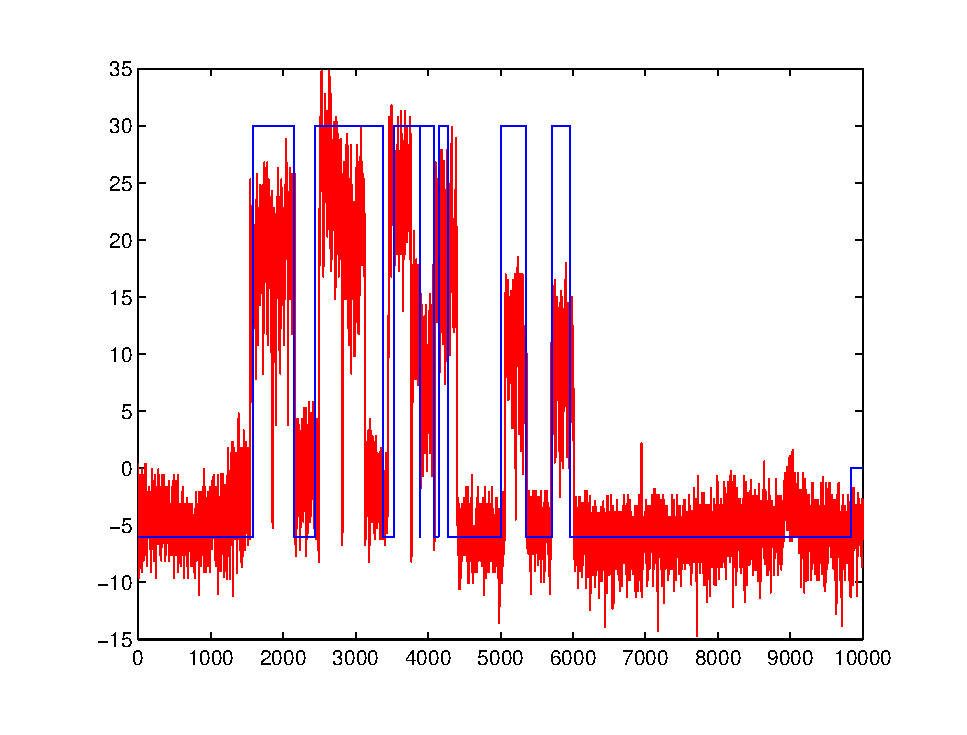
\includegraphics[height = 7.3 cm]{OFCOM8.eps}
\caption{Example of classification with OFCOM data, 55 changepoints}
\label{fig:hvb}
\end{figure}

\section{Conclusions}

\chapter{Group Testing}
\section{Introduction and notation}
This chapter outlines a contribution to the problem of group testing with non-identical probabilities. The material presented here was previously presented at Allerton 2014. 

Broadly, Group Testing is a sparse inference problem where the aim is to identify a small set of positive items contained within a much larger set of negative items, whilst aiming to minimise the number of times the items are checked (testes). As an example, consider trying to identify a sack containing coins weighing 1.1g from 9 other sacks containing coins weighing 1g, using an electric scale. This can be achieved in a single weighing of the coins: enuerate the bags, and take 1 coin  from bag 1, 2 from bag 2 etc. Weigh this set of coins. The total should be 55g, should all the coins weigh 1g. The ammont in 0.1g this ammount exceeds tells us which bag has the heavier coins. 

Group testing shares many features with compressive sensing. In particular, sparsity and randomness. In both scenarios, we are searching for the non-zero parts of a sparse vector; in both, random linear combinations of items are ued to reduce the number of tests/sample rate.

This chapter introduces the group testing problem, convers relevant literature on variations of this problem, and covers some applications of group testing. It defines the idea of group testing capacity, as well as algorithms which achieve this capacity. In particular we discuss an algorithm of Hwang, and illustrate how it achieves the capacity. 

We then extend the definition of probabilistic group testing to the case where the item probabilities are non-identical. We extend the definition of Group Testing capacity similarly. We then give an extension of the Laminar algorithm (presented in \cite{li5}) combining ideas from Hwang's algorithm to form a capacity achieving algorithm in the non-identical probabilites case.

We then present an analysis of said algorithm, proving that the algorith does indeed achieve capacity. 


\subsection{Group Testing}
Group Testing originated in the second world war because of the need to test all incoming conscriptees for syphilis. It would have been inefficient and expensive to test each soldier individually, as the rate for syphilis was only 10 per 100,000. Dorfman \cite{Dorfman1943}, considered the idea of pooling blood samples and testing the pooled samples for syphilis and only further testing the pools which come up positive.

A typical problem that can be solved by Group Testing is finding a counterfeit coin in a group of otherwise identical coins by weighing groups of coins on a pan balance. For example, given 80 coins known to contain a single counterfeit, which is lighter than the others, what is the minimum number of weighings needed to determine the counterfeit with certainty? You may get lucky and pick the counterfeit in the for the first go: but there's only a \(\frac{1}{80}\) chance of that happening. There's also no need to check all \(80 \choose 1\) combinations of pairs of coins. However, putting more than one coin on a pan reveals the same information  - it's better to weigh groups of coins against each other.

Choose the groups so that each weighing can distinguish between the hypothesis that the pans will balance, or than there will be a heavier pan i.e. split the initial group into 3 (27, 27, 26). Continue this process recursively, splitting the remaining group into 3 each time, until you have found the counterfeit. If the two groups of 27 balance initially, take a coin from one of those groups and add it to the group of 26 to make a power of 3. This won't add any new information (you know this coin is not counterfeit) and so won't affect the inference.

The Group Testing problem can be formalised as follows: a set of items is given, along with an upper bound on the number of defectives. The set is described as a vector, where if an item is 0 it is not defective and 1 if it is defective. Before the tests are run, the position of the 1's is unknown. 

To find the defective items, a query is run against a subset of \([n]\), where the answer is defined as follows:

\begin{equation}
A\left(S\right) = 1 \sum_{i} x_i \geq 1
\end{equation}

Note that the addition is the binary-or in the above summation. The goal of Group Testing is to minimise the number of tests required to reconstruct the defective set.

\subsubsection*{Algorithms}
An initial algorithm to consider is a simple binary search of the set to be tested. That is, given a set of size \(N = 2^r\) i.e a power of 2, we can recover a single defective in
\(\lceil{\log_2{N}}\rceil\) tests.

To do this, create a new set of size \(S = 2^{\lceil{\log_2{n}}\rceil}\) which is guaranteed to contain a defective. Label the items with integers, and test the items in the sets \({1,2,\ldots ,S/2}\) and \({S/2 + 1,\ldots ,S/2}\) separately. Then repeat the procedure on any groups which have a positive test. 

To see why this testing procedure takes at most \(\lceil{\log_2{n}}\rceil\) tests, note that the procedure defines a binary tree over subsets of the N items, and so the depth of this tree is \(\lceil{\log_2{N}}\rceil\).

For input sets with more than a single defective (say \(K\) defectives) the binary search algorithm can be repeated, and each time a defective is found it is removed from the set. The binary search is then repeated, but on a set of size \(N-1\). Using this procedure we are guaranteed to find all the defectives in 

\begin{equation}
K \lceil \log_2{N} \rceil \leq K\log_2{N} + K
\end{equation}

tests. However, this is a very inefficient algorithm: early sets are large and so are likely to contain a defective.

The above algorithms return, with certainty, after at most \(K\lceil \log_2{N\choose K}\rceil\) tests, the defective set. Much work has gone into combinatorial search algorithms, often more complex than those described above. 

This has been motivated by the analogy that the Group Testing problem can be considered a decoding problem where an experimenter receives a binary vector: 

\begin{equation}
y = \textbf{A}x
\end{equation}

\(y \in \{0,1\}^K, x \in \{0,1\}^N\), and wishes to decode the vector \(x\) to recover the defective set, subject to the constraints of the testing matrix \(\textbf{A}\). The matrix has to satisfy the property that the Boolean sum of any \(t\) columns was unique, and did not contain any other column in the matrix. These properties are known as seperability and disjunctness. 

\begin{figure*}[h]
\centering
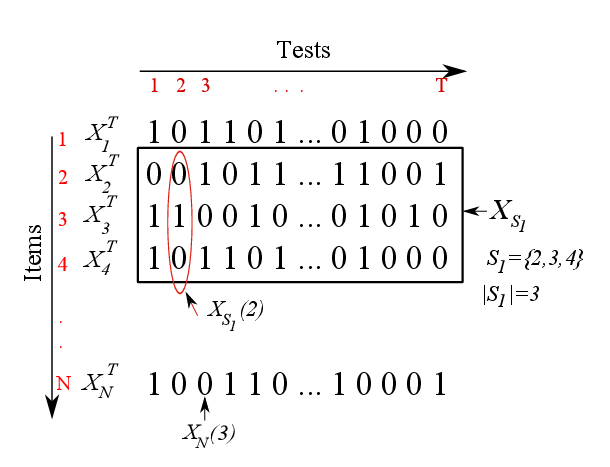
\includegraphics[height = 7 cm]{GTFat.png}
\caption{The Group Testing model: multiplication with a short, fat matrix \cite{atia2}}
\label{bayesiancs}
\end{figure*}

See \cite{du} for more a detailed introduction and analysis of the requisite algorithms.

\subsubsection*{Hwang's Algorithm}
In modern Coding Theory, there has been a move away from exlicit combinatorial algorithms which return the codeword with certainty, towards probabalisitic algorithms which return the correct codeword with an associated probability. The advantage of this has been the development of algorithms which can decode codes close to the Shannon capacity of the channel.

Similarly in Group Testing, the state of the art considers probabilistic algorithms instead of explicit combinatorial designs. 

The problems with the binary search algorithm (that initial groups are very large and are highly likely to contain a defective) above can be overcome by instead considering groups whose size is chosen so that the probability that the group will have a positive test is close to half. Equivalently, given a set of size \(N=2^r\) which are known to contain K defectives, in expectation a group of size \(\frac{K}{N}\) should contain a defective. 

Thus we can use fewer tests than predicted by simple repeated binary search, by testing 'pilot' groups of size roughly \(\frac{K}{N}\). Hwang \cite{Hwang1972} gives such an algorithm, and provides an upper bound on the number of tests required to recover the defective set.

The steps for the algorithm are:

\begin{enumerate}
\item If \(n \leq 2d-2\) then test every item individually. Otherwise set \(l = n - d + 1\) and define \(\alpha:=\log{\lceil \frac{l}{d}\rceil}\).
\item Test a group of size \(2^\alpha\). If the outcome is negative, the groups is good. Set \(n := n - 2^\alpha \) and go to 1. If the outcome is positive, then use binary splitting on the group to identify a defective and \(x\) good items. Set \(n := n - 1 -x \) and \(d:= d-1\) and go to 1.
\end{enumerate}

The upper bound on the number of tests is given by the following argument: as there are \(n \choose k\) possible sets of defectives, and in \(t\) tests at most \(2^t\) cases can be differentiated, \(\lceil \log_2{n \choose k} \rceil\) tests are needed. 

\subsubsection*{Bounds}
It has been previously believed that the success probability to recover the defective set given \(T\) tests was:

\begin{equation}
P\left(Success\right) \leq \frac{T}{\log_2{N \choose K}}
\end{equation}

However, a tighter upper bound has recently been found \cite{Aldridge2013} at:
%
\begin{equation}
P\left(Success\right) \leq \frac{2^T}{ {N \choose K} }
\end{equation}
%
i.e. the probability of success increases exponentially with the number tests, opposed to linearly. 

In the Group Testing literature there exists an 'adaptivity gap' - it seems that adaptive algorithms \textit{do} give a performance improvement over non-adaptive algorithms, in terms of the number of tests required to recover the defective set. This is discussed here, using Hwang's algorithm as a test bed.

Hwang's algorithm is guaranteed to succeed in:

\begin{equation}
T = \log_2{N\choose K} + K
\end{equation}

tests. The Combinatorial Orthogonal Matching Pursuit algorithm, considered in \cite{Chan2011}, is guaranteed to recover the defective set with probability \(N^{-\delta} \) in
%
\begin{equation}
T = \left(\left(1+\delta\right)e\right)K\ln{N}
\end{equation}
%
tests. For all \(N\) and \(K)\) we have:
%
\begin{equation}
K\log_2{\frac{N}{K}} \leq \log_2{N \choose K} \leq K \log_2{\frac{Ne}{K}}
\end{equation}
%
which follows from well-know bounds on binomial coefficients. This allows a contrast between the asymptotic bounds of previous algorithms to be considered in this section. We see that, the regime where \(K = N^{1-\beta}\), Hwang's algorithm succeeds with:
%
\begin{equation}
T = \beta K \log_2{N} + K\left(\log_2{e} + 1\right)
\end{equation}
\label{hwangbound}
%
tests, whilst the COMP algorithm succeeds with:
%
\begin{equation}
1.88\left(1+\delta\right)K\log_2{N}
\end{equation}
\label{compbound}
%
tests. It's worthwhile to contrast these results, to gain some insight into the problem. \ref{hwangbound} suggests that for very sparse problems (\(\beta\) tending towards 1) that Hwang's adaptive algorithm will outperform a simmilar non-adaptive algorithm. Even though the two procedures have the same complexity, they have different constants (1 v,s 1.88 in the sparse case). Thus, there are asymptotic gains (in terms of the number of tests required to recover the defective set) which are offered by adaptive algorithms, and not by non-adaptive algorithms.

These ideas can be summarised in the idea of a \textit{capacity} for Group Testing \cite{Baldassini2013}. That is, there is a constant \(C\) such that a sequence of Group Testing algorithms with \( K = \omega\left(N\right)\) will succeed with probability tending to 1. This allows different noise, and dilution models to be considered so that a more complete characterisation of the structural properties of Group Testing is revealed.
 
\subsubsection{Comparison to Compressive Sensing}
The goal of Coding Theory is given a vector \(x \in \mathbb{F}^m\), where \(\mathbb{F}\) is some finite-field, is to construct a 'code-book' \(C\) which produces a vector \(y \in \mathbb{F}^n\), \(n > m\), so that the original vector may be transmitted over a noisy-channel with vanishing error probability. This problem is structurally similar to the Compressive Sensing and Group Testing problems, but in reverse. In CS and GT we're given 'short' vector, and we wish to infer the 'longer' one satisfying the constraint that we seek the sparsest vector, under some conditions on the matrix \(\Phi\). This suggests that there may be some Information-theoretic framework uniting all three disciplines. 

In \cite{Emma} Tao and Candes consider the CS problem as one of error correction of a linear code: however in this case the codewords are drawn from \(\mathbb{R}^m\) as opposed to a finite alphabet more common in Coding Theory. This is done by considering \(\Phi\) as the parity check matrix of a linear code and the signal x as the error pattern. Linear programming can then be viewed as a method for decoding. 

Group testing is a combinatorial variant of Compressive Sensing, where the sensing matrix is a binary matrix. The matrix represents combinations (or pools) of items, such that a 1 in the \(i^{th}\) row and \(j^{th}\) column means that  the \(i^{th}\) item is tested in the \(j^{th}\) pool. The goal of Group testing can then be seen as designing testing pools so to accurately reconstruct the sparse set of interesting items. 

In Group Testing, instead of the sensing matrix being to subject to coherence constraints such as those above, the sensing matrices have the property that the support of any column is not contained in the union of the supports of any t other columns. Thus a t-disjunct matrix defines a group testing scheme which an identify any defective set up to size t.

The analogue between Group Testing and Coding is even closer, as GT explicitly considers signals and matrices from Binary alphabets. That is, Group Testing is a closer cousin of Coding Theory than Compressive Sensing, in a sense the inverse problem as in both Coding and Group Testing we are working over a finite field. This is encouraging, as it could allow the reconstruction of the defective set via methods developed in Coding Theory. There has been some work done on this, \cite{Sejdinovic2010} considers the noisy Group Testing problem and the reconstruction of the defective set via belief propagation whilst \cite{Wadayama} gives explicit theorems on conditions for the recovery of the defective set for the case of the binary symmetric channel. \cite{Baldassini2013} takes this further and finds the capacity of Group Testing for a number of cases. 

\subsection{The Probabilistic group testing problem}
Group testing is a sparse inference problem, first introduced by Dorfman \cite{dorfman} in the context of testing for rare diseases.
Given  a large population of items $\setP$,
indexed by \( \{1, \ldots N\}\), where
some small fraction of the items are interesting in some way, how can we find the interesting items efficiently? 

We perform a sequence of $T$ pooled tests defined by test sets $\setX_1, \ldots, \setX_T$, where each $\setX_i \subseteq \setP$. 
We represent the interesting (`defective') items by 
a random vector $\vc{U} = ( U_1, \ldots, U_N)$, where $U_i$ is the indicator of the event that item $i$ is defective. 
For each test $i$, we jointly 
test all the items in $\setX_i$, and the outcome $y_i$ is `positive' ($y_i = 1$) if and only if any item in $\setX_i$ is defective. In other words, 
$y_i = \II \left( \sum_{j \in \setX_i} U_j \right)$, since for simplicity we are  considering the noiseless case. Further, in this paper, we restrict our attention to
 the adaptive case, where we choose test set
$\setX_i$ based on a knowledge of sets $\setX_1, \ldots, \setX_{i-1}$ and outcomes $y_1, \ldots, y_{i-1}$. The group testing problem requires us to infer $\vc{U}$ with high
probability given a low number of tests $T$.

Since Dorfman's paper \cite{dorfman}, there has been considerable work on the question of how to design the sets $\setX_i$ in order to minimise the number of tests $T$
required. In this context, we briefly mention so-called combinatorial designs (see \cite{du, malyutov} for a summary, with \cite{malyutov} giving invaluable
references to an extensive body of Russian work in the 1970s and 1980s). Such designs typically aim to ensure that 
set-theoretic properties known as disjunctness
and separability occur. In contrast, for simplicity of analysis, as well as  performance of optimal order, it is possible to consider random designs. Here sets $\setX_i$ are chosen
at random, either using constructions such as independent Bernoulli designs \cite{atia, johnsonc8, johnson33} or more sophisticated  random designs based on LDPC codes \cite{Wadayama}. 

Much previous work has focussed on the Combinatorial group testing problem, where there are a fixed number of defectives $K$, and the defectivity vector $\vc{U}$ is chosen uniformly among all
binary vectors of weight $K$. In contrast, in this paper we study a Probabilistic group testing problem as formulated
for example in the work of Li et al. \cite{li5}, in that we suppose 
 each item is defective  independently with probability \(p_i\), or equivalently take $U_i$ to be independent Bernoulli($p_i$).

This Probabilistic framework, including non-uniform priors, is natural for many applications of group testing.
For example, see \cite{atia2}, the cognitive radio problem can be formulated in terms of  a population
 of communication bands in frequency spectra with some (unknown) occupied bands you must not utilise. Here, the values of $p_i$ may be chosen
 based on some database of past spectrum measurements or other prior information. Similarly, as in Dorfman's original work  \cite{dorfman} or more recent 
research \cite{shental} involving screening for genetic conditions, values of
$p_i$ might summarise prior information based on a risk profile or  family history.
%
\subsection{Group testing capacity}
%
It is possible to characterize performance tradeoffs in group testing 
 from an information-theoretic point of view -- see for example \cite{atia, johnsonc10, johnson33, tan}. These papers have focussed on group testing as a channel coding problem, 
with \cite{atia, tan}
explicitly calculating the mutual information.
The paper \cite{johnsonc10} defined the capacity of a Combinatorial group testing procedure, which characterizes the number of bits of information
about the defective set which we can learn per test. We give a more general definition here,
which covers both the Combinatorial and Probabilistic cases.
%
\begin{definition} \label{def:capacity} Consider a sequence of group testing problems where the $i$th problem
has defectivity vector  $\vc{U}^{(i)}$, and consider algorithms which are given $T(i)$ tests.
We refer to a constant $C$ as the (weak) group testing capacity if for any $\epsilon > 0$:
  \begin{enumerate}
    \item any sequence of algorithms with
      \begin{equation} \label{eq:lower}
        \liminf_{i \tends} \frac{ H(\vc{U}^{(i)}) }{T(i)} \geq C+ \epsilon,
      \end{equation}
      has success probability $\pr(\textrm{suc})$ bounded away from 1,
    \item and there exists a sequence of algorithms with
      \begin{equation} \label{eq:upper}
        \liminf_{i \tends} \frac{H(\vc{U}^{(i)}) }{T(i)}  \geq C - \epsilon
      \end{equation}
      with success probability $\pr(\suc) \rightarrow 1$.
  \end{enumerate}
\end{definition}
%
\begin{remark}
In the Combinatorial case of $K$ defective items with all defective sets equally
likely, $ H(\vc{U}) = \log_2 \binom{N}{K}$, which is the term found in the denominator in \cite[Eq. (1) and (2)]{johnsonc10}. In the Probabilistic case (as in \cite{li5}) 
 we know $H(\vc{U}) = -\sum_{i=1}^N h(p_i)$ where $h(t) = -t \log_2 t - (1-t) \log_2(1-t)$ is the binary entropy function. 
\end{remark}
%
\begin{remark} If for $ \liminf_{i \tends} \frac{ H(\vc{U}^{(i)}) }{T(i)} \geq C+ \epsilon$, the success probability 
$\pr(\suc) \rightarrow 0$ we say that $C$ is the strong group testing capacity, following standard terminology in information
theory. Such a result is referred to as a strong converse.
\end{remark}

\subsection{Main results}

The principal contribution of \cite[Theorem 1.2]{johnsonc10} was the following result:
%
\begin{theorem}[\cite{johnsonc10}] \label{thm:mainold}
The strong capacity of the adaptive noiseless Combinatorial group testing problem
  is  $C = 1$,
  in any regime such that $K/N \rightarrow 0$.
\end{theorem}
%
This argument came in two parts. First, in \cite[Theorem 3.1]{johnsonc10} the authors  proved a new
upper bound on success probability 
\begin{equation} \label{eq:bja} \pr(\suc) \leq \frac{2^T}{\binom{N}{K}}, \end{equation} which implied a strong converse ($C \leq 1$). This was complemented 
by 
showing that, in the Combinatorial case, an algorithm based on 
Hwang's Generalized Binary Splitting Algorithm (HGBSA) \cite{hwang}, \cite{du} is essentially optimal in the required sense,
showing that $C=1$ is achievable.


It may be useful to characterize the Probabilistic group testing problem in 
terms of the effective sparsity $\mu^{(N)}: = \sum_{i=1}^N p_i$. In particular, if the $p_i$ are (close to) identical, we would expect performance similar to that in the Combinatorial
case with $K = \mu^{(N)}$ defectives. As in \cite{johnsonc10}, we  focus on asymptotically sparse cases, where $\mu^{(N)}/N \rightarrow 0$ (in contrast, Wadayama
\cite{} considered a model where $p_i$ are identical and fixed).
The main result of the present paper is Theorem \ref{thm:main}, stated and proved in Section \ref{sec:main} below, which implies the 
following  Probabilistic group testing version of Theorem \ref{thm:mainold}.
 %
\begin{corollary} \label{cor:main}
 In the case where $p_i \equiv p$, the weak capacity of the adaptive noiseless Probabilistic group testing problem
  is  $C = 1$, in any regime such that $\mu^{(N)}/N \rightarrow 0$ and $\mu^{(N)} \rightarrow \infty$.
  \end{corollary}



Again we prove our main result Theorem \ref{thm:main} using complementary bounds on both sides. First in Section \ref{sec:ub} we recall
 a universal upper bound on success probability, Theorem \ref{thm:upper}, taken from
\cite{li5}, which implies a weak converse.   In \cite{li5}, Li et al. introduce
the Laminar Algorithm for Probabilistic group testing.  
In Section \ref{sec:algo} we propose a refined version of this Laminar Algorithm, based on Hwang's HGBSA \cite{hwang}, which is
analysed in Section \ref{sec:main}, and shown to imply performance close to optimal in the sense of capacity.

\section{Algorithms and existing results}

\subsection{Upper bounds on success probability} \label{sec:ub}

Firstly \cite[Theorem 1]{li5} can be restated to give the following
upper bound on success probability:
%
\begin{theorem} \label{thm:upper}
Any Probabilistic group testing algorithm using $T$ tests with noiseless measurements has success probability satisfying
$$ \pr(\suc) \leq \frac{T}{H( \vc{U})}.$$
\end{theorem}

Rephrased in terms of Definition \ref{def:capacity}, this tells us that the weak capacity of noiseless Probabilistic 
group testing is $\leq 1$. The logic is as follows; if the capacity were
$1 + 2 \epsilon$ for some $\epsilon > 0$, then there would exist a sequence of algorithms with $H(\vc{U}^{(i)})/T(i) \geq 1 + \epsilon$ with success probability tending to 1.
However, by Theorem \ref{thm:upper}, any such algorithms have $\pr(\suc) \leq 1/(1+\epsilon)$, meaning that we have 
established that a weak converse holds.

\begin{remark}
It remains an open and interesting problem to prove an equivalent of \eqref{eq:bja} as in \cite[Theorem 3.1]{johnsonc10}. That is we hope to find an upper bound
on success probability in a form  which implies a strong converse, and hence that the strong capacity of Probabilistic group
testing is equal to 1.
\end{remark}

\subsection{Binary search algorithms}

The main contribution of this work is  to describe and analyse algorithms that will find the defective items.
In brief, we can think of Hwang's HGBSA algorithm as dividing the population $\setP$ into search sets $\setS$. First, all the items in a search set $\setS$ are tested together,
using a test set $\setX_1 = \setS$. If the result is negative
($y_1 = 0$), we can be certain that $\setS$ contains no defectives. However, if the result is positive ($y_1 = 1$),  $\setS$ must contain at least one defective.

If $y_i = 1$, we can be guaranteed to find at least
one defective, using the following binary search strategy.  
We  split the   set $\setS$ in two, and test the `left-hand' set, say $\setX_{2}$. If $y_{2} = 1$, then we know that $\setX_{2}$ contains at least one defective.
If $y_{2} = 0$, then $\setX_{2}$ contains no defective, so we can deduce that $\setS \setminus \setX_2$ contains at least one defective. By repeated use of this strategy, we are 
guaranteed to find a succession of nested sets which contain at least one defective, until $\setX_i$ is of size 1, and we have isolated a single defective item.

However this strategy may not find every defective item in $\setS$. To be specific, it is possible that at some stage
both the left-hand and right-hand sets contain a defective. The Laminar Algorithm of \cite{li5} essentially deals with this by testing 
both sets. However, we believe that this is inefficient, since typically both sets will not contain a defective. Nonetheless, the Laminar Algorithm satisfies
 the following  performance guarantees  proved in \cite[Theorem 2]{li5}: 
%
\begin{theorem} \label{thm:lower}
The expected number of tests required by the Laminar Algorithm \cite{li5}  is $\leq 2 H(\vc{U}) + 2 \mu$. Under a technical condition (referred to as non-skewedness), the
success probability can be bounded by $\pr(\suc) \geq 1- \epsilon$ using $T = (1+ \delta) (2^{\Gamma + \log_2 3} + 2) H(\vc{U})$ tests, where $\Gamma$ is defined implicitly
in terms of $\epsilon$, and $\delta \geq 2 e - 1$.
\end{theorem}

Ignoring the $\Gamma$ term, and assuming the non-skewedness condition holds,
 this implies that (using the methods of \cite{li5}) $T =  2 e (3 + 2) H(\vc{U}) = 10 e H(\vc{U})$ tests are required to guarantee convergence to $1$
of the success probability. In our language, this implies a lower bound of $C \geq 1/(10 e) = 0.0368$. Even ignoring the analysis of error probability, the fact that the expected number
of tests is $\leq 2 H(\vc{U}) + 2 \mu$ suggests that we cannot hope to achieve $C > 1/2$ using the Laminar Algorithm.
%
\subsection{Summary of our contribution} \label{sec:algo}

\begin{figure}
\begin{algorithmic}
 %\SetAlgoLined % For previous releases [?]
 \State{A Set \(S\) of \(\lvert S \rvert = n\) items, \(\mu\) of which are actually defective in expectation, a probability vector \( \vec{p}^{\left(n\right)} \) describing each item's independent probability of being defective, and a cutoff \(\theta\)}
 \State{\textbf{Returns}The set of defective items}
 Discard items with \(p_i \leq \theta\)
 \\
 Sort the remaining items into \(B\) bins, collecting items together with \(p_i \in \left[1/2C^r,1/2C^{r-1}\right)\) in bin \(r\).
 \\
 Sort the items in each bin into sets s.t. the (normalised) probability of each set is less than \(1/2\).
 \\
 Test each set in turn
 \\
   	\If{The test is positive}{Arrange the items in the set on a Shannon-Fano/Huffman Tree and search the set for all the defectives it contains}
	\EndIf

\end{algorithmic}
 \caption{Algorithm for the non-iid group testing problem}
\end{figure}

The main contribution of our paper is a refined version of the Laminar Algorithm, summarised above, and an analysis resulting in tighter error bounds as formulated in Proposition \ref{prop:overall} (in terms of expected number of tests) and Theorem \ref{thm:main} (in terms
of error probabilities).
The  key ideas are:
\begin{enumerate}
\item To partition the population $\setP$ into search  sets  $\setS$ containing items which have similar probabilities,
expressed through the Bounded Ratio Condition \ref{cond:ratio}. This is discussed in Section \ref{sec:boundedratio}, and optimised in the proof
of Proposition \ref{prop:overall}.
\item The way in which we deal with sets $\setS$ which contain more than one defective, as discussed in Remark \ref{rem:algo} below. Essentially we do not backtrack after each test by
testing both left- and right-hand sets, but only backtrack after each defective is found.
\item To discard items which have probability below a certain
threshold, since with high probability none of them will be defective. This is an idea introduced in \cite{li5} and discussed
in Section \ref{sec:discard}, with a new bound given in Lemma \ref{lem:thresh}.
\item  Careful analysis in Section \ref{sec:expectation} of the properties of search sets $\setS$ gives Proposition \ref{prop:overall}, which shows that the expected number of tests required can
be expressed as $H(\vc{U})$ plus an error term. In Section \ref{sec:main},
we give an analysis of the error probability using Bernstein's inequality, Theorem \ref{thm:bernstein}, allowing us to
prove Theorem \ref{thm:main}.
\end{enumerate}
%


\subsection{Wider context: sparse inference problems}

Recent work \cite{aksoylar,tan} has shown that many arguments and bounds hold in a common framework of sparse inference
which includes group testing and compressive sensing.

Digital communications, audio, images, and text are examples of data sources we can compress. We can do this, because these data sources are sparse: they have fewer degrees of freedom than the space they are defined upon. 
For example, images have a well known expansion in either the Fourier or Wavelet bases. The text of an English document will only be comprised of words from the English dictionary, and not all the possible strings from the space of strings made up from the characters \(\{a, \ldots, z \}\). 

Often, once a signal has been acquired it will be compressed. However, the compressive sensing paradigm introduced by
\cite{Candes2006,donoho2} shows that this isn't necessary. In those papers it was shown that a 'compressed' representation of a signal could be obtained from random linear projections of the signal and some other basis (for example White Gaussian Noise). The question remains, given this representation how do we recover the original signal? For real signals, a simple linear programme suffices.
Much of the work in this area has been couched in terms of the sparsity of the signal and the various bases the signal can be represented in (see for example \cite{Candes2006,donoho2}). 


\section{Analysis and new bounds}

\subsection{Searching a set of bounded ratio} \label{sec:boundedratio}

Recall that we have a population $\setP$ of items to test, each with associated probability of defectiveness $p_i$.
The strategy of the proof is to partition $\setP$ 
 into search sets $\setS_1, \ldots, \setS_G$, each of which contains items which have
comparable values of $p_i$.

\begin{condition}[Bounded Ratio Condition] \label{cond:ratio}
Given $C \geq 1$, say that a set $\setS$ satisfies the Bounded Ratio Condition with constant $C$ if
\begin{equation} \label{eq:ratio} \max_{i,j \in \setS} \frac{p_j}{p_i} \leq C.\end{equation} \end{condition}
%
(For example clearly if $p_i \equiv p$, any set $\setS$ satisfies the condition for any $C \geq 1$).
%
\begin{lemma} \label{lem:sfstep}
Consider a set $\setS$ satisfying the Bounded Ratio Condition  with constant $C$
and write $P_{\setS} = \sum_{j \in \setS} p_j$.
In a  Shannon--Fano tree for the probability distribution $\ol{p}_i := p_i/P_{\setS}$, each item has length $\ell_i^{(\setS)}$
bounded by
\begin{equation} \label{eq:depth} \ell_i^{(\setS)} \leq \ell_{\max}^{(\setS)} := \frac{h(\setS)}{P_{\setS}} + \log_2  C + \log_2  P_{\setS} + 1,\end{equation}
where we write $h( \setS) :=  -\sum_{j \in \setS} p_j \log_2  p_j$.
\end{lemma}
\begin{proof} Under the Bounded Ratio Condition, for any $i$ and $j$, we know that by taking logs of \eqref{eq:ratio}
$$ -\log_2 p_i \leq - \log_2 p_j + \log_2 C.$$
Multiplying by $p_j$ and summing over all $j \in \setS$, we obtain that
\begin{equation} \label{eq:setbd} -P_{\setS} \log_2 p_i \leq h(\setS) + P_{\setS} \log_2 C.\end{equation}
Now, the Shannon--Fano length of the $i$th item is
\begin{eqnarray}
 \ell_i^{(\setS)}  = \lceil -\log_2 \ol{p}_i \rceil 
& \leq &  -\log_2 p_i + \log_2 P_{\setS} + 1 \label{eq:lengthbd} \\
& \leq  & \left(\frac{h(\setS)}{P_{\setS}} + \log_2 C \right) + \log_2 P_{\setS} + 1. \nonumber
\end{eqnarray}
and the result follows by \eqref{eq:setbd}.
\end{proof}

Next we describe our search strategy:

\begin{remark} \label{rem:algo}
Our version of the algorithm will find every defective in a set $\setS$. We start as before by testing every item in $\setS$ together. If this test is negative, we are done.
Otherwise, if it is positive, we can perform binary search as above to find one defective item, say $d_1$. Now, test every item in $\setS \setminus \{ d_1 \}$ together.
If this test is negative, we are done, otherwise we repeat the search step on this smaller set, to find another defective item
$d_2$, then we test $\setS \setminus \{ d_1, d_2 \}$ and so on.

We think of the algorithm as repeatedly searching a binary tree. Clearly, if the tree has depth bounded by $\ell$, then the search will take $ \leq \ell$ tests to find one defective. In total, 
if the set contains $U$ defectives, we need to repeat $U$ rounds of searching, plus the final test to guarantee that the set contains no more defectives, so will use $\leq \ell U + 1$ tests.
\end{remark}

\begin{lemma} \label{lem:expset}
 Consider a search set $\setS$ satisfying the Bounded Ratio Condition  and write $P_{\setS} = \sum_{j \in \setS} p_j$.
If (independently) item $i$ is defective with probability $p_i$, 
we can recover  all defective items in the set using $T_\setS$ tests, where $\ep T_\setS \leq T_{\bd}(\setS)$ for
\begin{equation} \label{eq:tbds}
 T_{\bd}(\setS) :=  h(\setS) +  P_{\setS} \log_2 C +  P_{\setS} \log_2 P_{\setS} + P_\setS + 1. \end{equation}
\end{lemma}
\begin{proof}
Using the algorithm of Remark \ref{rem:algo}, laid out on the Shannon-Fano tree constructed in Lemma \ref{lem:sfstep}, we are guaranteed  to find every defective.
The number of tests to find one defective thus corresponds to the depth of the tree, which is bounded by  $\ell_{\max}^{(\setS)}$ given in \eqref{eq:depth}.

Recall that we write $U_i$ for the indicator of the event that the $i$th item is defective, $U_{\setS} = \sum_{i \in \setS} U_i$ and 
$l_i^{(\setS)}$ for the length of the word in the Shannon Fano tree. As discussed in Remark \ref{rem:algo}
this search procedure will take 
\begin{eqnarray}
T_\setS & = &  1 + \sum_{i \in \setS} U_i \ell_i^{(\setS)} \nonumber \\
& = &  \sum_{i \in \setS} p_i \ell_i^{(\setS)} + 1 + \sum_{i \in S} \ell_i^{(\setS)} (U_i - p_i)  \nonumber \\
& \leq & \sum_{i \in \setS} p_i \ell_{\max}^{(\setS)} +  1 + \sum_{i \in \setS} V_i^{(\setS)}  \nonumber \\
& =  &  P_{\setS} \ell_{\max}^{(\setS)} +  1 + \sum_{i \in S} V_i^{(\setS)} \nonumber \\
& \leq  & T_{\bd}(\setS) + \sum_{i \in S} V_i^{(\setS)} 
\mbox{ \;\; tests.} \label{eq:testsperdef} \end{eqnarray}
Here we write $V_ i^{(\setS)} = \ell_i^{(\setS)} (U_i - p_i)$, which has expectation zero, and \eqref{eq:testsperdef} follows using the expression for 
$\ell_{\max}^{(\setS)}$ given in   Lemma \ref{lem:sfstep}.
\end{proof}

\subsection{Discarding low probability items} \label{sec:discard}

As in \cite{li5}, we use a probability threshold $\theta$, and write $\setP^*$ for the population having removed items with $p_i \leq \theta$.
If an item lies in $\setP \setminus \setP^*$ we do not 
test it, and simply mark it as non-defective. This truncation operation gives an error if and only if some item in $\setP \setminus \setP^*$ is defective.
By the union bound, 
this truncation operation contributes a total of $\pr( \mbox{$\setP \setminus \setP^*$ contains a defective}) \leq  \rho := \sum_{i=1}^n p_i \II(p_i \leq \theta)$ to the error probability.



\begin{lemma} \label{lem:thresh}
Choosing $\theta(P_e)$ such that  
\begin{equation} \label{eq:thetadef}
-\log_2 \theta(P_e) = \min\left( \log_2  \left( \frac{2n}{P_e} \right), \frac{2 H( \vc{U})}{P_e} \right)
\end{equation}
ensures that  
\begin{equation}
\pr( \mbox{ $\setP \setminus \setP^*$ contains a defective} ) \leq P_e/2. \label{eq:setpstar} \end{equation} \end{lemma}
\begin{proof}
The approach of \cite{li5} is essentially to bound $\II(p_i \leq \theta) \leq \theta/p_i$ so that
$\rho = \sum_{i=1}^n p_i \II(p_i \leq \theta) \leq \sum_{i=1}^n p_i (\theta/p_i) = n \theta$. Hence, choosing a threshold
of $\theta = P_e/(2n)$ guarantees the required bound on $\rho$.

We combine this with another bound, constructed using a different function:
 $\II(p_i \leq \theta) \leq (-\log_2 p_i)/(-\log_2 \theta)$, so that
$$ \rho = \sum_{i=1}^n p_i \II(p_i \leq \theta) \leq \sum_{i=1}^n p_i  \left( 
\frac{-\log_2 p_i}{-\log_2 \theta } \right) \leq \frac{H( \vc{U})}{-\log_2 \theta},$$ 
so we deduce the result. \end{proof}

\subsection{Searching the entire set} 

Having discarded items with $p_i$ below
this probability threshold $\theta$ and given bounding ratio $C$,
we create a series of bins. We collect together items with probabilities $p \in [1/2,1]$ in bin 0,
$p \in [1/(2C), 1/2)$ in bin 1, items with probabilities $p \in [1/(2C^2), 1/(2C))$ in bin 2, \ldots, and items with probabilities $p \in 
[1/(2C^B), 1/(2C^{B-1}))$ in bin $B$.

The probability threshold $\theta$ means that
there will be a finite number of such bins, with the index $B$ of the last bin defined by the fact that $1/(2C^B) \leq
\theta < 1/(2C^{B-1})$, meaning that $(B -1) \log_2 C < - \log_2 (2 \theta)$, so
\begin{equation} \label{eq:bincount} B \leq  \frac{ - \log_2 (2 \theta)}{\log_2 C} + 1. \end{equation}

We split the items in each bin into search sets $\setS_i$, motivated by the following definition:

\begin{definition} \label{def:full}
A set of items \( \setS \) is said to be full if $P_{\setS} = \sum_{i \in \setS} p_i \geq \frac{1}{2}$.
\end{definition}

Our splitting procedure is as follows: we create a list of
possible sets $\setS_1, \setS_2, \ldots $. For $i$ increasing from $0$ to $B$,
we place items from bin $i$ into sets $\setS_{b_{i}+1}, \ldots, \setS_{b_{i+1}}$, for some $b_i$, where $b_{0} = 0$.
Taking the items 
from bin $i$, while $\setS_{b_{i}+1}$ is not full  (has 
total probability $< \frac{1}{2}$) we will place  items into it. Once enough items have been added to fill $\setS_{b_{i} + 1}$,
we will proceed in the same way to fill $\setS_{b_{i}+2}$, and so on until all the items in bin $i$ have been
assigned to sets $\setS_{b_{i}+1}, \ldots, \setS_{b_{i+1}}$,  where $\setS_{b_{i+1}}$ may remain not full.
%
\begin{proposition} \label{prop:splitting}
 This splitting procedure will divide $\setP^*$ into search sets $\setS_1, \ldots, \setS_G$, where
the total number of sets is 
$$ G \leq 2 \mu + B \leq 2 \mu  +  \left( \frac{ -\log_2 (2\theta)}{\log_2 C} + 1 \right).$$ 
Each set $\setS_j$ satisfies the Bounded Ratio Condition and has total probability $P_j := P_{\setS_j} \leq 1$. \end{proposition}
\begin{proof}
First, note that  
the items from bin $0$ each lie in a set $\setS$ on their own.
These sets will be full, trivially satisfy the Bounded Ratio Condition \ref{cond:ratio}
with constant $C$,
 and have probability satisfying $P_j \leq 1$.
 For each of bins $1, \ldots, B$:
\begin{enumerate}
\item  \label{it:count} For each bin $i$,
it is possible that the last set $\setS_{b_{i}+1}$  will not be full, but every other
set corresponding to that bin will be full. Hence, there are no more than $B$ sets which are not full.
\item For each resulting set $\setS_j$, the total probability $P_j \leq 1$ (since just before we add the final item, $\setS_j$ is not full, so at
that stage has total probability $\leq 1/2$, and each element in bins $1, \ldots, B$ has probability $\leq 1/2$).
\item Since each set $\setS_j$ contains items  taken from the same bin, it will satisfy the Bounded Ratio Condition  with 
constant $C$.
\end{enumerate}

 Note that the number of full sets is \(\leq 2 \mu \), since
\begin{equation} \label{eq:counting}
\mu =  \sum_{i \in \setP} p_i \geq \sum_{i \in \setP^*} p_i  = \sum_{j=1}^G P_j
\geq
\sum_ {\mbox{\scriptsize $j$: $\setS_j$ full}} P_j \geq \left| \mbox{$\setS_j$ full} \right| \frac{1}{2}. \end{equation}
Since, as discussed  in point \ref{it:count}) above,
 the total number of sets is bounded by the number of full sets plus $B$, the result follows using Equation
(\ref{eq:bincount}).
\end{proof}

\subsection{Bounding the expected number of tests} \label{sec:expectation}
%
We allow the algorithm to work until all defectives in $\setP^*$ are found, and write $T$ for the (random) number of tests this takes.
%
\begin{proposition} \label{prop:overall} Given a population $\setP$
where (independently) item $i$ is defective with probability $p_i$,  
we  recover  all defective items in $\setP^*$ in $T$ tests with $\ep T \leq T_{\bd}$, where
\begin{equation} \label{eq:tbd}
 T_{\bd} := \left( H( \vc{U}) + 3 \mu + 1 \right) +  
 2 \sqrt{ \mu  \left( -\log_2 (2\theta) \right)}.
\end{equation}
\end{proposition}
\begin{proof} Given a value of $C$,
Proposition \ref{prop:splitting} shows that our splitting procedure divides $\setP^*$ into 
$G$ sets $\setS_1, \ldots, \setS_G$, such that each set $\setS_j$ satisfies the Bounded Ratio Condition with constant $C$ and has total probability $P_j
\leq 1$. Using the notation of Lemma \ref{lem:expset}, $T = \sum_{j=1}^G T_{\setS_j}$, where 
$\ep T_{\setS_j} \leq  T_{\bd}(\setS_j)$.

Adding this bound over the different sets, since $P_j \leq 1$ means that $P_j \log_2 P_j \leq 0$, we obtain
\begin{eqnarray} \label{eq:total}
\lefteqn{ \sum_{j=1}^G T_{\bd}(\setS_j) } \nonumber \\
& \leq &  \sum_{j=1}^G \left(  h(\setS_j)  + P_j (\log_2 C+1) + 1 \right) \nonumber \\
& = & \sum_{j \in \setP^*} -p_j \log_2 p_j + \mu  (\log_2 C+1) + G \nonumber \\
& \leq & \sum_{j \in \setP^*} h(p_j)  + 3 \mu  +  1 + \left( \frac{ -\log_2 (2\theta)}{\log_2 C} +  \mu  \log_2 C \right)  
\nonumber \\
& \leq & \left( H( \vc{U}) + 3 \mu + 1 \right) +   \left( \frac{ -\log_2 (2 \theta)}{\log_2 C} +  \mu \log_2 C \right).
\label{eq:toopt}
\end{eqnarray}
This follows by the bound on $G$ in Proposition \ref{prop:splitting}, as well as 
the fact that $ 0 \leq p_j \leq 1$ means that 
 for any $i$, $ - p_j \log_2 p_j =  (1-p_j) \log_2 (1-p_j) + h(p_j) \leq h(p_j)$.

Finally, we  choose $C > 1$ to optimize the  second bracketed term in Equation (\ref{eq:toopt}).
Differentiation shows that the optimal $C$ satisfies $\log_2 C = \sqrt{ -\log_2 (2 \theta)/\mu},$ meaning that
 the 
bracketed term $$
\frac{ -\log_2 (2 \theta)}{\log_2 C} +  \mu \log_2 C  =
 2 \sqrt{ \mu  \left( -\log_2 (2\theta) \right)} ,$$
and the result follows.
\end{proof}

\subsection{Controlling the error probabilities} \label{sec:main}
%
Although Section \ref{sec:expectation} proves that $\ep T \leq T_{\bd}$,
 to bound the capacity, we need to prove that with high probability
$T$ is not significantly larger than $T_{\bd}$. This can be done using
 Bernstein's inequality (see for example Theorem 2.8 of \cite{petrov}):
%
\begin{theorem}[Bernstein] \label{thm:bernstein}
For zero-mean random variables $V_i$ which are uniformly bounded by $|V_i| \leq M$,
if we write $L  := \sum_{j=1}^n \ep V_j^2 $
 then
\begin{equation} \pr \left( \sum_{j=1}^n V_j \geq t \right)  \leq  \exp \left( - \frac{ t^2}{4 L}  \right),  \mbox{
for any $0 \leq t \leq \frac{L}{M}$.}   \label{eq:bernstein}
\end{equation}
\end{theorem}
%
We deduce the following result:
%
\begin{theorem} \label{thm:main}
Write  $L = \sum_{j \in \setP^*} l_j^2 p_j (1-p_j)$,  $M = -\log_2 \theta+1$
and $\psi = (L/(4M^2))^{-1/3}$.
Define
\begin{equation} \label{eq:tnec}
 T_{\nec} = T_{\bd} + \psi H(\vc{U}), \end{equation}
where $T_{\bd} $ is given in \eqref{eq:tbd}.
\begin{enumerate}
\item \label{it:part1} If we terminate our group testing algorithm after
$T_{\nec}$ tests, the success probability
\begin{equation} \label{eq:errorprob} 
\pr(\suc) \geq 1 - \frac{1}{2} \sqrt{ \frac{\mu}{H(\vc{U}) }} -  \exp \left( - \left( \frac{L}{4  M^2 }  \right)^{1/3}
\right).
\end{equation}
\item \label{it:part2}
Hence  in any regime where $\mu \rightarrow \infty$ with
 $\mu/H(\vc{U}) \rightarrow 0$ and $L/M^2 \rightarrow \infty$,  
our group testing algorithm has  (a) $ \liminf H(\vc{U})/T_{\nec} \geq 1/(1+ \epsilon)$ for any $\epsilon$ and (b)
$\pr(\suc) \rightarrow 1$, so the capacity $C = 1$.
\end{enumerate}
\end{theorem}
\begin{proof}
We first prove the success probability bound \eqref{eq:errorprob}.
 Recall that our algorithm searches the reduced population set $\setP^*$ for defectives.
This gives two  error events -- either there are defective items in the set $\setP \setminus \setP^*$, or the algorithm does not find all the defectives in $\setP^*$ using
$T_{\nec}$ tests. We consider them separately, and control the probability of either happening using the union bound.

Writing $H = H(\vc{U})$  for brevity and
choosing $ P_e = \sqrt{ \mu/H }$ ensures that (by Lemma \ref{lem:thresh}) the first event has probability $\leq P_e/2$, contributing 
$\frac{1}{2} \sqrt{ \mu/H(\vc{U})}$ to (\ref{eq:errorprob}).


Our analysis of the second error event is based on  the 
random term   from
Equation \eqref{eq:testsperdef}, which we previously averaged over but now wish to bound. There will be an error
if $T_{\nec} \leq T$, or (rearranging) if 
$$\psi H \leq T - T_{\bd} \leq \sum_{j=1}^G \left(T_{\setS_j} - T_{\bd}(\setS_j) \right) = \sum_{i \in \setP^*} V_i.$$  For brevity,   for $i \in \setS$, we write 
$V_i = V_ i^{(\setS)} = \ell_i^{(\setS)} (U_i - p_i)$ and $\ell_i = \ell_i^{(\setS)}$, where $V_i$ has expectation zero. 

We have discarded elements with probability below $\theta$, as given by \eqref{eq:thetadef}, and by design all the sets $\setS$ have total probability $P_{\setS} \leq 1$. Using
 \eqref{eq:lengthbd} we know that the $V_i$ are bounded by
\begin{equation} | V_i|  \leq \ell_i \leq -\log_2 p_i + \log_2 P_{\setS} + 1 \leq - \log_2 \theta + 1. \label{eq:vbd} \end{equation}
Hence, the conditions of Bernstein's inequality, Theorem \ref{thm:bernstein}, are satisfied. 
Observe that since all $l_j \leq M$,
$$ \frac{ L}{H M} = \frac{ \sum_{j \in \setP^*} l_j^2 p_j (1-p_j)} { H M} \leq \frac{ \sum_{j \in \setP^*} l_j p_j } { H} \leq 1 .$$
Hence Theorem \ref{thm:bernstein} gives that 
\begin{eqnarray*}
 \pr \left( \sum_{j \in \setP^*} V_j \geq \psi H \right) 
& \leq &
 \pr \left( \sum_{j \in \setP^*} V_j \geq \psi L/M \right) \\
& \leq &  \exp \left( - \frac{L \psi^2}{4  M^2 } \right) \\ 
& = & \exp \left( - \left( \frac{L}{4  M^2 }  \right)^{1/3}
\right).
\end{eqnarray*}
Using the union bound, the probability bound \eqref{eq:errorprob} follows.

We next consider the capacity bound of \ref{it:part2}).
Since $-\log_2 \theta \leq 2 H/P_e$, using \eqref{eq:tbd}  and \eqref{eq:tnec}
\begin{eqnarray}
\frac{T_{\nec}}{H} & = & 
 \frac{T_{\bd}}{H}  + \psi \nonumber\\
&  = & 1 + 3 \frac{\mu}{H} + \frac{1}{H}  + 2 \sqrt{ \frac{ \mu}{H P_e}} + \psi \nonumber \\
& =  & 1 + 3 \frac{\mu}{H} + \frac{1}{H} + 2 \left( \frac{\mu}{H} \right)^{1/4} + \psi, \label{eq:ratio2}
\end{eqnarray}
which in our regime of interest is $\leq 1 + \epsilon$ in the limit.
\end{proof}

\begin{proof}[Proof of Corollary \ref{cor:main}]
In the case where all $p$ are identical, $\mu = N p$, $H  = N p (-\log p)$, so $\mu/H = 1/(-\log p) \rightarrow 0$. Similarly, $L = N p (-\log_2 p)^2$ and $M = ( -\log_2 p)$
so that $L/M^2 = N p \rightarrow \infty$ as required.
\end{proof}









\section{Results}
The performance of the Algorithm 1 (in terms of the sample complexity) was analysed by simulating 500 items, with a mean number of defectives equal to 8. I.e. \(N = 500\) and \(\mu^{(N)} = 8\). 

The probability distribution \(\vc{p}\) was generated by a Dirichlet distribution with parameter $\alpha$.
This produces  output which can be made more or less uniform, as opposed to
 simply choosing a set of random numbers and normalise by the sum. Consider the case of two random numbers, \(\left(x,y\right)\), distributed uniformly on the square \(\left[0,1\right]^2\). Normalising by the sum \(\left(x+y\right)\) projects the point \(\left(x,y\right)\) onto the line \(x+y=1\) and so favours points closer to \((0.5,0.5)\) than the endpoints. The Dirichlet distribution avoids this by generating points directly on the simplex.

We then chose values of the cutoff parameter \(\theta\) from 0.0001 to 0.01, and for each \(\theta_i\) simulated the algorithm 1000 times. We plot the empirical distribution of tests, varying theta as well as the uniformity/concentration of the probability distribution (via the parameter \(\alpha\) of the Dirichlet distribution). We also plot, the theoretical lower and upper bounds on the number of Tests required for successful recovery alongside the empirical number tests (all as a function of \(\theta\)).

\begin{figure}[h]
\centering
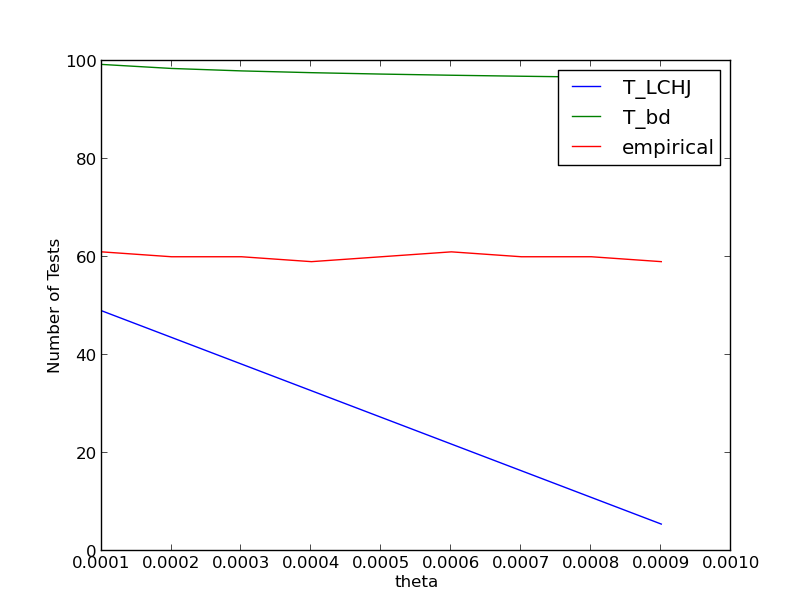
\includegraphics[width=0.5\textwidth]{ubvslb.png}
\caption{Theoretical lower and upper bounds and empirical Test frequencies as functions of \(\theta\)}
\label{ubvslb}
\end{figure}

Note that the Upper bound is not optimal and there still is some room for improvement. Note also that the lower bound degrades with \(\theta_i \). The lower bound (\(T_{LCHJ}\)) was generated according to theorem (\ref{thm:upper}). 

\begin{figure}[h]
\centering
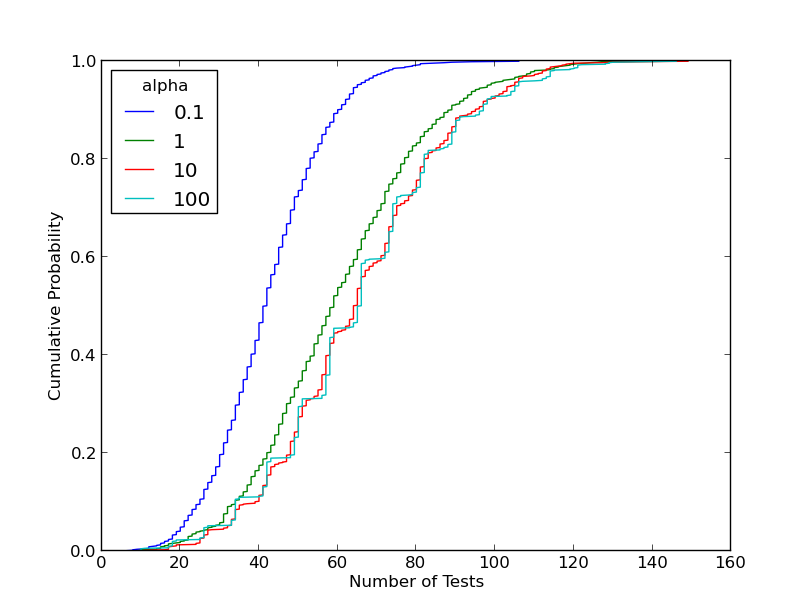
\includegraphics[width=0.5\textwidth]{variousalpha.png}
\caption{Cumulative distribution curves of the modified Hwang algorithm with fixed \(\theta = 0.0001\) and \(\alpha\) varying }
\label{testsvsalpha}
\end{figure}

\begin{figure}[h]
\centering
\includegraphics[width=0.5\textwidth]{nicegraphlaminar.png}
\caption{Cumulative distribution curves for fixed \(\alpha = 1\) and varying \(\theta\)}
\label{testsvstheta}
\end{figure}

Figures (\ref{testsvsalpha}) and (\ref{testsvstheta}) show that the performance is relatively insensitive to the cut-off \(\theta\), and more sensitive to the uniformity (or otherwise) of the probability distribution \(\vc{p}\). Heuristically, this is for because distributions which are highly concentrated on a few items algorithms can make substantial savings on the testing budget by testing those highly likely items first (which is captured in the bin structure of the above algorithm). 

The insensitivity to the cutoff \(\theta\) is due to items below \(\theta\) being overwhelmingly unlikely to be defective - which for small \(\theta\) means that few items (relative to the size of the problem) get discarded.

\section{Discussion}
%
We have introduced and analysed an algorithm for Probabilistic group testing which uses `just over' $H(\vc{U})$ tests to
recover all the defectives with high probability. Combined with a weak converse taken from \cite{li5}, this allows us to deduce that
the weak capacity of Probabilistic group testing is $C=1$.  
These results are illustrated by simulation.

For simplicity, this work has concentrated on establishing a bound $T_{\bd}$ in \eqref{eq:tbd} which has leading term $H(\vc{U})$,
and not on tightening bounds on the coefficient of $\mu$ in \eqref{eq:tbd}. For completeness, we mention that this coefficient
can be reduced from 3, under a simple further condition:

\begin{remark}
For some $c \leq 1/2$, we assume that all the $p_i \leq c$, and we alter the definition of `fullness' to assume that a set is
full if it has total probability less than $\alpha$. In this case, the term $P_{\setS} \log_2 P_{\setS}$ in \eqref{eq:tbds}
becomes $P_{\setS} \log_2 (\alpha + c)$, the bound in \eqref{eq:counting} becomes $\mu/\alpha$, and since
$\left( (1-p) \log_2 (1-p) \right)/p$ is decreasing in $p$, we can add a term $(1-c) \log_2 (1-c) $ to \eqref{eq:toopt}.
Overall, the coefficient of $\mu$ becomes $f(a,c) := \log_2 (\alpha + c) + 1 + 1/\alpha + (1-c) \log_2(1-c)$, which we can optimize over
$\alpha$. For example, if $c = 1/4$, taking $\alpha = 0.88824$, we obtain $f(a,c) = 2.00135$.
\end{remark}

It remains of interest to tighten the upper bound of Theorem \ref{thm:upper},
in order prove a strong converse, and hence confirm that the strong capacity is also equal to $1$.

In future work, we hope to explore more realistic models of defectivity, such as those where the defectivity of $U_i$ are not
necessarily independent, for example by imposing a Markov neighbourhood structure.



%
% And the appendix goes here
%\appendix
%\import{chapters/appendices/}{app0A.tex}
%\clearemptydoublepage
%
% Apparently the guidelines don't say anything about citations or
% bibliography styles so I guess we can use anything.
\backmatter
\printglossary[type=\acronymtype,title=Abbreviations]

%\refstepcounter{chapter}
\bibliography{thesis2}
\clearemptydoublepage
\end{document}